\chapter{Orchestrating Transformation Networks 
    \pgsize{60 p.}
}
\label{chap:orchestration}

\mnote{Application function in transformation networks}
A transformation network is composed of transformations and an application function, which executes the transformations in an order determined by an orchestration function.
In the previous chapters, we have discussed how the individual transformations can be defined and which properties they have to fulfill to be properly usable in a transformation network.
In the following, we discuss how the combination of transformations, as the second essential part of a transformation network, can be realized by an application function.

\mnote{Correctness of application functions}
Although the behavior of an application function has already been defined in \autoref{def:applicationfunction}, we have shortly discussed that we cannot require correctness for such a function in the sense that it always yields consistent models for every given models and changes to them.
We will prove that statement and show that this can either be because there is no execution order of the given transformations that yields consistent models for given models and changes to them or, even if it exists, it may not be possible to find it.

\mnote{Requirements for transformations}
In this chapter, we thus discuss under which conditions we can require an application function to return consistent models.
We derive an algorithm that realizes an application function and prove that it is not possible to ensure its termination without further restrictions to the transformations or the cases in which the algorithm is expected to return consistent models.
The discussion of different restriction options gives us the insight that none of them is practically applicable, because they restrict expressiveness of transformations and transformation networks too much.
Thus, we finally propose an algorithm that operates conservatively, i.e., if it returns models they are consistent, but it may not always return consistent models although an execution order of transformations that yields them exists.
That algorithm is supposed to improve the ability of a transformation developer to identify why no execution order of transformations could be found although it existed.
We have envisioned this as the \emph{comprehensibility} property in \autoref{chap:introduction:consistency:orchestration}.

\mnote{Undecidability of orchestration problem, practical algorithm}
This chapter thus constitutes our contribution \autoref{contrib:correctness:orchestration}, which consists of four subordinate contributions:
a discussion of the design of an application function with possible bounds for the number of executions and a notion of optimality leading to the definition of the \emph{orchestration problem}; the derivation of an algorithm for an application function, for which we discuss termination, prove undecidability of the orchestration problem and discuss different strategies to restrict transformations such that the orchestration problem becomes decidable; a gradual definition of optimality of an application function and a discussion of its systematic improvement; and finally the proposal of an algorithm that operates conservatively based on well-defined properties that ensure its termination and help to find the reasons whenever no execution order of transformations yielding consistent models is found.
It answers the following research question:

\researchquestionrepeat{rq:correctness:orchestration}

\mnote{Benefits: systematic knowledge and concrete algorithm}
While existing approaches to orchestrate transformations are restricted to specific network topologies, our approach is supposed to not restrict the supported topology in any way.
Existing work proposes, for example, to define an execution order explicitly~\cite{pilgrim2008a, vanhooff2007UniTI-MODELS} or to derive a topological order~\cite{stevens2020BidirectionalTransformationLarge-SoSym}, which restricts the topologies to those in which a transformation needs to be executed only once.
We prove that it is not possible to orchestrate arbitrary transformations such that they always yield consistent models whenever that is possible, i.e., when an according execution order of the transformations exists.
We do, however, come up with an algorithm that is able to process transformation networks of arbitrary topology, which follows a specific orchestration strategy that does not necessarily find an execution order that yields consistent models whenever it exists, but instead is defined in way that it supports the transformation developer or user in finding the reason for the inability to find such an order.
On the one hand, this gives transformation developers systematic knowledge about limitations regarding the possibility to orchestrate transformations and, on the other hand, gives them an algorithm for the orchestration to be readily applied.

\mnote{Publication of contributions}
Selected insights presented in this chapter have been developed in a scientific internship together with Joshua Gleitze, which was supervised by the author of this thesis, and have already been published~\cite{gleitze2020orchestration}.

% 1. Application function can return $\bot$ (or not terminate), what are the reasons that it needs to return $\bot$ or does not terminate?
% 1.1. In best case algorithm returns consistent models
% 1.2. If it does not, it may return $\bot$, return inconsistent models (is excluded by construction) or not terminate at all
% 1.3. When should it return $\bot$? Design Space for Functions
% 1.4. Why does it not terminate? Divergence/Alternation
% 2. Restriction to the Application Function
% 2.1. Execution Bound
% 2.2. Show Undecidability -> cannot find an orchestration although it exists
% 3. What restrictions can we make to transformation to, first, ensure that an orchestration exists and, second, it can be found?
% 3.1. Monotony

%\todo{Do we discuss somewhere that orchestration/application should be generic, independent from the concrete network? Maybe define this as the central goal in this section. The general problem in the notion chapter may also allow problem specific realizations. In fact, a parameterized function as in the formalization is specific to the transformations anyway. An algorithm, however, may be generic or specific. So discuss that property in the algorithm section.}

%\todo{Introduce term of \emph{interoperability} of transformations (i.e. that they select the same options and things like that), but rather informally}

\todoLater{Who returns $\bot$ when no order exists? Orc or app?}
%\todo{Define the "orchestration problem"} % and any short form of "orchestration that yields consistent models}

%\todo{Theorem: The shortest consistent orchestration can be arbitrarily long (unbounded executions)}

%\todo{Theorem for single execution: Only orchestrations in O(n) excludes consistent orchestrations}

\section{Orchestration Goals and Problem Statement} % The Orchestration Problem % Design Space for the Orchestration Function} % and orchestration function

\mnote{Undefined when application function is expected to return consistent models}
To recapitulate, the definition of an application function for transformation networks, given in \autoref{def:applicationfunction}, requires an application function $\appfunction{\orcfunction{\transformationset{T}}}$ to accept models and changes to them and yields either a tuple of models or $\bot$.
Whenever it returns a tuple of models, they must be achieved by applying the transformations in $\transformationset{T}$ of the network in an order determined by the orchestration function $\orcfunction{\transformationset{T}}$.
We then say that this execution order is an \emph{orchestration} of the transformations and that the execution of transformations in that order \emph{yields} those models.
The notion of correctness for the application function given in \autoref{def:applicationfunctioncorrectness} additionally requires the returned models to be consistent.
We did, however, not yet define when we expect the function to return consistent models and when we allow it to return $\bot$, as this requires further discussion of the alternatives, which we make in the following.

\mnote{Application function highly depends on orchestration function}
In fact, the application function highly depends on the results of the orchestration function.
If that function does not deliver an orchestration that yields consistent models, a correct application function may only return $\bot$.
Thus, we are specifically concerned with ensuring that the orchestration function finds an orchestration that yields consistent models as often as possible.
We call an orchestration that yields consistent models a \emph{consistent orchestration}.
Precisely, we define an orchestration and a consistent orchestration as follows.

\begin{definition}[Orchestration]
    Let $\transformationset{T}$ be a set of transformation.
    We call any sequence of those transformations $\sequenced{\transformation{t}_{1}, \transformation{t}_{2}, \dots} \in \transformationset{T}^{< \mathbb{N}} \equalsperdefinition \emptyset \cup \transformationset{T}^1 \cup \transformationset{T}^2 \cup \dots$ an \emph{orchestration} of them.

    For models $\modeltuple{m} \in \metamodeltuple{M}$ and changes $\changetuple{\metamodeltuple{M}} \in \changeuniverse{\metamodeltuple{M}}$, we say that an orchestration $\sequenced{\transformation{t}_{1}, \dots, \transformation{t}_{n}}$ is \emph{consistent} if, and only if, the subsequent application of the transformations to $\modeltuple{m}$ and $\changetuple{\metamodeltuple{M}}$  is consistent, i.e., $\generalizationfunction{\metamodeltuple{M},\transformation{t}_{n}} \concatfunction \dots \concatfunction \generalizationfunction{\metamodeltuple{M},\transformation{t}_{1}}(\modeltuple{m}, \changetuple{\metamodeltuple{M}}) \consistenttomath \transformationset{T}$.
\end{definition}

\mnote{Orchestration function is allowed to return arbitrary long sequences of transformations}
The definition of an orchestration function allows it to determine an arbitrary long sequence of transformations, also including each transformation multiple times.
While we introduced this general notion to avoid unnecessary restrictions, in the following we show the necessity of having this general notion, rather than allowing each transformation to be executed only once, as proposed by existing work, such as \cite{stevens2020BidirectionalTransformationLarge-SoSym}.
From the insight that we need to allow transformations to be executed multiple times, we derive and discuss when we expect the application function to return consistent models, to finally come up with a notion of \emph{optimality} for the orchestration function determining the execution order.
This leads to the definition of the central \emph{orchestration problem} that we want a transformation network to solve.

% Discuss options for realizing the functions:
% Orchestration returns only sequence with each transformation executed once vs. arbitrary number of executions

% \begin{itemize}
%     \item We introduced a transformation network as a set of transformations, and an application function that uses an orchestration function to determine the execution order of the transformations for a given input
%     \item An application function may return $\bot$ or consistent models to be correct.
%     \item It may always return $\bot$ to be correct, this is however not what we want.
%     \item It would be intuitive to expect an application function to always return consistent models when there is an execution order of the transformations (i.e. an orchestration) that delivers consistent models.
%     \item So, we first investigate whether we can define a bound for the number of necessary transformation executions.
%     \item We there conclude, that we cannot restrict the number of necessary transformation execution
% \end{itemize}


\subsection{Single Transformation Execution}

\mnote{Ranges for possible numbers of transformation executions}
The possible number of executions for transformations of network range from a selected execution, e.g., in terms of spanning tree, over the execution of each transformation for one or a fixed number of times, to an arbitrary number of executions per transformations.
In the following, we will motivate why the single execution of each transformation is not sufficient in practice and prove that there can be cases in which it is not sufficient.

\mnote{Spanning trees are not sufficient}
The even stronger restriction to spanning trees is obviously not sufficient.
Consider the following consistency relations. For reasons of simplicity, we use \modellevelconsistencyrelations instead of fine-grained relations:
\begin{align*}
    & 
    \consistencyrelation{CR}{12} = \setted{\tupled{\model{m}{1}, \model{m}{2}}, \tupled{\model{m}{1}, \model{m}{2}'}, \tupled{\model{m}{1}', \model{m}{2}'}, \tupled{\model{m}{1}', \model{m}{2}''}} \\
    & 
    \consistencyrelation{CR}{13} = \setted{\tupled{\model{m}{1}, \model{m}{3}}, \tupled{\model{m}{1}, \model{m}{3}''}, \tupled{\model{m}{1}', \model{m}{3}}, \tupled{\model{m}{1}', \model{m}{3}'}} \\
    & 
    \consistencyrelation{CR}{23} = \setted{\tupled{\model{m}{2}, \model{m}{3}}, \tupled{\model{m}{2}', \model{m}{3}'}, \tupled{\model{m}{2}', \model{m}{3}''}, \tupled{\model{m}{2}'', \model{m}{3}}} 
\end{align*}
%We consider the set of these relations with their transposed ones: $\consistencyrelationset{CR} = \setted{\consistencyrelation{CR}{12}, \consistencyrelation{CR}{12}^T, \consistencyrelation{CR}{13}, \consistencyrelation{CR}{13}^T, \consistencyrelation{CR}{23}, \consistencyrelation{CR}{23}^T}$.
That set of relations is compatible according to \autoref{def:compatibility}, because for each model there is a containing tuple of models that is consistent.
For the initial tuple of models $\tupled{\model{m}{1}, \model{m}{2}, \model{m}{3}}$, we consider a change that changes $\model{m}{1}$ to $\model{m}{1}'$.
Then we can distinguish tree possibly spanning trees of transformations that try to restore consistency, which we denote with $\transformation{t}_{12}, \transformation{t}_{13}, \transformation{t}_{23}$ for the according consistency relations.
Each tree consists of two transformations.
\begin{properdescription}
    \item[$\transformation{t}_{12}$, $\transformation{t}_{13}$:] 
    $\transformation{t}_{12}$ may change $\model{m}{2}$ to $\model{m}{2}'$. $\transformation{t}_{13}$ does nothing, because $\model{m}{1}'$ and $\model{m}{3}$ are already consistent to $\consistencyrelation{CR}{13}$.
    $\model{m}{2}'$ and $\model{m}{3}$ are, however, not consistent to $\consistencyrelation{CR}{23}$.
    \item[$\transformation{t}_{12}$, $\transformation{t}_{23}$:] 
    Like before, $\transformation{t}_{12}$ may change $\model{m}{2}$ to $\model{m}{2}'$. 
    $\transformation{t}_{23}$ may then change $\model{m}{3}$ to $\model{m}{3}''$. 
    $\model{m}{1}'$ and $\model{m}{3}''$ are, however, not consistent to $\consistencyrelation{CR}{13}$.
    \item[$\transformation{t}_{13}$, $\transformation{t}_{23}$:]
    $\transformation{t}_{13}$ may do nothing, because $\model{m}{1}'$ and $\model{m}{3}$ are already consistent to $\consistencyrelation{CR}{13}$.
    $\transformation{t}_{23}$ does also nothing, because $\model{m}{2}$ and $\model{m}{3}$ are still consistent to $\consistencyrelation{CR}{23}$.
    $\model{m}{1}'$ and $\model{m}{2}$ are, however, not consistent to $\consistencyrelation{CR}{12}$.
\end{properdescription}

\mnote{Each transformation needs to be executed at least once}
Thus, we need to execute each transformation at least once, because each transformation is only responsible for restoring its consistency relations and thus we cannot expect the resulting models to be consistent if some transformation were not executed, although the involved models were changed by other transformations.
However, restricting the execution to each transformation once is not appropriate either.
To show that, we consider examples that we derived from those we have already presented in \owncite{gleitze2020orchestration}, which used a different scenario context.

\begin{figure}
    \centering
    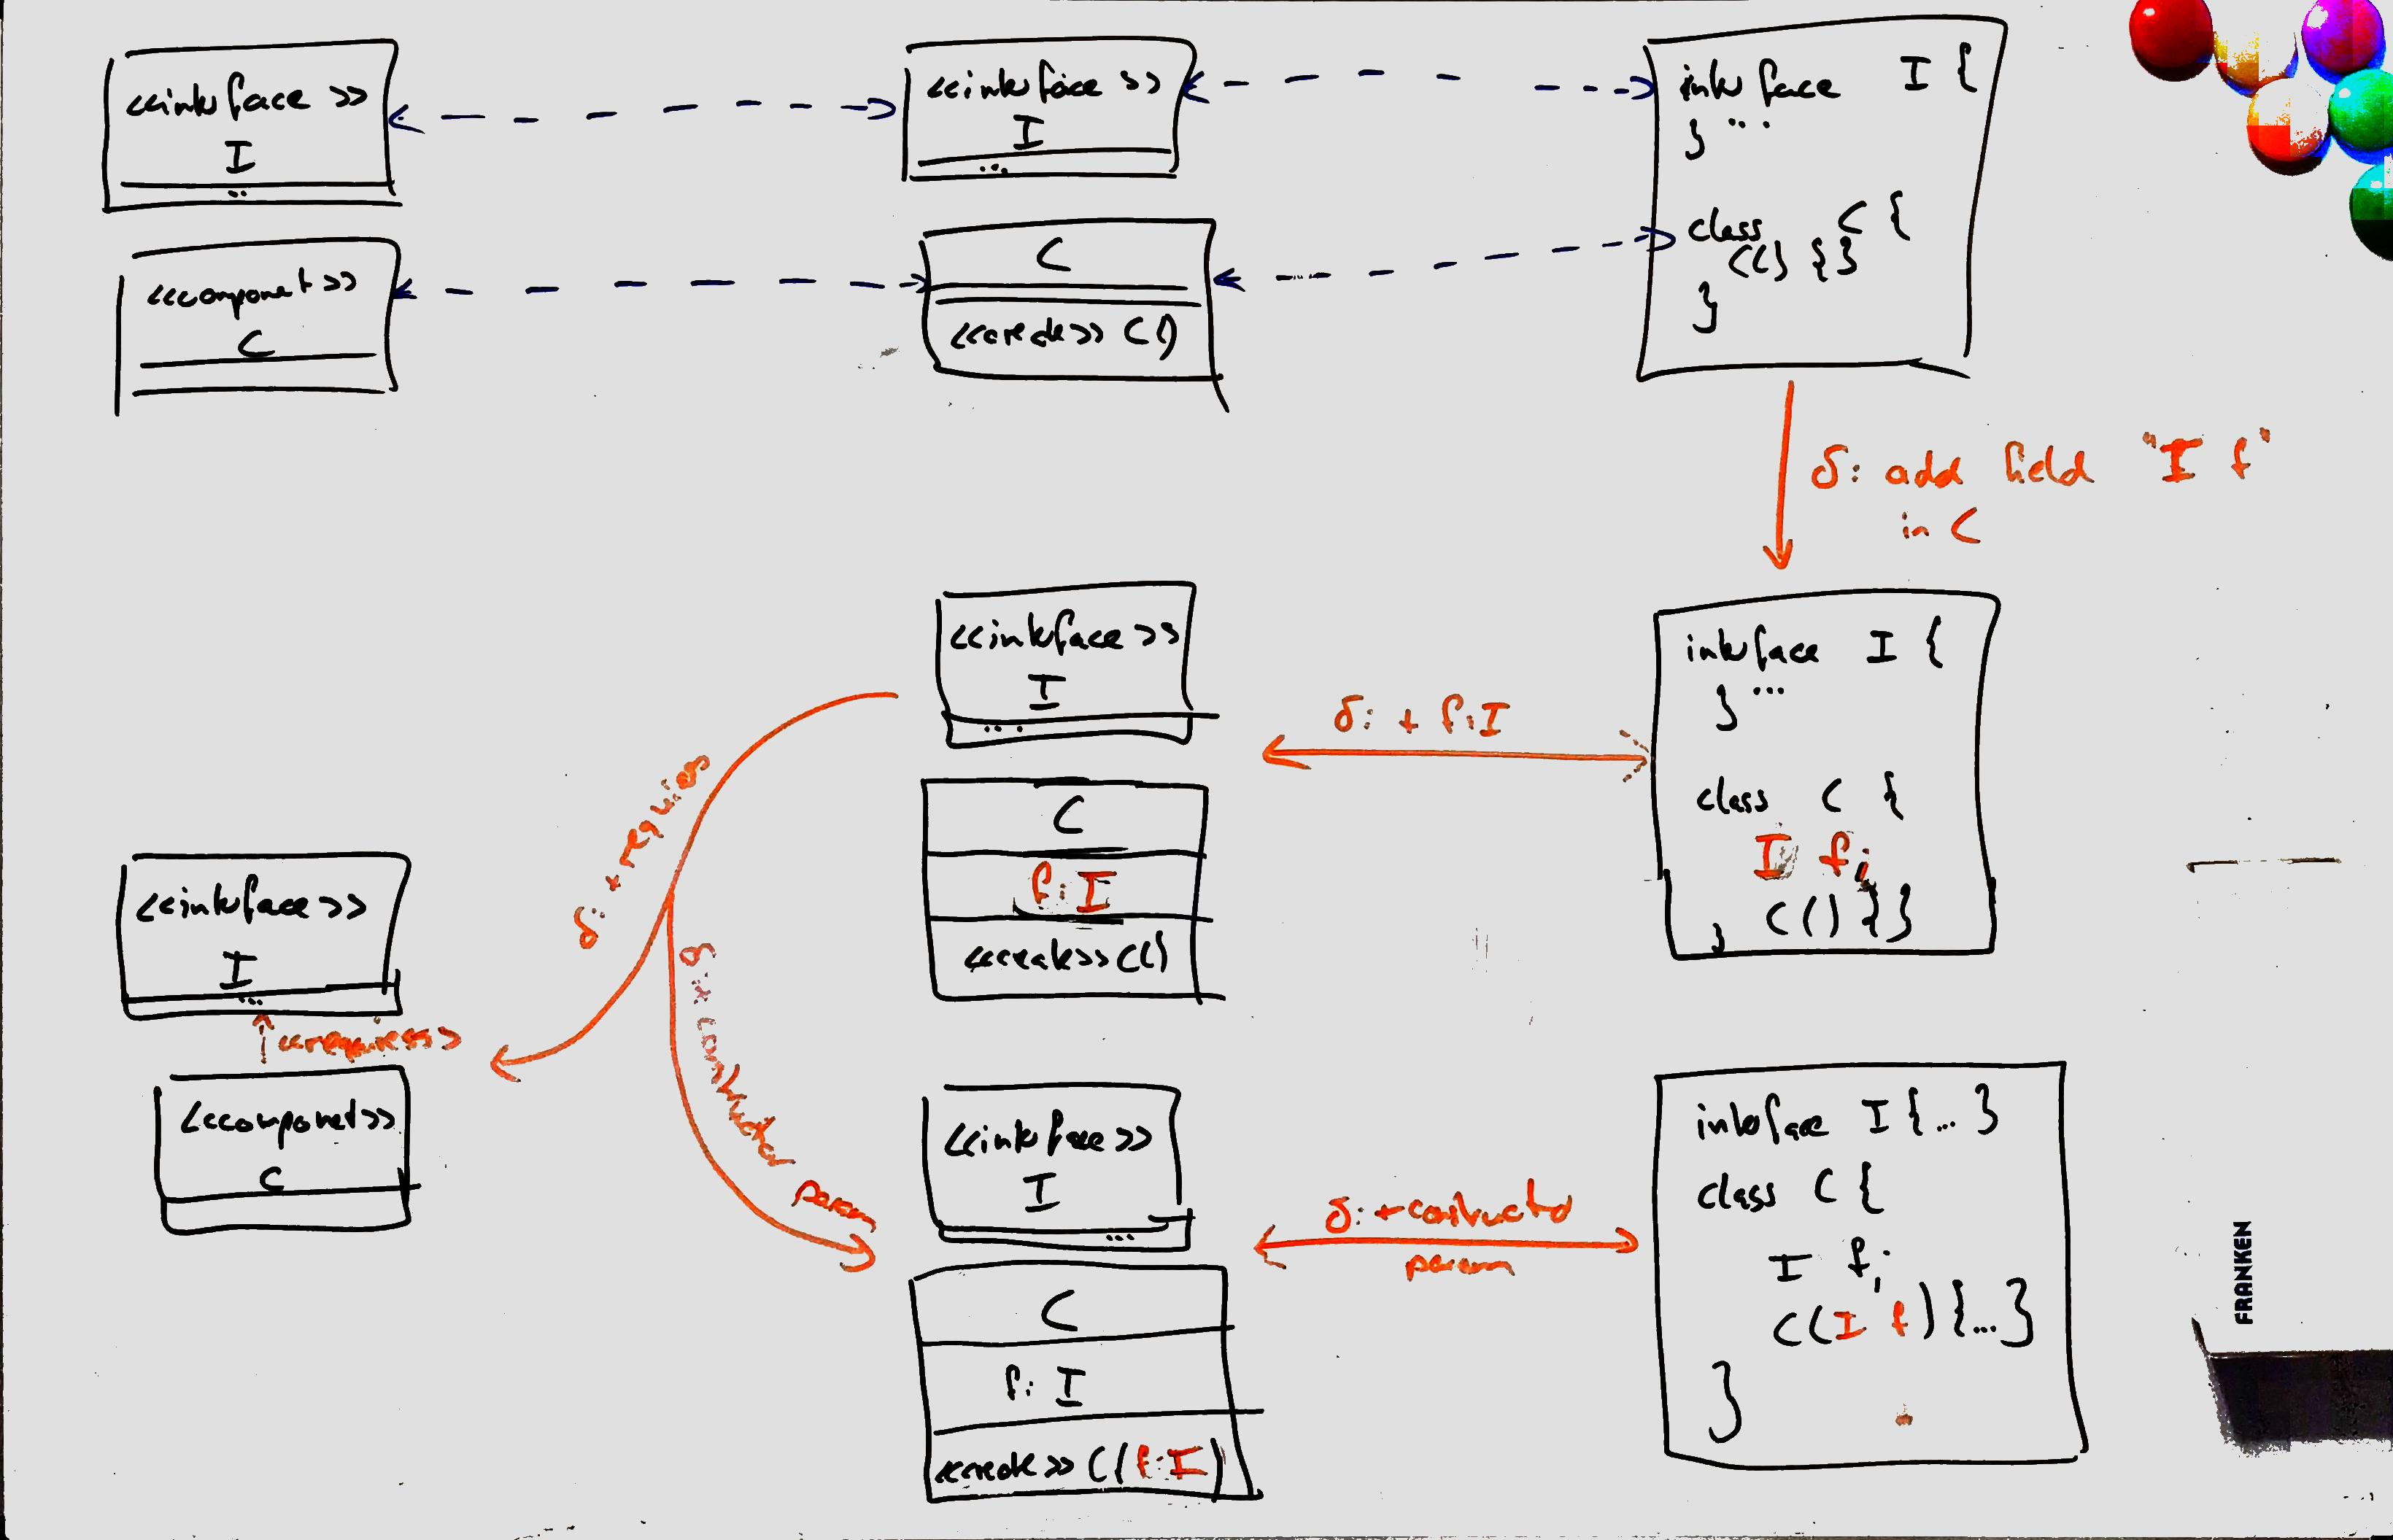
\includegraphics[width=\textwidth]{figures/correctness/orchestration/necessity_multiple_executions.jpg}
    \caption[Necessity of executing a transformation multiple times]{Necessity of executing a transformation multiple times.}
    \label{fig:orchestration:necessity_multiple_executions}
\end{figure}

\mnote{Example for component requires relation between \gls{PCM}, UML and Java}
Consider the example in \autoref{fig:orchestration:necessity_multiple_executions}, which describes the example depicted in \autoref{fig:introduction:scenario_duplicate_execution} within the introduction more precisely.
In the example, interfaces in UML and Java are related to architectural interfaces in a \gls{PCM} model.
\gls{PCM} components are realized by equally named classes in UML and Java.
Additionally, when a \gls{PCM} component requires an interface, this is realized by a field with the interface type in the component-realization class in UML and Java and an appropriate constructor argument.
Consistency is defined by transformations between \gls{PCM} and UML, as well as between UML and Java.

\mnote{Scenario requiring duplicate execution of one transformation}
In the scenario in \autoref{fig:orchestration:necessity_multiple_executions}, we begin with a consistent state of one interface and component, each realized by an interface and class, respectively, in both UML and Java.
A user then introduces a change of the Java code, in which he adds a field of the interface type to the component-realization class in Java.
The transformation between UML and Java propagates this change to the UML model, such that both models are consistent again.
The transformation between \gls{PCM} and UML then detects that the added field is of the type of an architectural interface, thus representing a requires relation between the corresponding component and the architectural interface. 
It adds the appropriate requires relation in the \gls{PCM} model, but also adds an appropriate parameter to the constructor of the component-realization class in UML, as required by the consistency relations.
This introduces a further inconsistency between the UML and the Java model, which requires the transformation between UML and Java to be executed again to also add that constructor parameter in the Java code.

\mnote{Cycles in transformation networks do not reduce necessary number of executions}
We simplified the example to the necessary core, although in practice a further transformation between \gls{PCM} and Java would be required, for example, to ensure that the field is set within the constructor.
One might argue that having a cycle of transformations between \gls{PCM}, UML and Java could resolve the problem, as the necessary second execution of the transformation between UML and Java is not necessary if the information is propagated from \gls{PCM} to Java.
This is, however, only true if exactly that order of transformations is chosen for execution and if the transformation between \gls{PCM} and Java does not introduce further information in the Java model that then needs to be propagated to UML.

\mnote{Synchronizing transformations can change models already processed by other transformation}
In general, it is always possible that transformations need to react to the changes performed by other, if they are not in some way aligned to each other.
This is due to the fact that a synchronizing transformation may change both models, thus if one transformation restores consistency between two models and another transformation reacts to that by restoring consistency between one of these models and another one, then both these models become changes, thus requiring the first transformation to process the newly created changes again.

\begin{figure}
    \centering
    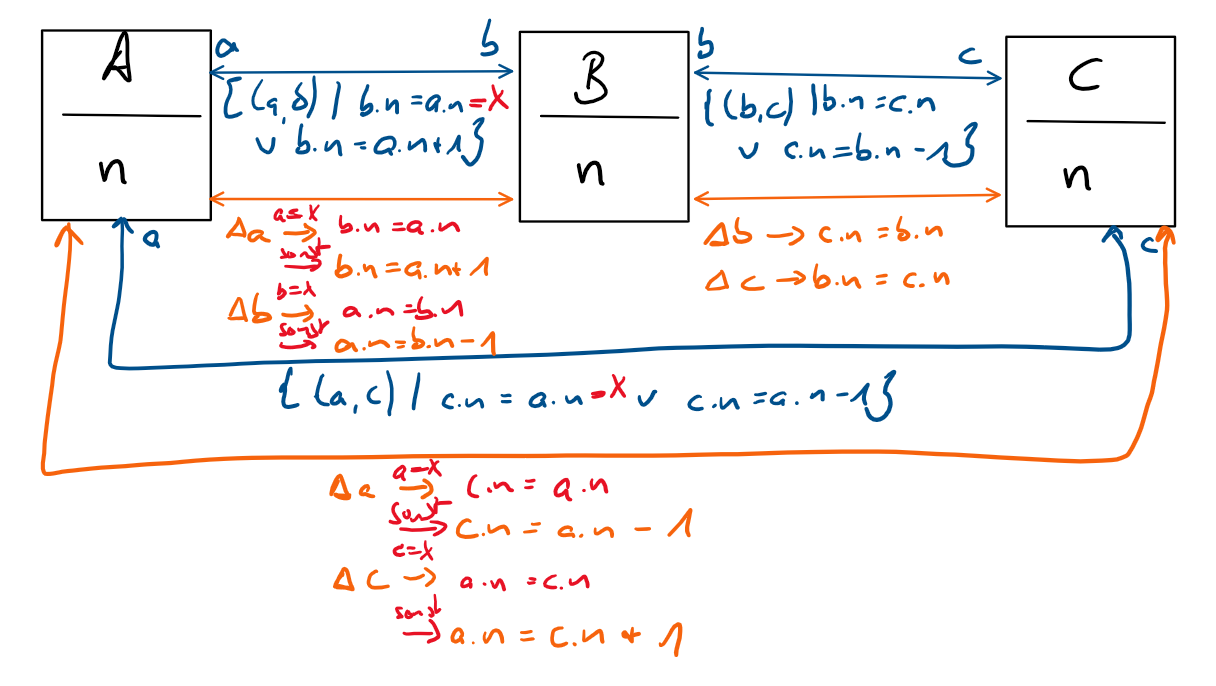
\includegraphics[width=\textwidth]{figures/correctness/orchestration/no_upper_bound_example.png}
    \caption[Example for arbitrary bounds of transformation execution]{Example for an arbitrary bound of necessary transformation execution depending on value of $x$.}
    \todo{Ist das b.n-1 zwischen B und C in der Relation richtig? Das muss doch weg?}
    \label{fig:orchestration:no_upper_bound}
\end{figure}

\mnote{Generalization to a theoretical incrementation example}
We can generalize the previous example to the one given in \autoref{fig:orchestration:no_upper_bound}.
It is an extension of the example given in \autoref{fig:synchronization:multiple_unidirectional_execution} for the necessity to execute the consistency preservation rules of a bidirectional transformation multiple times.
This also applies to the case in which multiple bidirectional transformations are combined.
The depicted relations and the informally defined consistency preservation rules require that elements \modelelement{A}, \modelelement{B} and \modelelement{C} with the same value of $n$ exist, and that for each \modelelement{A} with value $n$ a \modelelement{B} and \modelelement{C} with $n$ incremented by $1$ exist, except for the case that $n = x-1$.
In consequence, for an \modelelement{A} with $n = i$, all \modelelement{A}, \modelelement{B} and \modelelement{C} with $i \leq n < x$ need to exist.
This, obviously, requires the transformations to be executed $x-1-i$ times.

\mnote{Precise definition of transformation network}
We prove the informally given statement with the following precise definition of the transformations for a variable value of $x$.
Let $\class{A}{}, \class{B}{}, \class{C}{}$ be the classes depicted in \autoref{fig:orchestration:necessity_multiple_executions}.
\begin{align*}
    & 
    \metamodelinstanceset{M}{1} = \mathcal{P}(\instances{\class{A}{}}), %\\
    %& 
    \metamodelinstanceset{M}{2} = \mathcal{P}(\instances{\class{B}{}}), %\\
    %& 
    \metamodelinstanceset{M}{3} = \mathcal{P}(\instances{\class{C}{}}) \\[1em]
    &
    \consistencyrelation{CR}{12} = \setted{\tupled{a,b} \in \instances{\class{A}{}} \times \instances{\class{B}{}} \mid b.n = a.n + 1 \neq x}, \consistencyrelationset{CR}_{12} = \setted{\consistencyrelation{CR}{12}, \consistencyrelation{CR}{12}^T} \\
    &
    \consistencypreservationrule{\consistencyrelationset{CR}_{12}}^{\rightarrow}(\model{m}{1}, \model{m}{2}, \change{\metamodel{M}{1}}) = \change{\metamodel{M}{2}} \\
    & \formulaskip
    \withmath \change{\metamodel{M}{2}}(\model{m}{2}) = \setted{b \in \instances{\class{B}{}} \mid \exists a \in \change{\metamodel{M}{1}}(\model{m}{1}) : b.n = a.n + 1 \neq x} \\
    & 
    \consistencypreservationrule{\consistencyrelationset{CR}_{12}}^{\leftarrow}(\model{m}{2}, \model{m}{1}, \change{\metamodel{M}{2}}) = \change{\metamodel{M}{1}} \\
    & \formulaskip
    \withmath \change{\metamodel{M}{1}}(\model{m}{1}) = \setted{a \in \instances{\class{A}{}} \mid \exists b \in \change{\metamodel{M}{2}}(\model{m}{2}) : b.n = a.n + 1 \neq x \land a \geq 0} \\
    &
    \transformation{t}_{12} = \tupled{\consistencyrelationset{CR}_{12}, \consistencypreservationrule{\consistencyrelationset{CR}_{12}}^{\rightarrow}, \consistencypreservationrule{\consistencyrelationset{CR}_{12}}^{\leftarrow}} \\[1em]
    & 
    \consistencyrelation{CR}{13} = \setted{\tupled{a,c} \in \instances{\class{A}{}} \times \instances{\class{C}{}} \mid c.n = a.n}, \consistencyrelationset{CR}_{13} = \setted{\consistencyrelation{CR}{13}, \consistencyrelation{CR}{13}^T} \\
    & 
    \consistencypreservationrule{\consistencyrelationset{CR}_{13}}^{\rightarrow}(\model{m}{1}, \model{m}{3}, \change{\metamodel{M}{1}}) = \change{\metamodel{M}{3}} \\
    & \formulaskip
    \withmath \change{\metamodel{M}{3}}(\model{m}{3}) = \setted{c \in \instances{\class{C}{}} \mid \exists a \in \change{\metamodel{M}{1}}(\model{m}{1}) : c.n = a.n} \\
    & 
    \consistencypreservationrule{\consistencyrelationset{CR}_{13}}^{\leftarrow}(\model{m}{3}, \model{m}{1}, \change{\metamodel{M}{3}}) = \change{\metamodel{M}{1}} \\
    & \formulaskip
    \withmath \change{\metamodel{M}{1}}(\model{m}{1}) = \setted{a \in \instances{\class{A}{}} \mid \exists c \in \change{\metamodel{M}{3}}(\model{m}{3}) : c.n = a.n} \\
    & 
    \transformation{t}_{13} = \tupled{\consistencyrelationset{CR}_{13}, \consistencypreservationrule{\consistencyrelationset{CR}_{13}}^{\rightarrow}, \consistencypreservationrule{\consistencyrelationset{CR}_{13}}^{\leftarrow}} \\[1em]
    &
    \consistencyrelation{CR}{23} = \setted{\tupled{b,c} \in \instances{\class{B}{}} \times \instances{\class{C}{}} \mid c.n = b.n}, \consistencyrelationset{CR}_{23} = \setted{\consistencyrelation{CR}{23}, \consistencyrelation{CR}{23}^T} \\
    & 
    \consistencypreservationrule{\consistencyrelationset{CR}_{23}}^{\rightarrow}, \consistencypreservationrule{\consistencyrelationset{CR}_{23}}^{\leftarrow} \andmath \transformation{t}_{23} \mathtextspacearound{accordingly} \\[1em]
    &
    \consistencyrelationset{CR} = \consistencyrelationset{CR}_{12} \cup \consistencyrelationset{CR}_{13} \cup \consistencyrelationset{CR}_{23} \\
    &
    \transformationset{T}_{inc} = \setted{\transformation{t}_{12}, \transformation{t}_{13}, \transformation{t}_{23}}
\end{align*}

\mnote{Proof that single execution of each transformation is not sufficient in scenario}
For these transformations, we are able to show that the transformation $\transformation{t}_{12}$ needs to be executed a minimal number of depending on $x$ for a specific input.
Thus, it is not sufficient to execute each transformation only once in this network.

\begin{lemma}[Minimal Number of Transformation Executions]
    \label{lemma:minimal_executions}
    Let $\transformationset{T}_{inc}$ be the previously defined set of transformations and let $\model{m}{1} = \model{m}{2} = \model{m}{3} = \emptyset$ be empty models and $\change{\metamodel{M}{1}} \in \changeuniverse{\metamodel{M}{1}}$ a change with $\change{\metamodel{M}{1}}(\model{m}{1}) = \setted{a \in \instances{\class{A}{}} \mid a.n = 0}$.
    Then the result of every orchestration function $\orcfunction{\transformationset{T}_{inc}}$ with $\appfunction{\orcfunction{\transformationset{T}_{inc}}}(\tupled{\model{m}{1},\model{m}{2},\model{m}{3}},\tupled{\change{\metamodel{M}{1}},\identitychange,\identitychange}) \consistenttomath \consistencyrelationset{CR}$ contains $\transformation{t}_{12}$ at least $x-1$ times.
\end{lemma}
\begin{proof}
    $\appfunction{\orcfunction{\transformationset{T}_{inc}}}$ can only return consistent models when it applies the transformations in the order delivered by $\orcfunction{\transformationset{T}_{inc}}$ by definition in \autoref{def:applicationfunction}.
    We thus consider any order of transformations, as delivered by any orchestration function, to show that it contains $\transformation{t}_{12}$ at least $x-1$ times to deliver consistent models.
    
    Let $max_n(\model{m}{1},\model{m}{2},\model{m}{3}) = max\setted{e.n \mid e \in \model{m}{1} \cup \model{m}{2} \cup \model{m}{3}}$ be the maximal value of $n$ in any instance of \modelelement{A}, \modelelement{B} and \modelelement{C} in any given models $\model{m}{1}$, $\model{m}{2}$ and $\model{m}{3}$. In the following, we shortly note $max_n$ if the concrete models are currently not relevant.

    \begin{properdescription}
        \item[Executing $\transformation{t}_{13}$ and $\transformation{t}_{23}$ an arbitrary number of times does not increase $max_n$:]
        The transformations do only ensure that for any given models the returned models contain all elements with the same values of $n$ and do not introduce new elements with values of $n$ larger than the existing ones.
        \item[A single execution of $\transformation{t}_{12}$ increases $max_n$ by at most one:]
        There is no \modelelement{A} or \modelelement{B} with $n > max_n$.
        For every \modelelement{A} with $n < max_n$, $\transformation{t}_{12}$ creates, if necessary, a \modelelement{B} with value $n + 1 \leq max_n$, thus not increasing $max_n$.
        For every \modelelement{B} with $n \leq max_n$, it creates, if necessary, an \modelelement{A} with value $n-1 < max_n$.
        For every \modelelement{A} with $n = max_n$, a \modelelement{B} with value $n+1 = max_n + 1$ is creates, as long as $n \neq x-1$.
        For the newly created \modelelement{B}, no further elements needs to be created to fulfill the consistency relations.
        Thus, $max_n$ is, at most, increased by $1$.
        \item[ When $max_n(\model{m}{1},\model{m}{2},\model{m}{3}) < x-1$, then $\model{m}{1},\model{m}{2},\model{m}{3}$ are not consistent to $\consistencyrelationset{CR}$:]
        There is at least one element within the models with $n = max_n$.
        If the element with $n = max_n$ is an \modelelement{A}, then there must be a \modelelement{B} with value $n+1$, because of $\consistencyrelationset{CR}_{12}$ and because $n < x-1$.
        But since $n = max_n$, such a \modelelement{B} cannot exist, because otherwise $max_n = n+1$, so this is a contradiction.    
        If the element with $n = max_n$ is a \modelelement{C}, then $\consistencyrelationset{CR}_{13}$ requires an \modelelement{A} with the same value of $n$ to exist and the same argument as before leads to a contradiction.
        Finally, if the element with $n = max_n$ is a \modelelement{B}, then because of $\consistencyrelationset{CR}_{23}$ a \modelelement{C} with the same value must exist and then the same argument as before leads to a contradiction.
    \end{properdescription}

    In summary, we have shown that models $\model{m}{1},\model{m}{2},\model{m}{3}$ are only consistent to $\consistencyrelationset{CR}$ when $max_n(\model{m}{1},\model{m}{2},\model{m}{3}) \geq x-1$.
    Additionally, only $\transformation{t}_{12}$ increases $max_n$ and with each execution it only increases it by at most $1$.
    In consequence, starting with $max_n = 0$, we need at least $x-1$ executions of $\transformation{t}_{12}$ in an arbitrary sequence of the transformations in $\transformationset{T}_{inc}$ to achieve consistent models.
\end{proof}

\mnote{Example transformations can force network to perform an arbitrary number of executions}
We have proven that arbitrary transformation networks can require an arbitrary high number of executions of each transformations.
By selecting an appropriate $x$ in the used example network, we can force the network to perform at least $x$ executions of one transformation to yield a consistent tuple of models.
With this insight, it directly follows that we cannot find an approach to define orchestration functions that delivers sequences containing each transformation only once if we want to ensure that if a consistent orchestration of transformations exists, the approach is supposed to deliver it.

\begin{theorem}[Orchestration with Single Execution]
    \label{theorem:orchestration_single}
    For any set of transformations $\transformationset{T}$, there can be models $\modeltuple{m}$ and changes $\changetuple{}$ to them for which each possible orchestration function $\orcfunction{\transformationset{T}}$ with whom $\appfunction{\orcfunction{\transformationset{T}}}(\modeltuple{m}, \changetuple{})$ is consistent, delivers a sequence as $\orcfunction{\transformationset{T}}(\modeltuple{m}, \changetuple{})$ that contains at least one transformation twice.
\end{theorem}
\begin{proof}
    We know from \autoref{lemma:minimal_executions} that $\transformationset{T}_{inc}$ requires at least $2$ executions of $\transformation{t}_{12}$ for the inputs defined in \autoref{lemma:minimal_executions} when selecting $x \geq 3$.
    This proves the theorem by example.
\end{proof}

\mnote{Example generalizes practical scenario, thus single execution not supposed to be sufficient}
We know from \autoref{theorem:orchestration_single} that if we execute each transformation only once, we may exclude cases for which multiple executions of transformations would have led to a consistent tuple of models.
The example we have given in \autoref{fig:orchestration:necessity_multiple_executions} is a simplification of a realistic transformation scenario, which we generalized to the previous network with transformations $\transformationset{T}_{inc}$.
Thus, we can conclude that the insight is potentially relevant for realistic scenarios.
We should not restrict orchestration to execute each transformation only once, as there can be realistic scenarios in which multiple executions are necessary to find consistent models.
In the following, we thus, for first, allow an arbitrary number of executions of each transformation.

% Essential problem: One transformation may restore consistency between A and B and another between A and C. If then a transformation restores consistency between B and C, the resulting B' and C' may not be consistent A anymore.

% \todo{Beispiel warum mehrfache Ausführung nötig, warum also manche Infos erst durch andere bx reinkommen, die bei einer bx isoliert nicht relevant sind.}

% Bestehende Arbeiten (\cite{stevens2020BidirectionalTransformationLarge-SoSym}) schlagen auch vor eine Baumstruktur zu berechnen (Spannbaum), in dem nur entlang der Baumkanten die Transformationen ausgeführt werden. Dies ist jedoch eine starke Einschränkung daran, was die Transformationen ausdrücken können. Betrachtet man beispielsweise PCM, UML und Java, und hat eine Änderung in PCM. Dann könnte der Spannbaum entweder PCM -> UML -> Java sein, oder PCM -> UML + PCM -> Java. In ersterem Fall würde Verhaltensbeschreibung, die von PCM nach Java übertragen, aber in UML nicht dargestellt wird, nicht übertragen. Im zweiten Fall würde zusätzliche Information zwischen UML und Java nicht propagiert (Beispiel?) --> Hier sollte auf das Properties-Kapitel verwiesen werden, wo diese "Bottlenecks" erklärt sein sollten, inklusive einem Beispiel, die allgemein Baumstrukturen für Transformationsnetwerke ausschließen.

% Consequence: We cannot easily restrict the number of allowed executions. We can define networks that require an arbitrary number of executions.
% Also refer to the synchronization example, where we discussed that.
% Let us, for first, assume that transformations need an arbitrary number of executions.


\subsection{Orchestration Function Behavior} %The Orchestration Problem %Expected Behavior} % Failure Cases} %When to Return $\bot$?}
\label{chap:orchestration:problem:function_behavior}

\mnote{Necessity to define when application function returns $\bot$}
The application function is defined to return models only when they can be derived by applying transformations in an order delivered by the orchestration function and otherwise to return $\bot$.
In addition, we expect a \emph{correct} application function only to deliver models that are consistent.
We did, however, not yet define under which conditions we expect the function not to return $\bot$, because there are different reasons why the function may not be able to deliver consistent models although we could expect it to do so.
In fact, with the current definition, the function is even considered correct if it always returns $\bot$, which is not practical.
Thus, we need to define when exactly we expect the function to return $\bot$.

\mnote{Reasons for not finding an orchestration that yields consistent models}
It might be intuitive to expect an application function to always return consistent models when the input models are consistent and when there is an execution order of the transformations, i.e., an orchestration, that delivers consistent models.
This, in consequence, would lead to the requirement that the orchestration function delivers a sequence of transformations whose application delivers consistent models whenever such a sequence exists for the given models and changes to them.
There can be different reasons why the orchestration function may not deliver such a sequence:
%When is it allowed or needed to return $\bot$?
%It may always return $\bot$ to be correct, this is however not what we want.
%We can distinguish three levels of reasons why the function may not be able to find consistent models:
\begin{properdescription}
    \item[Relations are incompatible:] If the consistency relations are incompatible, a user change may introduce an element for which no consistent models exist. In consequence, the transformation cannot be executed in an order such that the resulting models are consistent and still reflect the given user change.
    %(example with employee for which no consistent other models can be found)
    \item[No orchestration exists:] Even if the relations are compatible, transformations may be defined in a way that they make contradictory decisions for locally consistent solutions. Thus, for a given a change the consistency relations allow different ways to store consistency, of which the transformations always select a way that is not consistent to one of the other relations.
    Then no order of the transformations can restore consistency, although models exist that fulfill consistency for the given change.
    % (example with three options for name mapping with one overlapping, where each transformation always selects the one that is not appropriate for the other). We can further distinguish here whether there is always a change that cannot be processed by a CPR (then the change conflicts with the consistency relations and thus has to be rejected like any change may need to be rejected), or whether an arbitrary long sequence of transformations exists that can be applied but does never yield a consistent set of models.
    \item[No orchestration found:] Finally, although an order of transformations for given changes exists that delivers consistent models, the orchestration function may not deliver it. 
    %finally, the application/orchestration may not be able to find an order of transformations that leads to a consistent state although it exists.
\end{properdescription}

\mnote{Reasons form an induction hierarchy}
These reasons can be considered at different levels, because each of them induces the next, i.e., if there is no orchestration, it cannot be found, and having contradictory relations, there exists no orchestration for some of the changes.
In the end, all of them lead to the situation that no orchestration can be found and, thus, the orchestration function is not able to deliver it.

\mnote{Compatibility can be assumed, existence of an orchestration cannot}
The initially given intuitive requirement that the orchestration function delivers a consistent orchestration whenever it exists would thus assume that the first two levels do not occur and then require the orchestration function to ensure the third.
While we can assume compatibility of the relations, as we discussed how to analyze it in \autoref{chap:compatibility}, we cannot assume that an orchestration does always exists, as we will see in the following.

\mnote{Compatibility does not ensure existence of orchestration}
Although compatibility reduces the chance that an orchestration function does not deliver a consistent orchestration, as we have motivated with the scenario depicted in \autoref{fig:compatibility:unwanted_behavior}, it does not ensure that there is always such a sequence of transformations that the orchestration function can find.
In general, this is always the case when consistency relations define different options for consistency, i.e., they allow the existence of different corresponding elements to consider the models consistent.
Compatibility ensures that there is an overlap of these corresponding elements, such that for every element, for which consistency is restricted, consistent models can be found.
If, however, the consistency preservation rules of the transformations always restore consistency by introducing corresponding elements that are not in this overlap, each transformation will restore consistency locally to its consistency relation, but they can, together, never restore consistency to all consistency relations.

\mnote{Consistency preservation rules need to select overlapping options in consistency relations}
Consider the situation that we have three metamodels $\metamodel{A}{}$, $\metamodel{B}{}$ and $\metamodel{C}{}$ with instances $\model{a}{i}$, $\model{b}{i}$ and $\model{c}{i}$.
Let us assume that those models are uniquely indexed by $i$ and we defined the following consistency relations:
\begin{align*}
    &
    \consistencyrelation{CR}{AB} = \setted{\tupled{\model{a}{i}, \model{b}{k}} \mid k = i} \\
    &
    \consistencyrelation{CR}{AC} = \setted{\tupled{\model{a}{i}, \model{c}{l}} \mid l = i \lor l = i+1} \\
    &
    \consistencyrelation{CR}{BC} = \setted{\tupled{\model{b}{k}, \model{c}{l}} \mid l = k+1 \lor l = k+2}
\end{align*}
This induces the set of consistent model tuples $\setted{\tupled{\model{a}{i}, \model{b}{k}, \model{c}{l}} \mid  i = k = l-1}$, which is given to all three consistency relations.
Thus for any given model we are able to find instances of the other metamodels that are consistent to all consistency relations.
If we define consistency preservation rules for these consistency relations, the ones for $\consistencyrelation{CR}{AC}$ and $\consistencyrelation{CR}{BC}$ may decide between two models to restore consistency.
If $\consistencyrelation{CR}{AC}$ does always select $\model{c}{i}$ for $\model{a}{i}$ and vice versa, and if $\consistencyrelation{CR}{BC}$ does always select $\model{c}{i+2}$ for $\model{a}{i}$ and vice versa, no orchestration of the transformations will yield consistent models, because they never select those models that are in the overlap of the consistency relations.

\begin{figure}
    \centering
    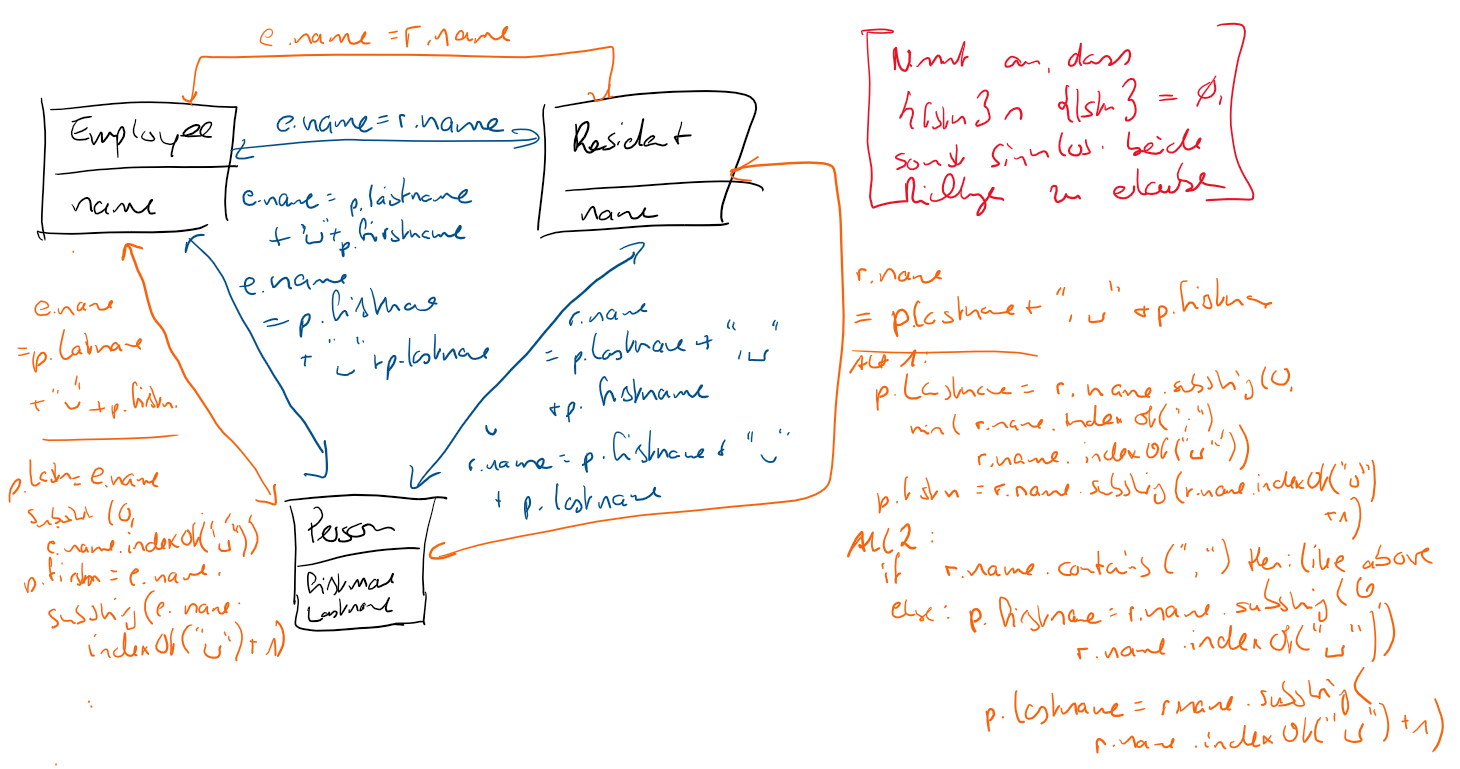
\includegraphics[width=\textwidth]{figures/correctness/orchestration/no_orchestration.png}
    \caption[Consistency preservation rules without orchestration]{Consistency relations with options for corresponding elements leading to consistency preservation rules for which no consistent orchestration exists.}
    \label{fig:orchestration:no_orchestration}
\end{figure}

\mnote{Running example with consistency relations for name composition}
We have already given an abstract example for that problem in \autoref{fig:correctness:no_execution_order}. \autoref{fig:orchestration:no_orchestration}, in addition, demonstrates this situation at a derivation of the running example.
The consistency relation between employees and residents ensures that for each resident and employee there is corresponding other element with the same name.
The consistency relations between employees and persons and between residents and persons ensure that for each person there is a corresponding employee and resident, respectively, but they allow different relations of their names.
While both consider elements corresponding if the name of an employee and resident, respectively, are the concatenation of the first and last name of a person, an employee is also allowed to have the inverse concatenation of last and first name, whereas a resident is also allowed to have this inverse concatenation, but with an additional separation of the last and first name with a comma.
These options for the consistency relations provide further degrees of freedom for each transformation on its own, as they allow, for example, employee names to be encoded differently.
This can, for example, be reasonable if the order of first and last name is not relevant in a model managing employees.
In combination with the other consistency relations, however, the only employees, residents and persons that are considered consistent to all of the consistency relations are those having the same names with the concatenation of first and last name.
Nevertheless, these consistency relations are compatible, because for each possible condition element, i.e., for every possible employee, person and resident, there are consistent models that contain them.

\mnote{Relations in the running example without consistent orchestration}
Consistency relations that preserve these consistency relations need to to choose one of the given options for the names of corresponding employees, residents and persons.
\autoref{fig:orchestration:no_orchestration} sketches consistency preservation rules that make such a selection.
The rules with alternative 1 ensure that for each employee, resident and persons corresponding elements exist, which fulfill those relations of the names that are conflicting.
This means, the employee name is the concatenation of the last and first name of a person, whereas the resident name contains an additional comma in that concatenation.
In the other direction, the names of employees and residents are split at the appropriate indices, given by the whitespace and comma, respectively, to calculate the required first and last name of a person.
In consequence, there is no execution sequence of the transformations that results in consistent models, because the execution of the transformation between employees and persons always leads to a violation of the consistency relation between residents and persons and vice versa.
This is because the transformation between person and resident always introduces a comma in the resident name, which is then appended to the last name by the transformation between employee and persons.
A repeated execution of the transformation repeatedly appends that comma.
On the other hand, the execution of any of the transformation does never lead to the introduction of a person that fulfills the non-conflicting conditions of both consistency relations by simply containing a first and last name, which is represented as concatenation of first and last name in both an employee and resident.
This is concrete example for the previously discussed abstract situation that of different options in consistency relations always the non-overlapping ones are chosen by the consistency preservation rules.

\mnote{Alternative relations in the running example}
If we consider the alternative 2 for the consistency preservation rule between persons and residents, we can always find a consistent orchestration.
The alternative rule decides how consistency is ensured based on the existence of a comma within the resident name.
If a comma is present, the name relation containing a comma is used, and otherwise the simple concatenation of first and last name is assumed.
For an employee, first execution the transformation from employees to residents and afterwards the one from residents to persons ensures that all consistency relations are fulfilled, because the one between residents and persons sets first and last name of a person according to the relations that is also fulfilled between person and employee, because the name does not contain a comma.
For a person, first executing the transformation from persons to employees and then following the process above also ensures consistency.
Finally, for a resident, we can, for example, first apply the transformation between residents and employees and then the one between residents and persons, resulting in consistent models due to the same reasons as above.

\mnote{Only specific orchestrations yield consistent models}
Although there are consistent orchestration of the transformations with the consistency preservation rule defined as alternative 2, not every execution order leads to consistent models.
In the scenarios discussed above, we have ensured that the transformation between residents and persons is executed for a resident first.
If that transformation is first executed for a person, then a comma is added, which leads to the subsequent application of the same consistency preservation rules as with alternative 1, meaning that no further orchestration yields consistent models.

\mnote{Necessity to find consistent orchestrations}
No matter whether exactly those consistency relations and preservation rules for them may occur in an actual transformation network, they exemplify the general situation of having consistency preservation rules that select one of different options provided by the consistency relation to introduced corresponding elements to restore consistency.
The example shows that whether or not a consistent orchestration of transformations exists in such a situation depends on whether at least one transformation selects an option that is consistent to other consistency relations as well.
It also shows that even if a consistent orchestration exists, not all orchestrations yield consistent models, thus we need to be able to find one that does.

\mnote{Resolvability as the existence of an orchestration}
In accordance with existing work \cite{stevens2020BidirectionalTransformationLarge-SoSym}, we call a given tuple of models and changes \emph{resolvable} by a transformation network, if an orchestration exists.
In contrast to existing work, we do, however, not restrict ourselves to a single execution of each transformation, as we have motivated before.

\mnote{Necessity to deal with unresolvability}
We have to accept that transformation networks may be unresolvable, i.e., that there is no consistent orchestration of the transformations.
Ensuring that a network is resolvable for any changes would lead to restrictions for the individual transformations, which would especially require different transformations to be aligned with each other.
Since that conflicts our assumption of independent development and modular reuse, we do not focus on that problem, but accept that it can occur and instead focus on how we can find an orchestration if it exists. 

\mnote{Optimality property of orchestration function}
In conclusion, we expect the application function to deliver consistent models whenever a consistent orchestration, i.e., an execution order that yields consistent models, exists.
Thus, we want to ensure that the orchestration function is able to always find such an orchestration, if it exists.
We define this as an \emph{optimality} property in the following.

% "has a resolution" bei Stevens entspricht im Prinzip Kompatibilität
% "is resolvable" bei Stevens entspricht im Prinzip "orchestration exists"

% In accordance to existing work, such as \cite{stevens2020BidirectionalTransformationLarge-SoSym}, we call a given set of models and changes \emph{resolvable} by the transformation network, if there exists a sequence of the transformations such that the resulting models are consistent.
% We do, however, not restrict ourselves to a single execution of each transformation but allow them to be executed multiple times (as motivated before).
% Orchestration ermittelt eine "Resolution" (siehe bestehende Arbeiten~\cite{stevens2020BidirectionalTransformationLarge-SoSym}), also eine Ausführungsreihenfolge, zumindest wenn man sie als "korrekt" bezeichnet.

% Argumentation:
% Compatibility können wir fordern, dass eine Orchestrierungsstrategie existiert aber nicht. 

% We can avoid the first by requiring compatibility.
% We need to make restrictions to the transformation to resolve the second. We do, however, probably need to require them to know about the other transformations to avoid that. Finally, we will have to deal with that situation and then inform the user about the problem.
% We investigate whether we can always guarantee to find an orchestration if it exists.
% For now, we focus on the last problem, since that is a problem of the application and orchestration function, rather than the problem that no orchestration may exist at all.

% DECIDED THAT THE FOLLOWING IS NOT AN OPTINO BUT THE SECOND IS DEFINITE.
% Now we have these options:
% \begin{itemize}
%     \item We accept that there is no orchestration or that the strategy does not find it in specific situations, than we only need to consider that the strategy must always terminate.
%     We could, for example, change the algorithm such that it always returns $\bot$, which is correct, or terminates after executing each transformation once.
%     \item We define a precise criterion when the strategy is allowed to return $\bot$. Most intuitively, one might say that it should only return $\bot$ whenever no orchestration exists.
% \end{itemize}



\subsection{Optimal Orchestration}

% An application function that delivers consistent models whenever an orchestration exists that yields them is what we would assume \emph{optimal}.
% Recall that $\generalizationfunction{\metamodeltuple{M},\transformation{t}}$ is the generalization function that applies a transformation, which is only defined for two models, to a model tuple that instantiate all metamodels in $\metamodeltuple{M}$.

% \begin{definition}[Optimal Transformation Application Function]
%     Let $\transformationset{T}$ be a set of transformations for a set of metamodels $\metamodeltuple{M} = \tupled{\metamodelsequence{M}{n}}$.
%     We say that an application function $\appfunction{\orcfunction{\transformationset{T}}}$ for these transformations is \emph{optimal} if it returns models that are consistent whenever there is an orchestration of the transformation that yields a consistent set of models whenever it exists, i.e.,
%     \begin{align*}
%         &
%         \forall \modeltuple{m} \in \metamodeltupleinstanceset{M} : \forall \changetuple{\metamodeltuple{M}} = \tupled{\change{\metamodel{M}{1}}, \dots, \change{\metamodel{M}{n}}} \in \changeuniverse{\metamodeltuple{M}} :
%         \modeltuple{m} \consistenttomath \consistencyrelationset{CR} \Rightarrow \\
%         & \formulaskip
%         \bigl(
%             \exists \transformation{t}_{1}, \dots, \transformation{t}_{m} \in \transformationset{} : 
%             \exists \changetuple{\metamodeltuple{M}}' = \tupled{\change{\metamodel{M}{1}}', \dots, \change{\metamodel{M}{n}}'} \in \changeuniverse{\metamodeltuple{M}} :\\
%             & \formulaskip \formulaskip
%             \generalizationfunction{\metamodeltuple{M}, \transformation{t}_{1}} \concatfunction \dots \concatfunction \generalizationfunction{\metamodeltuple{M}, \transformation{t}_{m}}(\modeltuple{m}, \changetuple{\metamodeltuple{M}}) = (\modeltuple{m}, \changetuple{\metamodeltuple{M}}')\\
%             & \formulaskip \formulaskip
%             \land \tupled{\change{\metamodel{M}{1}}'(\model{m}{1}), \dots, \change{\metamodel{M}{n}}'(\model{m}{n})} \consistenttomath \consistencyrelationset{CR} \bigr) \\
%             & \formulaskip
%             \Rightarrow \appfunction{\orcfunction{\transformationset{T}}}(\modeltuple{m},\changetuple{\metamodeltuple{M}}) \consistenttomath \consistencyrelationset{CR}
%         \bigr)
%     \end{align*}
% \end{definition}

\mnote{Definition of optimal orchestration function}
To ensure that an application function delivers consistent models whenever a consistent orchestration exists, we need to find an orchestration function that fulfills this property.
We denote this as an \emph{optimal} orchestration function.
Recall that $\generalizationfunction{\metamodeltuple{M},\transformation{t}}$ is the generalization function that applies a transformation, which is only defined for two models, to a model tuple that instantiate all metamodels in $\metamodeltuple{M}$.
% It is obvious that we can define consistency preservation rules for which the orchestration function cannot find an execution order that returns a consistent tuple of models after certain changes. We already gave an example in \autoref{fig:correctness:no_execution_order}. There exists no execution order for any input value that terminates. The transformations will always increase the value, although the defined relations could be fulfilled for the input value, but the transformations never find that solution.

% Although we will discuss restrictions to relations and transformations that reduce the chance that no solution can be found, it will not be possible to ensure that such a solution can always be found. This is due to the reason that transformations can perform arbitrary changes given that transformations are Turing complete, which should not be restricted, because it is unclear which restrictions could be made without forbidding scenarios that should actually we supported. Thus, we assume that transformations are Turing complete.

% We explicitly allow the orchestration function to return a sequence that will, if applied to models and changes to them, not deliver a consistent tuple of models. As discusses, this is supposed to reflect cases in which no such sequence can be calculated.
% However, it may be useful to have some notion of \emph{optimality} that ensures that if a sequence that delivers a consistent result exists, the orchestration function is supposed to find it.
% Formally, this notion looks as follows.

\begin{definition}[Optimal Transformation Orchestration Function]
    Let $\transformationset{T}$ be a set of transformations for a tuple of metamodels $\metamodeltuple{M}% = \tupled{\metamodelsequence{M}{n}}
    $.
    We say that an orchestration function $\orcfunction{\transformationset{T}}$ for these transformations is \emph{optimal} if it returns a consistent orchestration whenever it exists, i.e.,
    \begin{align*}
        &
        \forall \modeltuple{m} \in \setted{\modeltuple{m}' \in \metamodeltupleinstanceset{M} \mid \modeltuple{m}' \consistenttomath \consistencyrelationset{CR}} : \forall \changetuple{\metamodeltuple{M}} %= \tupled{\change{\metamodel{M}{1}}, \dots, \change{\metamodel{M}{n}}} 
        \in \changeuniverse{\metamodeltuple{M}} : \\
        %\modeltuple{m} \consistenttomath \consistencyrelationset{CR} \Rightarrow \\
        & \formulaskip
        %\bigl[ 
            \bigl(
            \exists \transformation{t}_{1}, \dots, \transformation{t}_{i} \in \transformationset{T} : 
            \exists \changetuple{\metamodeltuple{M}}' %= \tupled{\change{\metamodel{M}{1}}', \dots, \change{\metamodel{M}{n}}'} 
            \in \changeuniverse{\metamodeltuple{M}} : \changetuple{\metamodeltuple{M}}'(\modeltuple{m})
            \consistenttomath \consistencyrelationset{CR}\\
            & \formulaskip \formulaskip
            \land \generalizationfunction{\metamodeltuple{M}, \transformation{t}_{1}} \concatfunction \dots \concatfunction \generalizationfunction{\metamodeltuple{M}, \transformation{t}_{i}}(\modeltuple{m}, \changetuple{\metamodeltuple{M}}) = (\modeltuple{m}, \changetuple{\metamodeltuple{M}}') %\bigr)
            \\
            % & \formulaskip \formulaskip
            %\land \changetuple{\metamodeltuple{M}}'(\modeltuple{m})
            %\tupled{\change{\metamodel{M}{1}}'(\model{m}{1}), \dots, \change{\metamodel{M}{n}}'(\model{m}{n})} 
            %\consistenttomath \consistencyrelationset{CR} \bigr) \\
            & \formulaskip
            \Rightarrow %\bigl(        
            \exists \transformation{t}_{1}', \dots, \transformation{t}_{k}' \in \transformationset{} : 
            \exists \changetuple{\metamodeltuple{M}}'' %= \tupled{\change{\metamodel{M}{1}}'', \dots, \change{\metamodel{M}{n}}''} 
            \in \changeuniverse{\metamodeltuple{M}} : \changetuple{\metamodeltuple{M}}''(\modeltuple{m}) \consistenttomath \consistencyrelationset{CR}\\
            & \formulaskip \formulaskip
            \land \orcfunction{\transformationset{T}}(\modeltuple{m}, \changetuple{\metamodeltuple{M}}) = \sequenced{\transformation{t}_{1}', \dots, \transformation{t}_{k}'} \\
            & \formulaskip \formulaskip
            \land \generalizationfunction{\metamodeltuple{M},\transformation{t}_{1}'} \concatfunction \dots \concatfunction \generalizationfunction{\metamodeltuple{M},\transformation{t}_{k}'}(\modeltuple{m}, \changetuple{\metamodeltuple{M}}) = (\modeltuple{m}, \changetuple{\metamodeltuple{M}}'') %\\
            % & \formulaskip \formulaskip
            % \land \changetuple{\metamodeltuple{M}}''(\modeltuple{m})
            % %\tupled{\change{\metamodel{M}{1}}''(\model{m}{1}), \dots, \change{\metamodel{M}{n}}''(\model{m}{n})} 
            % \consistenttomath \consistencyrelationset{CR}
        \bigr) %\bigr]
    \end{align*}
\end{definition}

\mnote{Optimal orchestration function not restricted to return sequence only when it yields consistent models}
Note that we do not require an optimal orchestration function not to return a sequence when there is no consistent orchestration.
This is reasonable, because an application function may be defined to return consistent models whenever there is a consistent orchestration, but to also support the process of identifying why there is none by delivering a sequence of transformations that leads to a failure.

\mnote{Optimality of the application function}
Finally, the result of the application function is what is relevant in the process of consistency preservation in a transformation network.
Thus, we apply the notion of \emph{optimality} to that function accordingly by requiring it to deliver consistent models whenever a consistent orchestration exists.

\begin{definition}[Optimal Transformation Application Function]
    \label{def:optimalapplicationfunction}
    Let $\transformationset{T}$ be a set of transformations for a tuple of metamodels $\metamodeltuple{M} %= \tupled{\metamodelsequence{M}{n}}
    $.
    We say that an application function $\appfunction{\orcfunction{\transformationset{T}}}$ for these transformations is \emph{optimal} if it returns models that are consistent whenever there is a consistent orchestration of the transformation, i.e.,
    \begin{align*}
        &
        \forall \modeltuple{m} \in \setted{\modeltuple{m}' \in \metamodeltupleinstanceset{M} \mid \modeltuple{m}' \consistenttomath \consistencyrelationset{CR}} : \forall \changetuple{\metamodeltuple{M}} %= \tupled{\change{\metamodel{M}{1}}, \dots, \change{\metamodel{M}{n}}} 
        \in \changeuniverse{\metamodeltuple{M}} : \\
        %\modeltuple{m} \consistenttomath \consistencyrelationset{CR} \Rightarrow \\
        & \formulaskip
        \bigl(
            \exists \transformation{t}_{1}, \dots, \transformation{t}_{m} \in \transformationset{T} : 
            \exists \changetuple{\metamodeltuple{M}}' %= \tupled{\change{\metamodel{M}{1}}', \dots, \change{\metamodel{M}{n}}'} 
            \in \changeuniverse{\metamodeltuple{M}} : \changetuple{\metamodeltuple{M}}'(\modeltuple{m}) \consistenttomath \consistencyrelationset{CR}\\
            & \formulaskip \formulaskip
            \land \generalizationfunction{\metamodeltuple{M}, \transformation{t}_{1}} \concatfunction \dots \concatfunction \generalizationfunction{\metamodeltuple{M}, \transformation{t}_{m}}(\modeltuple{m}, \changetuple{\metamodeltuple{M}}) = (\modeltuple{m}, \changetuple{\metamodeltuple{M}}') %\\
            %& \formulaskip \formulaskip
            %\land \tupled{\change{\metamodel{M}{1}}'(\model{m}{1}), \dots, \change{\metamodel{M}{n}}'(\model{m}{n})} \consistenttomath \consistencyrelationset{CR} 
            %\bigr) 
            \\
            & \formulaskip
            \Rightarrow \appfunction{\orcfunction{\transformationset{T}}}(\modeltuple{m},\changetuple{\metamodeltuple{M}}) \consistenttomath \consistencyrelationset{CR}
        \bigr)
    \end{align*}
\end{definition}

\mnote{Optimal application function requires optimal orchestration function}
According to the defined behavior of an application function, an optimal application function requires an optimal orchestration function.

\begin{lemma}[Application / Orchestration Function Optimality]
    \label{lemma:optimalapplicationfunction}
    An application function $\appfunction{\orcfunction{\transformationset{T}}}$ can only be optimal if $\orcfunction{\transformationset{T}}$ is optimal.
\end{lemma}
\begin{proof}
    Let us assume that the complete condition in \autoref{def:optimalapplicationfunction} is fulfilled, i.e., that the input models are consistent and that there is consistent orchestration of the transformations.
    Then to be optimal, the application function needs to return models that are consistent.
    According to the definition of an application function (see \autoref{def:applicationfunction}), the sequence of transformations delivered by $\orcfunction{\transformationset{T}}$ for that input must yield the same model tuple as $\appfunction{\orcfunction{\transformationset{T}}}$.
    Thus, the orchestration function must deliver a sequence for such inputs that yields consistent models, which is equivalent to $\orcfunction{\transformationset{T}}$ being optimal.
\end{proof}


\subsection{The Orchestration Problem}

\mnote{The orchestration problem}
The problem to find a consistent orchestration whenever it is exists, i.e., to find an optimal orchestration function, is the central subject of the following sections.
This is what we denote as the \emph{orchestration problem}.
We prove that the problem is undecidable, discuss how we can make it decidable and propose strategies to deal with its undecidability.
Finally, we come up with a discussion of conservatively approximating a solution to the problem.
We define the problem as follows.
\begin{definition}[Orchestration Problem]
    \label{def:orchestrationproblem}
    The problem to find a consistent orchestration of transformations for given inputs (models and changes to them) if it exists is called the orchestration problem.
\end{definition}

Often, the more general problem of deciding whether a consistent orchestration exists, is sufficient for us.
\begin{definition}[Orchestration Existence Problem]
    \label{def:orchestrationexistenceproblem}
    The question whether a consistent orchestration of transformations for given inputs (models and changes to them) exists is called the orchestration existence problem.
\end{definition}

In fact, both these problems are equivalent in the sense that having a solution for one of them also delivers a solution for the other.
\begin{theorem}[Orchestration and Existence Problem Equivalence]
    The orchestration problem can be solved if, and only if, the orchestration existence problem can be solved.
\end{theorem}
\begin{proof}
    If a solution for the orchestration problem exists, it directly induces a solution for the orchestration existence problem, because if we find a consistent orchestration whenever it exists, we also know whether it exists.
    If a solution for the orchestration existence problem exists and we know that a consistent orchestration exists, we can find it by systematically testing all orchestrations of growing size until a consistent orchestration is found. Since we know that such an orchestration exists, this test must terminate, even if it may take an impractically long time.
\end{proof}

Since the orchestration function is derived from the goal of finding an optimal application function, it is obviously equivalent to find an optimal application function or to solve the orchestration and the orchestration existence problem.
As both problems are equivalent, we prove this for the orchestration existence problem.

\begin{theorem}[Optimal Application Function / Orchestration Problem]
    \label{theorem:optimal_application_function_orchestration_problem}
    An optimal application function $\appfunction{\orcfunction{\transformationset{T}}}$ can be defined if, and only if, a solution for the orchestration existence problem exists.
\end{theorem}
\begin{proof}
    An optimal $\appfunction{\orcfunction{\transformationset{T}}}$ returns consistent models whenever there is a consistent orchestration.
    With such a function, we are able to decide whether such an orchestration exists or not.
    \begin{align*}
        \function{ExistsOrc}(\transformationset{T},\modeltuple{m},\changetuple{\metamodeltuple{M}}) =
            \begin{cases}
                \textsc{true}, & \appfunction{\orcfunction{}}(\transformationset{T}, \modeltuple{m},\changetuple{\metamodeltuple{M}}) \consistenttomath \transformationset{T} \\
                \textsc{false}, & otherwise
            \end{cases}
    \end{align*}
    $\function{ExistsOrc}$ returns \textsc{true} if, any only if, a consistent orchestration exists.
    $\appfunction{\orcfunction{}}$ does, per definition, only return consistent models when there is an orchestration that yields them.
    Additionally, it does always return consistent models when an orchestration that yields them exists, because it is optimal.
\end{proof}


\section{Limitations of Orchestration Decidability}
\label{chap:orchestration:decidability}

\mnote{Different approaches to achieve optimality}
We introduced the orchestration problem as the problem to find a consistent orchestration if it exists.
This is equivalent the existence of an optimal orchestration function.
We can distinguish two approaches to ensure that the orchestration function is optimal, i.e., that it does always find a consistent orchestration if it exists.
Let $P$ be the problem space, i.e., all possible transformation execution orders for given transformations and let $S_{i}$ be the solution space with those orders that yield consistent models for a specific input of models and a change to them.
\begin{properdescription}
    \item[Strategy Definition:] Define a strategy that explores the problem space $P$ to find one of the sequences in the solution space $S_{i}$, if $S_{i} \neq \emptyset$.
    \item[Transformation Restriction:] Define a \emph{well-behavedness} property for the transformations that ensures that executing the transformations in any order often enough, they yield consistent models if $S_{i} \neq \emptyset$, i.e., for any given input $i$ there is an $n \in \mathbb{N}$ such that $\forall s \in P : \abs{s} > n \Rightarrow s \in S_{i}$.
\end{properdescription}

%Unfortunately, optimality is a property that we cannot request from an orchestration function. Optimality would mean that the orchestration function can decide whether there is sequence of transformations that leads to consistent models and thus terminate.

\mnote{No restrictions to transformations}
In the latter case, the orchestration function may return any order of the transformations, as long as the sequence is long enough to be optimal.
This means, performing an iterative execution of the transformations leads to a consistent result, comparable to a fixed-point iteration.
Since optimality is a property of an orchestration function with respect to a set of transformations, defining a \emph{well-behavedness} property as a restriction for transformations to ease finding an optimal orchestration function will potentially not concern a single transformation but the set of them.
This can easily contradict our assumption of independent development and reuse or lead to restrictions of transformation that are not practical anymore.

\mnote{Section summary}
In the following, we first investigate the possibility to find an optimal orchestration function without restricting the transformations.
We define a general algorithm that realizes an application function, as in practice the function will be realized in terms of an algorithm that dynamically selects the next transformation to execute rather than being an ordinary mathematical function.
We then discuss its correctness and termination and relate it to the orchestration problem.
After proving undecidability of the orchestration problem, we discuss the possibilities to restrict transformations such that the problem get decidable.
Finally, we shortly discuss confluence as a considerable property of transformation networks.

% Thus, we first follow the former approach and investigate the possibility to find an optimal orchestration function without restricting the transformations.
% %Optimality of an orchestration function means that it can decide whether there is a sequence of transformations that leads to consistent models and thus terminates.
% In the following, we therefore define a general algorithm that realizes an application function and investigate how we can ensure that its orchestration function is optimal.


\subsection{An Algorithm for the Application Function}
\label{chap:orchestration:decidability:algorithm}

%Start with defining an algorithm that realizes the application function. (different options depending on when to return $\bot$, discussed later)
%First option: we assume an oracle that returns the transformation to execute next according to the orchestration function and we stop when consistent models are achieved

%\todo{Transformations as variable instead of index and say that our implementation will be independent from concrete network. But in general, once could define it specific for a set of transformations.}
%\todo{Rename generatedChanges and executedTransformation to $\change{generated}$ and new command transformationtuple with index executed}
\newcommand{\applyalgexecuted}{\sequence{\transformation{t}_{\mathvariable{executed}}}}
\newcommand{\applyalggenerated}{\sequence{\changetuple{\metamodeltuple{M}, \mathvariable{generated}}}}
\begin{algorithm}
   % \begin{algorithmic}[1]
    \Procedure{\function{FindCorresponding}}{$\consistencyrelation{CR}{}, \conditionelement{c}{l}, \model{m}{2}, \model{m}{\mathvariable{traces}}$}
        \algindentskip
        \State $\mathvariable{tracedElements} \gets \setted{\conditionelement{c}{r} \mid \tupled{\conditionelement{c}{l}, \conditionelement{c}{r}} \in \model{m}{\mathvariable{traces}}}$
        \For{$\conditionelement{c}{r} \in \mathvariable{tracedElements}$} \label{algo:synchronization:find_corresponding_elements:line:explicit}
            \If{$\tupled{\conditionelement{c}{l}, \conditionelement{c}{r}} \in \consistencyrelation{CR}{}$}
                \State \Return{$\conditionelement{c}{r}$}
            \EndIf
        \EndFor
        \algblockskip

        \For{$\conditionelement{c}{r} \in \mathcal{P}(\model{m}{2})$} \label{algo:synchronization:find_corresponding_elements:line:implicit}
            \If{$\tupled{\conditionelement{c}{l}, \conditionelement{c}{r}} \in \consistencyrelation{CR}{}$}
                \State $\model{m}{\mathvariable{traces}} \gets \model{m}{\mathvariable{traces}} \cup \setted{\tupled{\conditionelement{c}{l},\conditionelement{c}{r}}}$
                \State \Return{$\conditionelement{c}{r}$}
            \EndIf 
        \EndFor
        \algblockskip

        \State \Return{$\bot$}
        \algindentskip
    \EndProcedure
\end{algorithmic}
    \begin{algorithmic}[1]
        \Procedure{$\function{Apply}$}{$\transformationset{T}, 
        \modeltuple{m} %= \tupled{\model{m}{1}, \dots, \model{m}{n}}
        , \changetuple{\metamodeltuple{M}} %= \tupled{\change{\metamodel{M}{1}}, \dots, \change{\metamodel{M}{n}}}
        $}
            \State $\mathvariable{isConsistent}$ $\leftarrow$ $\function{CheckConsistency}(\transformationset{T}, \modeltuple{m})$
            \If{$\neg \mathvariable{isConsistent}$}
                \State \Return{$\bot$}
            \EndIf
            \State $\applyalgexecuted \leftarrow \sequenced{}$
            \State $\applyalggenerated \leftarrow \sequenced{}$
            \State $\transformation{t}_{next}$ $\leftarrow$ $\function{Orchestrate}_{\transformationset{T}}(\modeltuple{m}, \changetuple{\metamodeltuple{M}}, \applyalgexecuted, \applyalggenerated)$ \label{algo:orchestration:application:line:startorchestrate}
            \While{$\transformation{t}_{next} \neq \bot$}
                \State $(\modeltuple{m}, \changetuple{\metamodeltuple{M}})$ $\leftarrow$ $\generalizationfunction{\metamodeltuple{M}, \transformation{t}_{next}}(\modeltuple{m}, \changetuple{\metamodeltuple{M}})$ \label{algo:orchestration:application:line:stepcalculation}
                \State $\applyalgexecuted \gets \applyalgexecuted + \transformation{t}_{next}$
                \State $\applyalggenerated \gets \applyalggenerated + \changetuple{\metamodeltuple{M}})$
                \State $\transformation{t}_{next}$ $\leftarrow$ $\function{Orchestrate}_{\transformationset{T}}(\modeltuple{m}, \changetuple{\metamodeltuple{M}}, \applyalgexecuted, \applyalggenerated)$
            \EndWhile \label{algo:orchestration:application:line:endorchestrate}
            %\State $\tupled{\model{m}{1}, \dots, \model{m}{n}} \leftarrow \modeltuple{m}$
            %\State $\tupled{\change{\metamodel{M}{1}}, \dots, \change{\metamodel{M}{n}}} \leftarrow \changetuple{\metamodeltuple{M}}$
            \State $\modeltuple{m}_{res} \leftarrow \changetuple{\metamodeltuple{M}}(\metamodeltuple{m})$ %\tupled{\change{\metamodel{M}{1}}(\model{m}{1}), \dots, \change{\metamodel{M}{n}}(\model{m}{n})}$
            \State $\mathvariable{isConsistent}$ $\leftarrow$ $\function{CheckConsistency}(\transformationset{T}, \modeltuple{m}_{res})$ \label{algo:orchestration:application:line:startconsistencycheck}
            \If{$\neq \mathvariable{isConsistent}$}
                \State \Return{$\bot$}
            \EndIf \label{algo:orchestration:application:line:endconsistencycheck}
            % \For{$\transformation{t} \in \transformationset{T}$} \label{algo:orchestration:application:line:startcheckconsistency}
            %     %\State $(\consistencyrelation{CR}{}, \consistencypreservationrule{\consistencyrelation{CR}{}}) \leftarrow \transformation{t}$
            %     \State $\mathvariable{isConsistent}$ $\leftarrow$ $\function{CheckConsistency}_{\metamodeltuple{M}}(\modeltuple{m}_{res}, \transformation{t}$) %\consistencyrelation{CR}{})$
            %     \If{$\neq \mathvariable{isConsistent}$}
            %         \State \Return{$\bot$}
            %     \EndIf
            % \EndFor \label{algo:orchestration:application:line:endcheckconsistency}
            \State \Return{$\modeltuple{m}_{res}$} \label{algo:orchestration:application:line:returnresult}
        \EndProcedure
    \end{algorithmic}
    \caption[Application function implementation]{Application function implementation.}
    \label{algo:orchestration:application}
\end{algorithm}

\mnote{Algorithm for the application function}
We have yet discussed the orchestration and application functions as purely mathematical functions.
In practice, however, they need to be implemented in terms of algorithms.
In \autoref{algo:orchestration:application}, we propose an algorithm for the application function.
It also encodes the orchestration function, because in contrast to the mathematical definition, an algorithm for the orchestration function will not determine a complete sequence of transformations for given models and changes, but dynamically select the next transformation to execute.
As soon as all transformation delivered by the orchestration are executed, it returns the resulting models if they are consistent or otherwise returns $\bot$.

\mnote{Algorithm is independent from concrete transformations}
An application function according to \autoref{def:applicationfunction} is parametrized by an orchestration function, which, in turn, is parametrized by the set of transformations $\transformationset{T}$ that it is supposed to be executed on.
A transformation network according to \autoref{def:transformationnetwork} is defined to consist of a set of transformations and an application function, which may suggest that both the application as well as the orchestration function can be defined specific for one network.
\autoref{algo:orchestration:application} reflects this by assuming an \function{Orchestrate} function that is specific for a set of transformations.
It may, however, be implemented by a generic function that works independent from the concrete transformations and, instead, accepts them as a parameter.
We do, however, focus on a general algorithm and \function{Orchestrate} that can be applied to any set of transformations.
In that case, the algorithm does not realize a single application function, but actually a family of application functions for all possible transformation sets $\transformationset{T}$.

\mnote{Algorithm dynamically selects next transformation}
The dynamic selection of transformations is realized by an \function{Orchestrate} function and stops as soon as no further transformations to apply are delivered.
The latter may be the case because the models are already consistent or because no further transformations can be applied.
It is essential that \function{Orchestrate} does only return a transformation that can be applied to the models and current changes, because otherwise its application by the $\generalizationfunction{}$ in Line~\ref{algo:orchestration:application:line:stepcalculation} would fail.
The complete logic of the orchestration function is combined with the application of the delivered sequence in Lines~\ref{algo:orchestration:application:line:startorchestrate}--\ref{algo:orchestration:application:line:endorchestrate}.
Since, in practice, the selection of transformation has to be performed dynamically anyway, an implementation of the orchestration function always needs to apply the transformations.
Thus a separation of the orchestration function into a separate algorithm, which performs the same steps as in Lines~\ref{algo:orchestration:application:line:startorchestrate}--\ref{algo:orchestration:application:line:endorchestrate} leads to a redundancy by applying the transformations both in the separate orchestration algorithm as well as in the given algorithm.

\mnote{Orchestration needs history of changes and transformations}
The function receives the history of executed transformations and generated changes, because if the complete orchestration function was implemented in a separate method, it would also be able to use that information to determine a proper orchestration.
Otherwise, its expressiveness would be restricted with respect to the definition of an orchestration function, because that function makes a global decision for all transformations to execute base on the original input, which is not available for the \function{Orchestrate} function after its first execution anymore.
In a practical implementation of that function, the history may, however, not be considered or truncated, depending on the information necessary for the concrete implemented orchestration strategy.

\mnote{Strategies for selecting next transformation}
%The \function{Orchestrate} function is responsible for selecting the next transformation.
The \function{Orchestrate} function may implement different strategies, which we will later discuss in more detail.
The most simple strategy would be to execute the same order of transformations iteratively, thus always executing that transformation who was not executed for the longest time.
Another reasonable strategy would be to manage a queue of transformation and after executing one transformation to enqueue all transformations that are adjacent to the metamodels of the two models that were modified by the transformation if they are not yet enqueued.
This ensures that those transformation are executed next which can process changes that have just been produced by another transformation.
Both these strategies are independent from the concrete transformations and could thus be implemented in a function that can be used for any set of transformations $\transformationset{T}$.
In \autoref{chap:orchestration:algorithm}, we will discuss a specific orchestration strategy.
Until then, the concrete strategy is not important and any of the exemplified ones can be imagined.

\mnote{Assumed further functions of algorithm}
Next to \function{Orchestrate}, the algorithm uses the external functions $\generalizationfunction{}$ and \function{CheckConsistency}.
The $\generalizationfunction{}$ function is the generalization function, which simply applies the given transformation to the appropriate models of the given tuple.
The \function{CheckConsistency} checks whether the given models are consistent to the set of transformations, according to \autoref{def:consistencytransformation}.
This function can be implemented in two ways.
First, it may be implemented as an explicit check regarding the consistency relations of the transformations.
If the transformations are defined by their consistency relations, from which a transformations language derives the consistency preservation rules, such as \gls{QVTR}, the models can be checked regarding the given relations.
In case of \gls{QVTR}, the transformations can be executed in \emph{checkonly mode}~\cite[Sec. 7.9]{qvt}.
Second, it may be implemented by (virtually) executing the consistency preservation rule and checking whether its execution performed changes.
If the transformations are hippocratic, i.e., if they do not perform changes when the models are already consistent, this way consistency can be checked.
This is always necessary when the consistency relations are not explicitly given but implicitly defined as the image of the consistency preservation rules, such as for transformation defined in \gls{QVTO}.
Due to their simplicity, we do not provide an explicit implementation of these two functions.

% Algorithm dynamically selects next transformation.
% It stops as soon as orchestration does provide further transformations.
% Then, either no transformation can be applied anymore, or the models are consistent.
% This moves some of the logic of the orchestration function into the apply function, as orchestrate only selects the next function rather than delivering a sequence in the beginning.
% Thus, Lines~\ref{algo:orchestration:application:line:startorchestrate}--\ref{algo:orchestration:application:line:endorchestrate} implement the orchestration function.
% This is reasonable for two reasons:
% First, this is how a practical algorithm will perform the selection anyway, by dynamically selecting the next transformation.
% Second, this is only a matter of implementation, as we could move the lines to a separate method, which acts as the orchestrate function by determining the sequence by dynamically applying the transformations, let it return the sequence and then let the apply function apply the transformations in that order again.
% %Second, although dynamic selection may sound more expressive than a a priori determination of the complete sequence like defined for the app and orc function in the previous definitions, this is not the case as an orc function according to that definition may be an oracle that, in a practical implementation, determines the sequence for a given input in the same way.
% Since applying the transformation in the orc function to determine a sequence and then simply applying them in the app function again is redundant, we directly implemented that dynamic selection in the app function.

% Apply is defined to be comprehensible, not efficient. For example, the consistency check can be improved by aborting as soon as one transformation to which the models are inconsistent is found.

% Gen is the generalization function, CheckConsistency is generalized consistency checker which just checks for the appropriate models in the tuple.

%\todo{transformation set should be parameter, not one application/orchestration function per transformation set}


\subsection{Correctness and Termination of the Algorithm}
\label{chap:orchestration:decidability:correctness_termination}

\mnote{Algorithms implements correct application function}
\autoref{algo:orchestration:application} is constructed to implement an application function according to \autoref{def:applicationfunction}.
It is designed to be correct, i.e., it only returns models when they are consistent.
We show that the algorithm fulfills these properties in the following theorem.

\begin{theorem}[Apply Algorithm Correctness]
    The \function{Apply} function in \autoref{algo:orchestration:application} fulfills the functional behavior of an application function as defined in \autoref{def:applicationfunction} and is correct according to \autoref{def:applicationfunctioncorrectness}
\end{theorem}
\begin{proof}
    The \function{Apply} function fulfills the input and output requirements of an application function according to \autoref{def:applicationfunction}.
    It only returns a model tuple in Line \ref{algo:orchestration:application:line:returnresult}, which is achieved by applying the changes delivered by the sequence of transformations delivered by the orchestration function realized as a repeated call of the \function{Orchestrate} function in Lines~\ref{algo:orchestration:application:line:startorchestrate}--\ref{algo:orchestration:application:line:endorchestrate}.
    Thus, \function{Apply} fulfills the definition of an application function.

    Correctness of an application function according to \autoref{def:applicationfunctioncorrectness} requires the output models, if not returning $\bot$, to be consistent to the consistency relations of all transformations, as long as the input models were consistent.
    The algorithm only returns models in \autoref{algo:orchestration:application:line:returnresult}.
    These models are always consistent to the consistency relations of all transformations, because Lines~\ref{algo:orchestration:application:line:startconsistencycheck}--\ref{algo:orchestration:application:line:endconsistencycheck} ensure this and otherwise return $\bot$ before.
\end{proof}

\mnote{Termination is not guaranteed}
In addition to being correct, the algorithm needs to terminate always.
Non-termination can only occur because of the loop for orchestration transformations, as there are no recursions and the other loop is finite because the set of transformations is of finite size.
According to the definition, an orchestration function is defined to return a finite sequence of transformations, which would also result in a finite number of execution of the loop for orchestrating transformations.
The implementation by a dynamic selection of the next transformation to execute can, however, lead to an infinite sequence of transformations.
The \function{Orchestrate} function receives the list of previously executed transformations, as otherwise it would never be able to identify that, for example, always the same sequence of transformations is executed and leads to the same changes, thus the algorithms is only performing an infinite alternation.
We do, however, need to ensure that the \function{Orchestrate} function returns $\bot$ after a finite number of calls.

\mnote{Options to guarantee termination}
If we assume that we can achieve optimality for the orchestration function, we would have the guarantee that if a consistent orchestration exists, the function will find it.
There is, however, no restriction to what the orchestration function may return when there is no orchestration that yields consistent models at all.
Thus, we have two options to ensure termination:
\begin{longenumerate}
    \item We enable the orchestration function to identify whether a consistent orchestration exists.
    \item We find an upper bound for the number of necessary transformation executions, such that if more transformations were executed, we cannot expect the algorithm to find consistent models anymore and thus abort. 
\end{longenumerate}

\mnote{Termination and optimality are conflicting}
The simplest solution would be to find an upper bound for the number of necessary transformation executions.
We will, however, prove in the following that there is no such upper bound.
Afterwards, we will show that identifying whether a consistent orchestration exists is not possible either.
This will lead to the insight that we cannot guarantee termination of the algorithm with an optimal orchestration function.


%\subsection{Upper Execution Bound}

\mnote{No general upper bound for necessary number of executions}
With the example in \autoref{fig:orchestration:necessity_multiple_executions}, in which values are incremented by one upon each execution of one specific transformation until a fixed but arbitrary value $x$ is reached, we were able to show in \autoref{lemma:minimal_executions} that there can be transformation networks in which a transformation needs to be executed at least $x-1$ times for a fixed but arbitrary $x$ until consistent models are models.
Thus, any consistent orchestration contains that transformation at least $x-1$ times.
While we have used that to show that executing each transformation only once is, in general, not sufficient, we can also easily show the more general statement that we cannot find a maximal length for the orchestration of transformation networks of specific size.

\begin{theorem}[Upper Bound for Shortest Consistent Orchestration]
    \label{theorem:orchestration_fixed}
    For every $n$, there is a set of transformations $\transformationset{T}$ such that for specific models $\modeltuple{m}$ and changes $\changetuple{}$ to them for which each possible orchestration function $\orcfunction{\transformationset{T}}$ with whom $\appfunction{\orcfunction{\transformationset{T}}}(\modeltuple{m}, \changetuple{})$ is consistent, delivers a sequence as $\orcfunction{\transformationset{T}}(\modeltuple{m}, \changetuple{})$ with $\abs{\orcfunction{\transformationset{T}}(\modeltuple{m}, \changetuple{})} > n$.
\end{theorem}
\begin{proof}
    We know from \autoref{lemma:minimal_executions} that $\transformationset{T}_\mathvariable{inc}$ requires at least $x-1$ executions of $\transformation{t}_{12}$ for the inputs defined in \autoref{lemma:minimal_executions} and the fixed but arbitrary value $x$.
    Thus, with $x \geq n+2$ for $\transformationset{T}_\mathvariable{inc}$, we know that at least $x-1 = n+1$ executions of $\transformation{t}_{12}$ are necessary.
    Let $\modeltuple{m}$ and $\changetuple{}$ be the inputs defined in \autoref{lemma:minimal_executions}.
    Then for any orchestration function $\orcfunction{\transformationset{T}}$ that delivers a consistent orchestration for these inputs, we know that $\abs{\orcfunction{\transformationset{T}}(\modeltuple{m}, \changetuple{})} >= x-1 = n+1 > n$.
    This proves the theorem by example.
\end{proof}

\mnote{Upper bound cannot be used to decide whether consistent orchestration exists}
In consequence, it is not possible to find a fixed value or a value only depending on the transformation network size that defines an upper bound for the necessary number of transformation executions to yield consistent models, i.e., there is no upper bound for the shortest consistent orchestration.
Thus, even if we are able to ensure optimality of orchestration with the \function{Apply} and \function{Orchestrate} functions, there is no upper bound for the number of transformation execution that is necessary for a consistent orchestration.
We cannot abort the execution after a fixed number of loop iterations without the possibility that consistent models would have been found if the execution had proceeded and thus not ensuring optimality.

%To avoid non-termination of the algorithm, we thus need to be able to ensure that the \function{Orchestrate} function at some point returns $\bot$.
%This means that it must be able to identify when no orchestration that yields consistent models exists at all, and if it exists it must be able to find it.

%Requirement: Know whether orchestration exists, otherwise impossible to find sequence always if it exists, as we do not know whether it exists.

% This is due to the reason that the \function{Orchestrate} function does only receive the current models and changes but not the history of executed transformations.
% Thus, it cannot identify which and how many transformation have already been executed and whether the current changes have already been produced before such that 

% There are, however, still derivations of the stepwise orchestrate to the original orchestration function:
% The stepwise application of the orchestrate function cannot derive a complete sequence but only make a local decision based on the given models and changes. Thus, if the transformations produce the same changes repeatedly, i.e., there is an alternation in the produced changes, the orchestrate function cannot detect that and always determinates the same sequences of transformations to be executed next. This results in an infinite sequence of execute transformations, which is conforming to the orchestration function definition, but still is a result of the possibilities of an actual and reasonable implementation of that function.
%Additionally, the function may be able to determine beforehand whether an orchestration that yields consistent models exists and otherwise return $\bot$ in its first application.
%A practical implementation, however, will not act that way but instead determine the next transformation until no transformation can be applied anymore.
%In consequence, it is possible that several transformations are executed before detecting that no orchestration can be found.
%Since the orchestration is encoded in the apply function anyway and the function then still returns $\bot$, this is not a problem.
%This affects termination.

%Algorithm is correct if it returns only consistent models. Additionally, it must always terminate.
%ADD DEFINITION!

%Correctness is given by construction and easy to achieve.
%Termination if no transformation can be applied or consistent models are found.

%Thus: We need to find an order of transformation such that the result is consistent.

%Give example, where no execution order exists that terminates. Thus, the algorithm does not terminate.

%Approach: We want to decide whether an order exists or not.


\subsection{Undecidability of the Orchestration Problem} %Undecidability of Orchestration}

\mnote{Impossible to decide whether consistent orchestration exists}
To ensure termination of the \function{Apply} algorithm with an optimal orchestration function, we need to identify the case that no consistent orchestration exists, because that is the only situation in which otherwise an infinite number of transformation execution is possible.
Unfortunately, we will show that the problem to decide whether such an orchestration exists or not is undecidable.
To do so, we reduce the halting problem for Turing machines to the orchestration problem.
Thus, solving the orchestration problem would solve the halting problem.
We have published a simplified version of this proof, based on a more concise modelling formalism, in \cite{gleitze2020orchestration}.

\begin{figure}
    \centering
    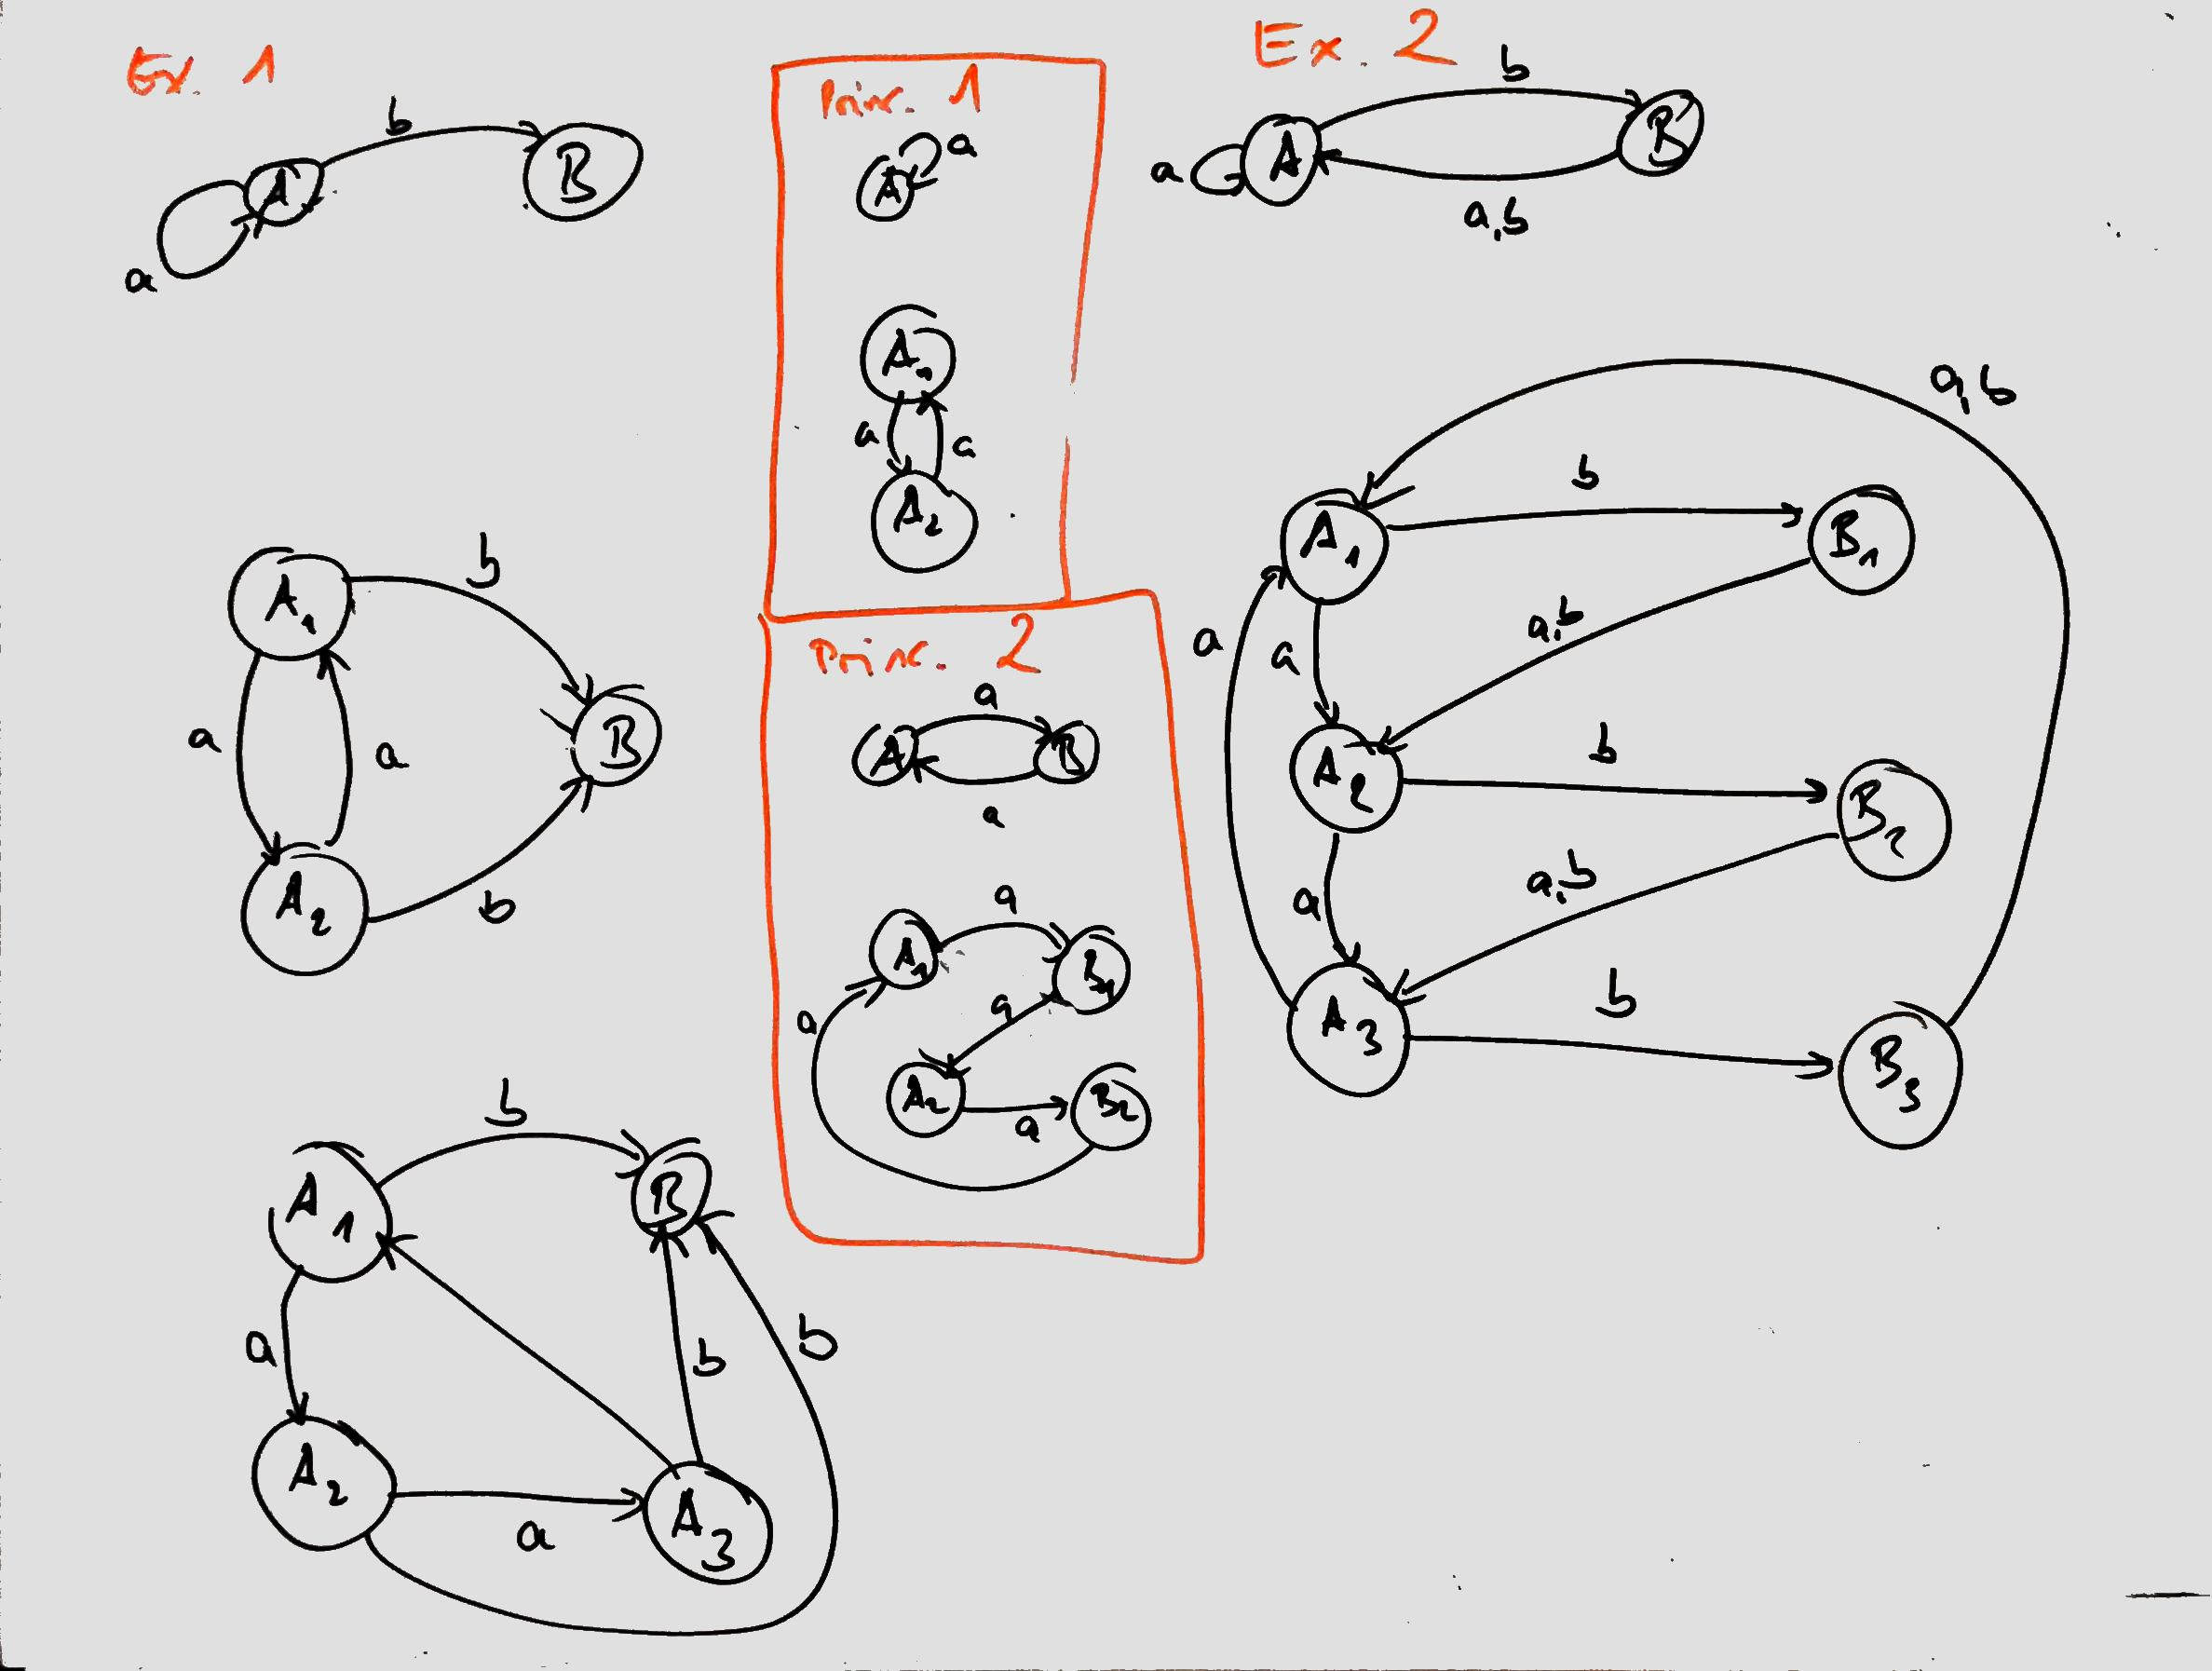
\includegraphics[width=0.9\textwidth]{figures/correctness/orchestration/cycle_elimination.jpg}\\
    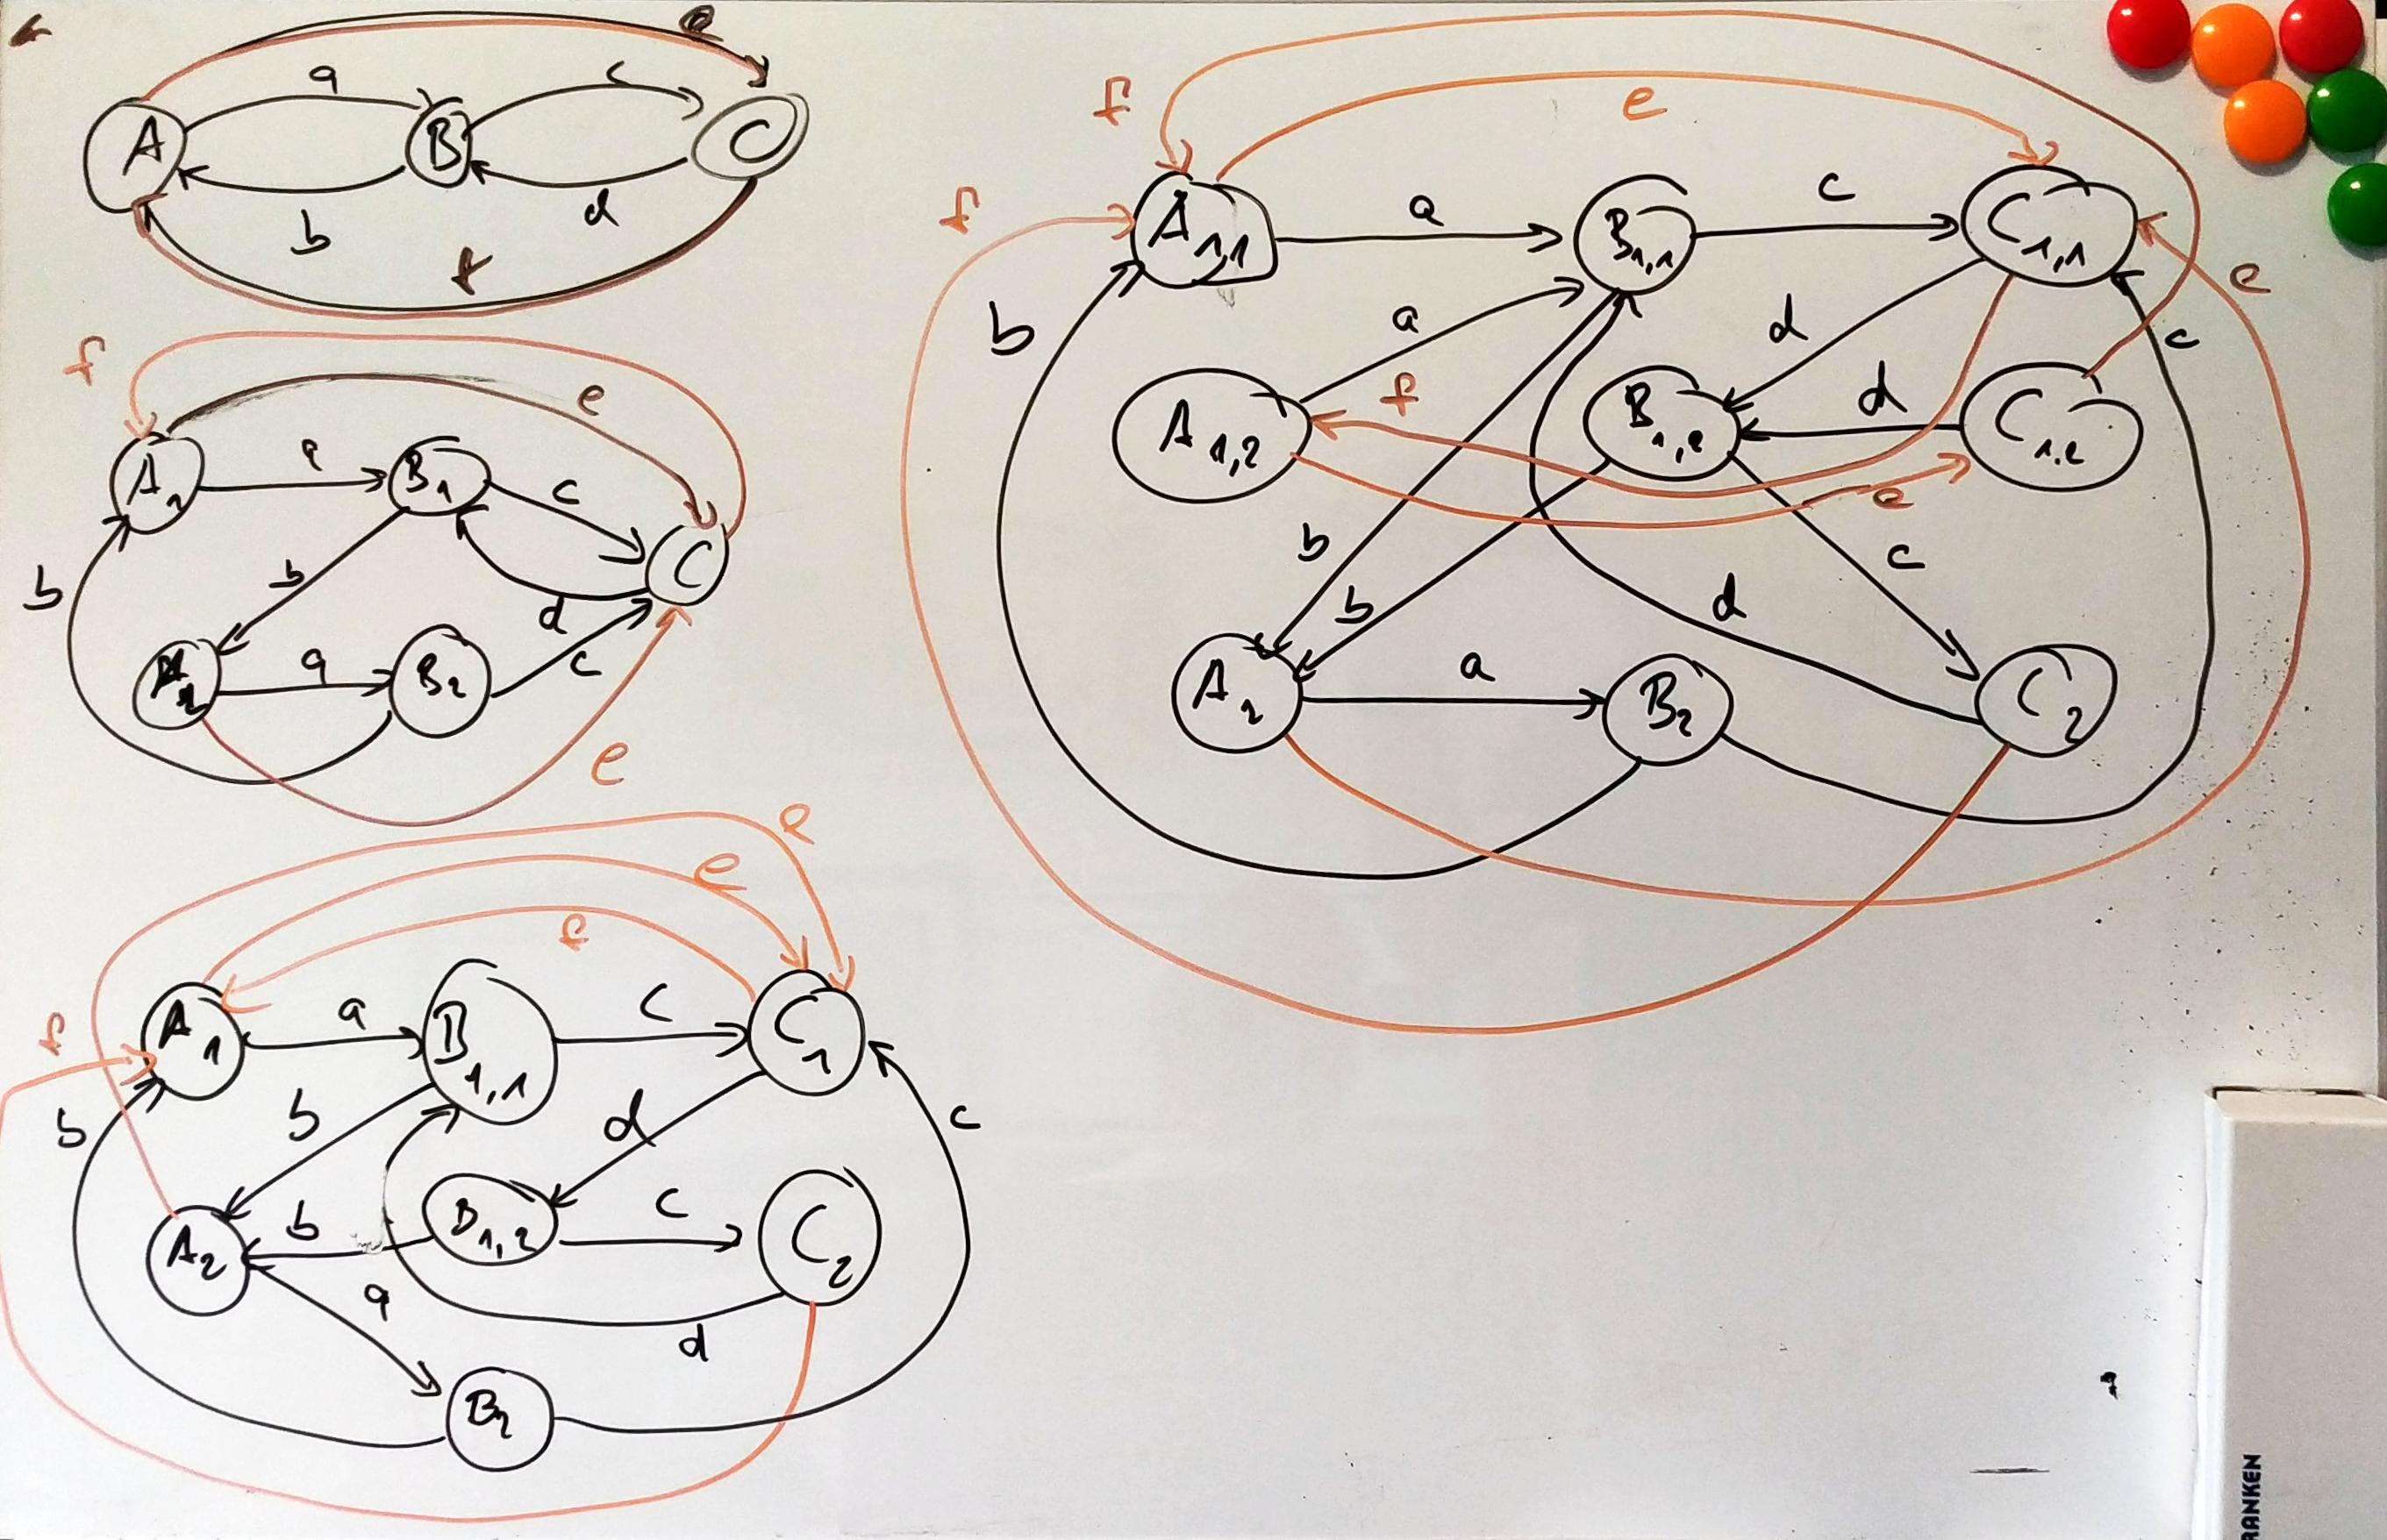
\includegraphics[width=0.9\textwidth]{figures/correctness/orchestration/cycle_elimination2.jpg}
    \caption[Cycle elimination in Turing machine transition functions]{Principles to eliminate cycles of length $\leq 2$ in transition function of a Turing machine and two application examples.}
    \label{fig:orchestration:cycle_elimination}
\end{figure}

\mnote{Assumptions for Turing machine}
Given a Turing machine $\TuringMachine$ over some alphabet $\Sigma$, we construct metamodels $\metamodeltuple{M}_{\TuringMachine}$ and a transformation network with a set of transformations $\transformationset{T}_{\TuringMachine}$, as well as initial models $\modeltuple{m}_{\TuringMachine, x} \in \metamodeltupleinstanceset{M_{\TuringMachine}}$ and changes $\changetuple{\metamodeltuple{M},\TuringMachine,x}$ for them for which a consistent orchestration exists if, and only if, $\TuringMachine$ halts on input $x \in \Sigma^*$.
Without loss of generality, we assume that the graph of the transition function of $\TuringMachine$ contains no cycles of length $\leq 2$.
This means that does not contain no self-loops, i.e., that the transition function always changes the state.
And that there is no cycle between two states.
This is without loss of generality, because cycles of these two lengths can be eliminated by duplicating states.
A self-loop can be eliminated by duplicating the state with a cycle of length $2$ between the duplicated states,  replicating all outgoing transitions for both states and let all ingoing transitions go to one of these two states.
Likewise, eliminating cycles of length $2$ can be achieved by duplicating both involved states and replacing the cycle of length $2$ by one of length $4$, replicating all outgoing transitions for all states and let all ingoing transitions go to one of the two states of each replicated one.
Inductively applying these duplication principles can eliminate all cycles of length $\leq 2$.
The two principles and the application to a scenario with self-loops as well as three states with pairwise cycles of length $2$ are depicted in \autoref{fig:orchestration:cycle_elimination}.

\mnote{Models representing states of Turing machine}
We construct models that consist of a timestamp, the tape content and the tape position.
With our formalism, we can, for example, encode this into a metamodel $\metamodel{M}{\TuringMachine}$ having one class with exactly these contents and models that do only contain one instance of that class.
For reasons of simplicity, we do not explicitly denote the according metamodel and denote a model $\model{m}{}$ as $\model{m}{} \in \mathbb{N}_0 \times \Sigma^* \times \mathbb{N}_0$.
We use one model for each state of the Turing machine and one transformation between each pair whose states have a transition between them.
To be able to identify the state which a model represents by its metamodel, we also assume one metamodel for each of the states, although they all look equal. Thus, we have $\metamodeltuple{M}_\TuringMachine = \tupled{\metamodel{M}{1, \TuringMachine}, \dots, \metamodel{M}{n, \TuringMachine}}$ with $n = \abs{Q_\TuringMachine}$ if we assume $Q_\TuringMachine = \setted{q_1, \dots, q_n}$ to be the set of states of $\TuringMachine$.
%Equivalently, we may also define $\abs{Q_\TuringMachine}$ metamodels with the same contents.
We define the following function that returns the state of the Turing machine represented by a metamodel:
\begin{align*}
     \function{Q} : %\setted{\metamodel{1,\TuringMachine}, \dots, \metamodel{n,\TuringMachine}} \rightarrow Q_\TuringMachine \\
     \metamodel{M}{i,\TuringMachine} & \mapsto q_i %\mathtext{with} \exists i \in \setted{1, \dots, n} : \model{m}{} \in \metamodelinstanceset{M}{i, \TuringMachine} \land q = q_i
\end{align*}
% We define the following function that returns the state of the Turing machine represented by a model:
% \begin{align*}
%      \function{Q} : \bigcup_{1 \leq i < n} \metamodelinstanceset{M}{i, \TuringMachine} & \rightarrow Q_\TuringMachine \\
%      \model{m}{} & \mapsto q \mathtext{with} \exists i \in \setted{1, \dots, n} : \model{m}{} \in \metamodelinstanceset{M}{i, \TuringMachine} \land q = q_i
% \end{align*}

\mnote{Transformations representing transitions of the Turing machine}
The transformations increment the timestamp, change the tape content and update the tape position according to the transition of $\TuringMachine$ if, and only if, the timestamp of one model is higher than the one of the other.
More formally, let $\Tr(q_1,q_2) \subseteq \Sigma \times \setted{-1,0,1} \times \Sigma$ be the transitions defined between the states $q_1 \in Q_\TuringMachine$ and $q_2 \in Q_\TuringMachine$ (with $-1$, $0$ and $1$ indicating the head movements \enquote{left}, \enquote{stay} and \enquote{right}). \todo{Visualize at an example}
We define a consistency preservation rule for the transformation between metamodels $\metamodel{M}{i, \TuringMachine}$ and $\metamodel{M}{k, \TuringMachine}$ realizing the transition between the represented states of $\TuringMachine$ as follows:
% {
% 	\newcommand{\shiftedcase}[1]{%
% 		$\begin{adjustbox}{Trim=1.7cm 0pt 0pt 0pt}$%
% 			#1%
% 		$\end{adjustbox}$
% 	}
% \begin{align*}
%     &
%     \consistencypreservationrule{}(\model{m}{1} = \tupled{\mathvariable{time}_{\model{m}{1}}, \mathvariable{cont}_{\model{m}{1}}, \mathvariable{pos}_{\model{m}{1}}}, \model{m}{2} = \tupled{\mathvariable{time}_{\model{m}{2}}, \mathvariable{cont}_{\model{m}{2}}, \mathvariable{pos}_{\model{m}{2}}}, \change{\metamodel{M}{1}}, \change{\metamodel{M}{2}}) \\
%     & \formulaskip
%     = (\change{\metamodel{M}{1}}', \change{\metamodel{M}{2}}')
% \end{align*}
\begin{align*}
    &
    \consistencypreservationrule{i,k}(\model{m}{i}, \model{m}{k}, \change{\metamodel{M}{i,\TuringMachine}}, \change{\metamodel{M}{k,\TuringMachine}}) = (\change{\metamodel{M}{i,\TuringMachine}}', \change{\metamodel{M}{k,\TuringMachine}}')
\end{align*}
with
\begin{align*}
    &
    \model{m}{i}' = \tupled{\mathvariable{time}_{\model{m}{i}'}, \sequence{\mathvariable{cont}_{\model{m}{i}'}}, \mathvariable{pos}_{\model{m}{i}'}} \equalsperdefinition \changetuple{\metamodel{M}{i,\TuringMachine}}(\model{m}{i}) \\
    &
    \model{m}{k}' = \tupled{\mathvariable{time}_{\model{m}{k}'}, \sequence{\mathvariable{cont}_{\model{m}{k}'}}, \mathvariable{pos}_{\model{m}{k}'}} \equalsperdefinition \changetuple{\metamodel{M}{k,\TuringMachine}}(\model{m}{k}) \\
    &
    \change{\metamodel{M}{i,\TuringMachine}}'(\model{m}{i}) = 
    \begin{cases}
        \tupled{\mathvariable{time}_{\model{m}{k}'} + 1, \mathvariable{cont}_{\model{m}{k}'}|_{\mathvariable{pos}_{\model{m}{k}'} \gets \mathvariable{repl}}, \mathvariable{pos}_{\model{m}{k}'} + \mathvariable{dir}}, \\
        \formulaskip\formulaskip 
            \text{if } \mathvariable{time}_{\model{m}{k}'} > \mathvariable{time}_{\model{m}{i}'} \\
        \formulaskip\formulaskip\formulaskip
            \land \exists \tupled{\sequenceindex{\mathvariable{cont}_{\model{m}{k}'}}{\mathvariable{pos}_{\model{m}{k}'}}, \mathvariable{dir},\mathvariable{repl}} \in \Tr(Q(\metamodel{M}{i,\TuringMachine}),Q(\metamodel{M}{k,\TuringMachine}))\\[.4em]
        \change{\metamodel{M}{i,\TuringMachine}}(\model{m}{i}'), \formulaskip 
        \text{else}
    \end{cases} \\
    &
    \change{\metamodel{M}{k,\TuringMachine}}'(\model{m}{k}) = 
    \begin{cases}
        \tupled{\mathvariable{time}_{\model{m}{i}'} + 1, \mathvariable{cont}_{\model{m}{i}'}|_{\mathvariable{pos}_{\model{m}{i}'} \gets \mathvariable{repl}}, \mathvariable{pos}_{\model{m}{i}'} + \mathvariable{dir}}, \\
        \formulaskip\formulaskip 
            \text{if } \mathvariable{time}_{\model{m}{i}'} > \mathvariable{time}_{\model{m}{k}'} \\
        \formulaskip\formulaskip\formulaskip
            \land \exists \tupled{\sequenceindex{\mathvariable{cont}_{\model{m}{i}'}}{\mathvariable{pos}_{\model{m}{i}'}}, \mathvariable{dir},\mathvariable{repl}} \in \Tr(Q(\metamodel{M}{i,\TuringMachine}),Q(\metamodel{M}{k,\TuringMachine}))\\[.4em]
        \change{\metamodel{M}{k,\TuringMachine}}(\model{m}{k}'), \formulaskip 
        \text{else}
    \end{cases}
\end{align*}

%\begin{multline*}  
% \forall \left(a,b\right)\in E: T_{\TuringMachine}\left(a,b\right)\left(\alpha\!\eqqcolon\!\left(t_a,w_a,p_a\right), \beta\!\eqqcolon\!\left(t_b,w_b,p_b\right)\right)\\
% 		=\begin{cases}%
% 			\left(\alpha,\left(t_a\! +\! 1,\, w_{a}|_{p_a\gets r},\,p_a\!+\!d\right)\right)  \\
% 			&\shiftedcase{\text{if }t_a > t_b\land\exists\,\left(w_{a}\left[p_a\right],d,r\right)\in\Tr\left(a,b\right)}\\[.4em]
% 			\left(\left(t_b\! +\! 1,\, w_{b}|_{p_b\gets r},\,p_b\!+\!d\right),\,\beta\right)   \\
% 			&\shiftedcase{\text{if }t_a < t_b\land\exists\,\left(w_{b}\left[p_b\right],d,r\right)\in\Tr\left(b,a\right)}\\[.4em]
% 			\left(\alpha, \beta\right)                                  &\shiftedcase{\text{else}}
% 		\end{cases}
% \end{multline*}
% }
where $\mathvariable{cont}|_{\mathvariable{pos} \gets \mathvariable{repl}} \equalsperdefinition \sequenceindex{\mathvariable{cont}}{0\:..\:\mathvariable{pos}-1} \cdot \mathvariable{repl} \cdot \sequenceindex{\mathvariable{cont}}{\mathvariable{pos}+1\:..\:|\mathvariable{cont}|-1}$.

\mnote{Consistency relations implied by consistency preservation rules}
The consistency relations are implicitly given by the fixed points of the consistency preservation rules.
For a consistency preservation rule $\consistencypreservationrule{i,k}$, we define:
\begin{align*}
    \consistencyrelation{CR}{i,k} = \setted{\model{m}{i}, \model{m}{k}} \in \metamodelinstanceset{M}{i,\TuringMachine} \times \metamodelinstanceset{M}{k,\TuringMachine} \mid \consistencypreservationrule{i,k}(\model{m}{i},\model{m}{k},\identitychange,\identitychange) = \tupled{\identitychange,\identitychange}
\end{align*} 
With this definition, each consistency preservation rule is correct, i.e., one application of it yields models that are consistent to its defined consistency relation, because due to the assumption that the transition function of $\TuringMachine$ does not contain cycles of length $\leq 2$, there may be no cyclic transition between the states which are represented by the models kept consistent by a single transformation.

\mnote{Transformation whenever transition between according states exists}
We denote the set of all transformations realizing the transitions of $\TuringMachine$ as $\transformationset{T}_{\TuringMachine}$, containing transformations $\transformation{t}_{i,k} = \tupled{\consistencyrelation{CR}{i,k},\consistencypreservationrule{i,k}}$ for all metamodel pairs $\tupled{\metamodel{M}{i,\TuringMachine},\metamodel{M}{k,\TuringMachine}}$, for which a transition between the represented states in $Q_\TuringMachine$ exists, i.e. $\Tr(Q(\metamodel{M}{i,\TuringMachine}),Q(\metamodel{M}{k,\TuringMachine})) \neq \emptyset$.

\mnote{Representation of Turing machine start state in models}
Let $s \in Q_{\TuringMachine}$ be the initial state of $\TuringMachine$. We set
\begin{align*}
    &
    \modeltuple{m}_{\TuringMachine, x} = \tupled{\model{m}{1,\TuringMachine,x}, \dots, \model{m}{n,\TuringMachine,x}} \\
    & \formulaskip\formulaskip\formulaskip
    \withmath \forall i \in \setted{1, \dots, n} : %\model{m}{\TuringMachine,x} \in \modeltuple{m}_{\TuringMachine, x} : \model{m}{\TuringMachine, x} = \tupled{0, \varepsilon, 0} \\
    \model{m}{i, \TuringMachine, x} = \tupled{0, \varepsilon, 0} \\
    %
    &
    \changetuple{\metamodeltuple{M},\TuringMachine,x} = \tupled{\change{\metamodel{M}{1},\TuringMachine,x}, \dots, \change{\metamodel{M}{n},\TuringMachine,x}} \withmath \\
    &
    \formulaskip\formulaskip\formulaskip
    \change{\metamodel{M}{i},\TuringMachine,x}(\model{m}{i}) = 
    \begin{cases}
        \tupled{1,x,0}, & \mathtextspacearound{if} Q(\model{m}{i}) = s\\
        \model{m}{i}, & \mathtextspacearound{else}
    \end{cases}
\end{align*}

\mnote{Auxiliary lemma for reduction of halting problem to orchestration problem}
We can show that for every Turing machine, this construction of a transformation network out of it solves the halting problem by construction if we are able to solve the orchestration problem.
First, we show an auxiliary lemma that proves that executing the transformations until all models are consistent terminates if, and only if, the according Turing machine halts.

\begin{lemma}[Turing Machine to Transformation Network Reduction]
    \label{lemma:turing_machine_construction}
    Executing the transformations of $\transformationset{T}_{\TuringMachine}$ for the models $\modeltuple{m}_{\TuringMachine,x}$ and changes $\changetuple{\metamodeltuple{M},\TuringMachine,x}$ until all models are consistent %no transformations modify the changes any more 
    terminates if, and only if, $\TuringMachine$ halts on input $x$.
	If executing the transformations terminates with the final changes $\changetuple{\metamodeltuple{M},f}$, then the model in $\modeltuple{m}_{f} = \changetuple{\metamodeltuple{M},f}(\modeltuple{m}_{\TuringMachine,x})$ with the highest timestamp contains $\TuringMachine(x)$ as tape content.
\end{lemma}
\begin{proof}
    Let $\changetuple{s}, s \in \mathbb{N}_0$ be the sequence of changes created while executing the transformations and let $\modeltuple{m}_{s} = \tupled{\model{m}{1,s}, \dots, \model{m}{n,s}}\equalsperdefinition \changetuple{s}(\modeltuple{m}_{\TuringMachine,x})$ be the state of the models after applying that change.
    Then we can see per induction over the model states $\modeltuple{m}_{s}$:
	\begin{longenumerate} %[1., left=0pt .. \parindent]
        \item 
            There is at most one transformation $\transformation{t}_{i,k} \in \transformationset{T}_{\TuringMachine}$, such that $\tupled{\model{m}{i,s},\model{m}{k,s}}$ is not consistent to $\transformation{t}_{i,k}$, i.e., $\tupled{\model{m}{i,s},\model{m}{k,s}} \not\in \consistencyrelation{CR}{i,k}$.
            This follows from the definition of $\TuringMachine$ and the last executed transformation.
            Let us, in contrary, assume there was a second transformation that could be executed. 
            We can longenumerate whether the transformation involves any of $\model{m}{i,s},\model{m}{k,s}$ or not.
            If that transformation involves any of these two models, then $\TuringMachine$ would have been non-deterministic, because each transformation realizes a transitions between the associated states of $\TuringMachine$.
            If that transformation involves none of these models, then one them must have been changed before, because otherwise they are consistent by construction of $\modeltuple{m}_{\TuringMachine,x}$.
            Let that changed model be $\model{m}{}'$.
            The transformation to which $\model{m}{}'$ and another model are inconsistent cannot be the one that was executed after $\model{m}{}'$ was changed, because its correctness ensures that the two are consistent afterwards.
            Again, due to $\TuringMachine$ being deterministic, there cannot be another transformation that needed to be executed after $\model{m}{}'$ was changed. Thus another model must have been changed later which led to the inconsistency. Then, however, the transformation would have needed to be applied because of the other changed model.
            Since another transformation was executed and again because of $\TuringMachine$ being deterministic, that inconsistency cannot occur, thus being a contradiction to the assumption.
            % If a model $\model{m}{h,s}$ is changed, then only one of the transformations involving $\model{m}{h,s}$ makes changes, as each of them realizes a the transitions of $\TuringMachine$ and if more than one of them could be executed, $\TuringMachine$ would have been non-deterministic.
            % Per induction, for the previously changed model there was also only one transformation that needed to be executed to restore consistency. If the models are still inconsistent after the transformation has been executed, then a change in the opposite direction must be necessary because of the changed timestamp, which must then be exactly $\transformation{t}_{i,k}$ because of $\TuringMachine$ being deterministic.
            % This inductively ensures that there is always at most one transformation that needs to be executed to restore consistency.
            %Note that there may be no transformation to execute if for the state of $\TuringMachine$ encoded in all current models no transition exists in $\Tr$, which can especially occur if a final state is reached.
            %% There is at most one edge \(\left(a,b\right)\in E\) whose transformation is inconsistent, i.e. \(\left(M_i\left(a\right),M_i\left(b\right)\right)\notin R_{T_{\TuringMachine}\left(a,b\right)}\).
			%% This follows from the definitions of \(\TuringMachine\) and the last executed transformation.
		 	%% Additionally, \(a=v\) or \(b=v\),
		 	%% because otherwise, there would have been two inconsistent transformations for \(M_{i-1}\).
		 	%% We assume without loss of generality \(a=v\).
        \item 
            There is exactly one model $(time,cont,pos) \equalsperdefinition \model{m}{h,s} \in \modeltuple{m}_{s}$ that has the highest timestamp $time$ of all models in $\modeltuple{m}_{s}$.
            This follows from the previous insight that there is always at most one transformation to which the models are not consistent and which thus can perform changes, and that this transformation involves the just changed model, which, per induction, has the highest timestamp of all models.
            Thus, this model must either be $\model{m}{i,s}$ or $\model{m}{k,s}$.
            We assume without loss of generality $\model{m}{h,s} = \model{m}{i,s}$.            
		 \item
            If a $\transformation{t}_{i,k}$ exists to which $\tupled{\model{m}{i,s},\model{m}{k,s}}$ is not consistent, then $\model{m}{k,s+1}$ %\(\left(a,b\right)\) exists, then \(m'\!\coloneqq\! M_{i+1}\left(b\right)\) 
            will contain the same tape content and the same tape position as would result if $\TuringMachine$ was executed one step from the state encoded in $\model{m}{i,s}$ with tape content $\mathvariable{cont}_s$ and tape position $\mathvariable{pos}_s$.
		 	Additionally, $\model{m}{k,s+1}$ will be the model with the highest timestamp of all models in $\modeltuple{m}_{s+1}$.
		 \item 
             $\modeltuple{m}_{s}$ is consistent to $\transformationset{T}_{\TuringMachine}$ and thus no further transformation can produce changes if, and only if, $\TuringMachine$ would halt in state $\model{m}{i,s}$ with tape content $\mathvariable{cont}_s$ and tape position $\mathvariable{pos}_s$.
             This is given by construction of the transformations, because a transformation can be executed if, and only if, the timestamp of the model is lower than the timestamp of a model to which a transformation is defined and if there is an according transition in $\Tr$ of $\TuringMachine$ and if.
             Since the timestamp of $\model{m}{i,s}$ is higher than the timestamp of all other models, a transformation can be executed if, and only if, there is an according transition of $\TuringMachine$, thus the execution of transformations terminates exactly when $\TuringMachine$ halts.
		 	\qedhere
	\end{longenumerate}
\end{proof}

\mnote{The orchestration proble is undecidable}
With this lemma, it is easy to see that we could decide the halting problem if we can decide whether a consistent orchestration for the transformation network construction from a Turing machine exists.
In consequence, the orchestration problem is undecidable.

\begin{theorem}[Orchestration Problem Undecidability] \label{theorem:orchestration_problem_undecidability}
    The orchestration problem is undecidable.
\end{theorem}
\begin{proof}
    We have given the constructive proof for \autoref{lemma:turing_machine_construction} that any Turing machine can be simulated by a transformation network such that a repeated execution of transformations finds consistent models of which one contains the resulting tape content of the Turing machine if, and only if, the Turing machine halts.
    Thus, if we could decide the orchestration problem, we could decide whether a consistent orchestration exists.Since the consistent orchestration for the given transformations is unique, as in each step there is always only one transformation that can be executed, knowing that a consistent orchestration exists means, according to \autoref{lemma:turing_machine_construction}, that we can decide whether $\TuringMachine$ halts, i.e., we could decide the halting problem.
\end{proof}

\mnote{An application function cannot be optimal}
According to \autoref{theorem:optimal_application_function_orchestration_problem}, we can only find an optimal application function if the orchestration problem is decidable.
Thus, we know that we cannot find such a function.

\begin{corollary}[Application Function Non-Optimality]
    \label{corollary:nooptimalapplication}
    Let $\appfunction{\orcfunction{\transformationset{T}}}$ be an application function. $\appfunction{\orcfunction{\transformationset{T}}}$ cannot be optimal.
\end{corollary}
\begin{proof}
    According to \autoref{theorem:optimal_application_function_orchestration_problem} an optimal application function can only be defined if a solution for the orchestration and orchestration existence problem, respectively, exists.
    Due to \autoref{theorem:orchestration_problem_undecidability}, we know that the problem is undecidable and thus an optimal application function cannot be defined.
\end{proof}

% \begin{lemma}[Optimal Application Function Decides Halting Problem]
%     \label{lemma:optimalapplicationturingmachine}
%     For any Turing machine $\TuringMachine$, we can construct metamodels $\metamodeltuple{M}_{\TuringMachine}$ and transformations $\transformationset{T}_{\TuringMachine}$ such that any optimal application application function yields consistent models for the models $\modeltuple{m}_{\TuringMachine,x}$ and changes $\changetuple{\metamodeltuple{M},\TuringMachine,x}$ if, and only if $\TuringMachine$ halts for input $x$.
% \end{lemma}
% \begin{proof}
%     We have given the constructive proof for \autoref{lemma:turingmachineconstruction} that any Turing machine can be simulated by a transformation network such that a repeated execution of transformations delivers the resulting tape content of the Turing machine as content of a model if, any only if, the Turing machine halts.
%     Since the construction ensures that in each step there only one transformation that can be executed because only one pair of models is inconsistent.
%     Thus, there is only one orchestration of the transformations for every input such that each of them performs changes and every application function has to execute the transformations in exactly that way.
% \end{proof}

% \begin{theorem}[Orchestration Problem Undecidability]
%     The orchestration problem is undecidable.
% \end{theorem}
% \begin{proof}
%     We have shown in \autoref{lemma:optimalapplicationturingmachine} that an optimal application function could decide the Halting problem for every Turing machine $\TuringMachine$ and every input.
%     Thus such a function cannot exist.
%     Due to \autoref{theorem:applicationfunctionsolveorchestrationproblem} an optimal application function solves the orchestration and orchestration existence problem, respectively.

%     In particular, an optimal application function finds that orchestration, because it yields consistent models.
%     Thus, implementing an optimal application function, which is able to decide whether a consistent orchestration exists, would solve the Halting problem.
% \end{proof}

% In particular, an optimal application function finds that orchestration, because it yields consistent models.
%     Thus, implementing an optimal application function, which is able to decide whether a consistent orchestration exists, would solve the Halting problem.

% \begin{lemma}
%     \label{lemma:networkfromturingmachine}
%     For any Turing machine $\TuringMachine$, we can construct metamodels $\metamodeltuple{M}$ and a transformation network $\transformationnetwork{N} = \tupled{\transformationset{T}, \appfunction{\orcfunction{}}}$ with an optimal application function $\appfunction{\orcfunction{}}$, such that $\TuringMachine$ halts for input $x$ if, and only if, for models $\modeltuple{m}_{x}$ and changes $\changetuple{\metamodeltuple{M},x}$ it is $\appfunction{\orcfunction{}}(\modeltuple{m}_{x}, \changetuple{\metamodeltuple{M},x}) \consistenttomath \transformationset{T}$.
% \end{lemma}
% \begin{proof}
%     \todo{Add proof with turing machine construction}
% \end{proof}

% \begin{theorem}
%     \label{theorem:nooptimalapplication}
%     Let $\appfunction{\orcfunction{}}$ be an application function. $\appfunction{\orcfunction{}}$ cannot be optimal.
% \end{theorem}
% \begin{proof}
%     An optimal $\appfunction{\orcfunction{}}$ returns consistent models whenever there is a consistent orchestration.
%     With such a function, we are able to decide whether such an orchestration exists or not.
%     \begin{align*}
%         \function{ExistsOrc}(\transformationset{T},\modeltuple{m},\changetuple{\metamodeltuple{M}}) =
%             \begin{cases}
%                 \textsc{true}, & \appfunction{\orcfunction{}}(\transformationset{T}, \modeltuple{m},\changetuple{\metamodeltuple{M}}) \consistenttomath \transformationset{T} \\
%                 \textsc{false}, & otherwise
%             \end{cases}
%     \end{align*}
%     $\function{ExistsOrc}$ returns \textsc{true} if, any only if, a consistent orchestration exists.
%     $\appfunction{\orcfunction{}}$ does, per definition, only return consistent models when there is an orchestration that yields them.
%     Additionally, it does always return consistent models when an orchestration that yields them exists, because it is optimal.
%     It follows from \autoref{lemma:networkfromturingmachine} that we can simulate a universal Turing machine with a transformation network in the sense that we can construct a transformation network whose application function delivers consistent models for a given input if, and only if, the Turing machine halts for corresponding inputs.
%     Calculating \function{ExistsOrc} would thus decide whether the Turing machine halts and thus decide the halting problem.
% \end{proof}

\mnote{Algorithm cannot terminate and be optimal}
From this corollary, it also follows that we cannot implement \function{Orchestrate} within the \function{Apply} algorithm in a way that it realizes an optimal application function and terminates always.

\begin{corollary}[Apply Algorithm Non-Optimality]
    \function{Apply} according to \autoref{algo:orchestration:application} cannot terminate and return consistent models whenever an orchestration exists that yields them for every possible input.
\end{corollary}
\begin{proof}
    If \function{Apply} always terminated and returned consistent models whenever there is an orchestration that yields them, it would implement an optimal application function. %and could be used to realize \function{ExistsOrc} from the proof of \autoref{theorem:nooptimalapplication}.
    According to \autoref{corollary:nooptimalapplication} an application function cannot be optimal.
\end{proof}

\mnote{Restrict expressiveness of transformations or accept conservativeness}
In consequence, we only have the two options to either restrict the expressiveness of the transformations such that they cannot be used to simulate a Turing machine anymore or to accept the situation that \function{Apply} may either not terminate in some cases or return $\bot$ although there is an orchestration that yields consistent models.
We call this behavior \emph{conservative}, because the algorithm does never return consistent models although there is no orchestration that yields them, but may not return consistent models in some cases in which actually such an orchestration existed.

\mnote{Undecidability does not necessarily prevent practical applicability}
Finally, just because the orchestration problem is undecidable does mean that this must be an essential problem for executing practical transformation networks.
Most programming languages are Turing-complete and are still used to develop functional and usable software.
Thus, it is important to know that, in general, the expressiveness of transformation networks makes the orchestration problem undecidable, but this must not mean that we cannot practically apply those networks.
We will thus especially focus on how to deal with this undecidability and conservatively approximate the problem.

\mnote{Discuss both options in the following}
%In the following, we first introduce alternation as a special case of non-termination that can be avoided by construction.
In the following, we discuss options to restrict transformations to make the orchestration problem solvable and finally conclude that this is not an option for solving the above discussed problem.
Afterwards, we discuss how we can realize \function{Apply} in a way that it always terminates and produces reasonable outputs.

% \begin{corollary}
%     The orchestration problem (see \autoref{def:orchestrationproblem}) is undecidable.
% \end{corollary}
% \begin{proof}
%     \todo{Add proof. Maybe this should be the theorem from the Turing machine. Then we follow insights to the algorithm from that.}
% \end{proof}
%Lemma: It is undecidable whether an orchestration exists for a given input.

%Theorem: We cannot guarantee termination of Algorithm, when we allow an arbitrary number of transformation execution. (combine with upper bound, see above/below)

% Consequence: Either we need to restrict transformations to make the problem decidable or we need to restrict the application function and allow it to return $\bot$ although a sequence returning consistency exists, thus, we need to deal with conservativeness.
% \textit{Weaker version:}
% Goal: Find a solution in as many cases as possible, abort in the others (conservatively). There are two approaches to achieve that: 
% 1. Reduce the number of cases in which there is no solution by adding assumptions to the relations and transformations (restrict input of app function)
% 2. Improve the ability to find a solution if it exists (improve capabilities of app function)
% Secondary goal: In cases, in which no solution is found, support the user in understanding why no solution was found.

%Since we find that we cannot guarantee to find an orchestration, we need to deal with the conservative case anyway. Thus, we can also deal with the conservative case for the second problem instead of requiring things from the transformation which may not be (easily) fulfillable.

% Conclude that we cannot guarantee termination for an optimal orchestration function


\subsection{Restriction of Transformation Networks}
\label{chap:orchestration:decidability:restriction}

\mnote{Restrictions either transformation-local or for complete network}
We have discussed that it is necessary to restrict the transformations as an input of the application function to avoid that it is undecidable whether a consistent orchestration of them exists for given models and changes.
Those restrictions can be at two levels:
\begin{properdescription}
    \item[Transformation:] Restrictions only concern the single transformation. Thus, if each transformation fulfills a specific property, the application function is able to decide whether a consistent orchestration exists.
    \item[Network:] Restrictions concern the complete network, i.e., the combination of transformations. Only a set of transformations can have an appropriate property that enables the application function to decide the orchestration problem, but not each transformation on its own.
\end{properdescription}

\mnote{Find that all restrictions are impractical}
Since we assume transformations to be developed and reused independently, restrictions to single transformations are of special interest.
It is, however, easy to see that it will unlikely be possible to define practical restrictions to single transformations that make the orchestration problem decidable.
We will see that even impractical restrictions do not make the problem decidable.
%Additionally, we discuss possible restrictions to complete networks.
%We discuss properties that obviously provide the ability to avoid divergence and alternation in the states of a network, namely monotony and confluence.
%Unfortunately, we will show that those restrictions are impractical.

% \todo{Maybe conflucence and monotony are rather restrictions of the application function (i.e. conservative operations) rather then restrictions of the transformation?}

% \begin{itemize}
%     \item Restrictions must, in the best case, be local to a transformation, i.e., they should be fulfillable without knowing with which other transformations the transformation shall be combined
%     \item Can this ever be the case?
% \end{itemize}

% \begin{itemize}
%     \item Discuss different restrictions we may apply to synchronizing transformations and networks
%     \item We conclude that none of them is practically
%     \item This does not mean that there is no restriction, but we were not able to find one
%     \item Maybe also discuss history-ignorance
% \end{itemize}

% Lösungsoptionen (Grad der Einschränkung an die Transformationen) --  überdeckt sich mit der Klassifizierung hierüber -> zusammenführen
% \begin{itemize}
%     \item Hohe Einschränkung: Jede beliebige Reihenfolge von ausgeführten Transformationen führt letztendlich zu einem korrekten Ergebnis (Fixpunktiteration -- Allquantifizierung) -- Hippokratie-Eigenschaft sorgt dafür, dass keine Transformation wieder etwas ändert, wenn Konsistenz bereits hergestellt ist.
%     Diese Eigenschaft ist in der Praxis möglicherweise zu strikt, da sie sehr starke Anforderungen an die Transformationen stellen müsste. Dafür wäre aber die Anwendungsfunktion trivial.
%     \item Mittlere Einschränkung: Es gibt eine Reihenfolge von ausgeführten Transformationen für jede Änderung die terminiert (Existenzquantifizierung) und die Ausführungsfunktion findet diese Reihenfolge.
%     Utopisch, dass die Anwendungsfunktion aus (potentiell sehr mächtigen) Transformationen die richtige Reihenfolge errechnen kann. Dafür aber (möglicherweise) weniger Anforderungen an die Transformationen (zumindest nicht mehr Anforderungen, denn die Allquantifizierung induziert die Existenzquantifizierung). Eine Funktion könnte dann zumindest nach best-effort versuchen, die richtige Reihenfolge zu finden und konservativ abbrechen, wenn sie diese nicht finden kann (also entweder konsistent terminieren oder terminieren mit der Aussage, dass es entweder keine solche Reihenfolge gibt -- bei relaxierten Anforderungen -- oder dass es sie nicht finden kann).  
%     \item Geringe Einschränkung: Es gibt potentiell keine Reihenfolge der Transformationen, die bei einer Änderung zu einer konsistenten Lösung kommt. Hier müsste die Ausführungsfunktion entsprechend einen Fehler ausgeben.
% \end{itemize}

%\subsection{Options in Consistency Relations}

\mnote{Consistency preservation rules may select contradictory options in consistency relations}
We have seen in the examples and the discussion in \autoref{chap:orchestration:problem:function_behavior} that an essential reason for the non-existence of a consistent orchestration is the existence of options within consistency relations.
This means that a condition element is allowed to correspond to to different condition elements to be considered consistent, like we have seen for the mapping of names in \autoref{fig:orchestration:no_orchestration}.
Different transformations can define different such options for specific elements, such that some of these options can never exist in globally consistent models, but only the ones that overlap between the consistency relations of all transformations can occur there.
Compatibility of the consistency relations ensures that there is at least one such element in the overlap of the consistency relations, because if there was no consistent tuple of models containing the condition element the relations would be considered incompatible.
Unfortunately, each transformation can only select one of these options to restore consistency when a condition element is added and if all transformations choose an element that is not in the overlap of the consistency relations, they will never find a consistent tuple of models.

\mnote{Reduce expressiveness by each condition element only in one consistency relation pair}
In consequence, an obvious option to reduce expressiveness of transformations in order to make the orchestration problem decidable by ensuring that a consistent orchestration does always exist would be to restrict consistency relations, such that each condition element is only allowed to occur in a single consistency relation pair of a consistency relation.
Thus, each condition element has a unique corresponding element to which it is considered consistent.
Then, the consistency preservation rules cannot select between different options to restore consistency and if the relations are compatible, all consistency relations relate elements in an equal way, thus the transformations must find exactly those elements.

\mnote{Consistency relation restriction does not solve the problem}
Although that approach will at least reduce the number of cases in which no consistent orchestration is found in our algorithm, there are still inputs for which no consistent orchestration exists.
Since we do not restrict the transformation in what they are allowed to do, they can perform arbitrary changes to restore consistency.
This especially includes that they may always returns changes that yield the same two models, which are consistent to that transformation but not to any models that can be delivered by the other transformations.
% Since we do not restrict the transformation in what they are allowed to do, they can perform arbitrary changes that restore consistency, such that alternations in the execution can occur.
% Consider three metamodels $\metamodel{A}, \metamodel{B}, \metamodel{C}$ with the following consistency relations and consistency preservation rules:
% \begin{align*}
%     &
%     \consistencyrelation{CR}{AB} = \setted{\tupled{\model{a}{1}, \model{b}{1}}, \tupled{\model{a}{2}, \model{b}{3}}, \tupled{\model{a}{3}, \model{b}{2}, \tupled{\model{a}{4}, \model{b}{4}} \\
%     &
%     \consistencypreservationrule{\consistencyrelation{AB}}(\model{a}, \model{b}, \change{\metamodel{A}}, \change{\metamodel{B}}) = \begin{cases}
%     \end{cases}
%     &
%     \consistencyrelation{CR}{BC} = \setted{\tupled{\model{b}{1}, \model{c}{1}}, \tupled{\model{b}{2}, \model{c}{3}}, \tupled{\model{b}{3}, \model{c}{2}, \tupled{\model{b}{4}, \model{c}{4}} \\
%     &
%     \consistencyrelation{CR}{AC} = \setted{\tupled{\model{a}{1}, \model{c}{1}}, \tupled{\model{a}{2}, \model{c}{3}}, \tupled{\model{a}{3}, \model{c}{2}, \tupled{\model{a}{4}, \model{c}{4}} \\
% \end{align*}

\mnote{Example with restriction but without consistent orchestration}
Let $\class{A}{}$, $\class{B}{}$, $\class{C}{}$ be three classes, each with one attribute $n$ storing a number.
We define the following metamodels, each only consisting of one of those classes, and consistency relations between them that define that for each element in one model a corresponding the others with the same value of $n$ has to exist.
These consistency relations are obviously compatible.
This is a further simplification of our running example that requires persons, residents and employees with the same names.
Additionally, we define consistency preservation rules, each of them delivering changes that always, i.e., for every input, yield the same models that only consist of one element with a specific value.
The resulting models are chosen in a way such that they are consistent to the according consistency relation, but not to any of the others.
\begin{align*}
    & 
    \metamodelinstanceset{M}{1} = \mathcal{P}(\instances{\class{A}{}}), %\\
    %& 
    \metamodelinstanceset{M}{2} = \mathcal{P}(\instances{\class{B}{}}), %\\
    %& 
    \metamodelinstanceset{M}{3} = \mathcal{P}(\instances{\class{C}{}}) \\[1em]
    &
    \consistencyrelation{CR}{12} = \setted{\tupled{a,b} \in \instances{\class{A}{}} \times \instances{\class{B}{}} \mid a.n = b.n}, \consistencyrelationset{CR}_{12} = \setted{\consistencyrelation{CR}{12}, \consistencyrelation{CR}{12}^T} \\
    &
    \consistencypreservationrule{\consistencyrelationset{CR}_{12}}(\model{m}{1}, \model{m}{2}, \change{\metamodel{M}{1}}, \change{\metamodel{M}{2}}) = (\change{\metamodel{M}{1}}', \change{\metamodel{M}{2}}') \\
    & \formulaskip
        \withmath \change{\metamodel{M}{1}}'(\model{m}{1}) = \setted{a \in \instances{\class{A}{}} \mid a.n = 1} \land \change{\metamodel{M}{2}}'(\model{m}{2}) = \setted{b \in \instances{\class{B}{}} \mid b.n = 1} \\[1em]
    &
    \consistencyrelation{CR}{13} = \setted{\tupled{a,c} \in \instances{\class{A}{}} \times \instances{\class{C}{}} \mid a.n = c.n}, \consistencyrelationset{CR}_{13} = \setted{\consistencyrelation{CR}{13}, \consistencyrelation{CR}{13}^T} \\
    &
    \consistencypreservationrule{\consistencyrelationset{CR}_{13}}(\model{m}{1}, \model{m}{2}, \change{\metamodel{M}{1}}, \change{\metamodel{M}{3}}) = (\change{\metamodel{M}{1}}', \change{\metamodel{M}{3}}') \\
    & \formulaskip
        \withmath \change{\metamodel{M}{1}}'(\model{m}{1}) = \setted{a \in \instances{\class{A}{}} \mid a.n = 2} \land \change{\metamodel{M}{3}}'(\model{m}{3}) = \setted{b \in \instances{\class{C}{}} \mid c.n = 2} \\[1em]
    &
    \consistencyrelation{CR}{23} = \setted{\tupled{b,c} \in \instances{\class{B}{}} \times \instances{\class{C}{}} \mid b.n = c.n}, \consistencyrelationset{CR}_{23} = \setted{\consistencyrelation{CR}{23}, \consistencyrelation{CR}{23}^T} \\
    &
    \consistencypreservationrule{\consistencyrelationset{CR}_{23}}(\model{m}{2}, \model{m}{3}, \change{\metamodel{M}{2}}, \change{\metamodel{M}{3}}) = (\change{\metamodel{M}{2}}', \change{\metamodel{M}{3}}') \\
    & \formulaskip
        \withmath \change{\metamodel{M}{2}}'(\model{m}{3}) = \setted{b \in \instances{\class{B}{}} \mid b.n = 3} \land \change{\metamodel{M}{3}}'(\model{m}{3}) = \setted{c \in \instances{\class{C}{}} \mid c.n = 3}
\end{align*}

\mnote{Consistency preservation rules always yield models not consistent to other relations}
The given consistency relations are compatible, they contain each condition element only in one consistency relation pair, and the consistency preservation rules are correct, as their result is consistent to the consistency relation.
Still, there is no consistent orchestration of the transformation for any input that is not yet consistent.
This is because the consistency preservation rules always produce models that are not consistent to the consistency relations between the other models.

\mnote{Exemplary consistency preservation rules perform unreasonable changes}
One might argue that the defined consistency preservation rules are highly unreasonable and will never occur in that way in practice.
We would probably assume the consistency preservation rules to preserve the input models and changes in some way instead of returning models that are completely unrelated with the input.
However, we not yet have an appropriate notion for that.
Some were on transformations, such as \cite{cheney2017LeastChangeBx-JOT,macedo2016alloy}, proposes a notion of \emph{least change} to ensure that transformations do not perform arbitrary unrelated changes, which could exclude that situations.

\mnote{Restriction of consistency relations is impractical}
Although the given example is rather artificial and although there might be the additional property of least change, which could further reduce the cases in which no consistent orchestration exists, the essential drawback is that these restrictions are not reasonable.
Allowing a condition element to occur in multiple consistency relation pairs is essential, because options for elements to considered is necessary, especially if there is a gap in the abstraction of two related metamodels.
For example, a UML class needs to be able to correspond to all Java classes that provide different implementations of that class.
Requiring that there is exactly one Java class that is considered consistent to a UML class is obviously not applicable in practice, thus this restriction would make the consistency notion useless.

\mnote{Least change property does even not solve the problem}
If we, instead, only require some notion of least change, such as that only elements are changed which are involved in a violated consistency relation, this does also not solve the problem.
In the example in \autoref{fig:orchestration:no_orchestration}, relating the names of employees, residents and persons, we have defined consistency preservation rules that only require changes to elements that actually violate consistency.
Nevertheless, we have shown that for these consistency preservation rules only specific orchestrations are consistent and that with some modification even no consistent orchestration exists.

\mnote{Unlikely to find practical restrictions that solve the problem}
In consequence, we found that even a well-defined restriction that is too strong to be applied in practice still cannot ensure that a consistent orchestration exists for possible every input, even if the examples with used to show that on are rather artificial.
Although this does not serve as a proof for the impossibility for find a suitable restriction that solves the orchestration problem, which is even impossible because there is no unique notion of what an acceptable restriction would be, the investigated case shows that it is unlikely to find practical restrictions that solve the problem, if even impractical restrictions do not solve it.

% Es kann z.B. sein, dass ein Element a ein Element b braucht. Eine andere Transformation braucht zwei as und dafür ein (oder zwei) c. Dann ist (a,b) konsistent und es ist auch kompatibel, weil es mit dem a ein Modell gibt in dem es konsistent ist, nämlich das mit dem zweiten a, aber das Modell mit einem a ist nur lokal konsistent. Wenn das nun immer von der Transformation ausgewählt wird, findet man nie einen konsistenten Zustand.

% - We have seen that selection of options is a problem that leads to the non-existence of orchestrations.
% - Intended solution: Each object may only have one corresponding element. Then if the object exists, exactly one other has to exist. This ensure that for any model a there is only exactly one consistent b.
% It can, however, be that a1, b1 and c1 are consistent and a4, b4 and c4 are, but only (a2, b3), (a3, b2), (a2, c3), (a3, c2), (b2, c3), (c3, b2) are consistent. 
% The relations may still be compatible, because for example (a2, b3, a4), (a3, b2, a5) and so ond could be consistent.
% Since we have no requirements such as a least change requirement, the transformation may, for every input, return one of the last pairs, although this actually does not make any sense.
% Then the transformations do only alternate between those models.
% This seems to be a rather theoretical consideration, because transformations will usually not perform arbitrary unreasonable changes, such as always returning the same models.
% However, even if we found that we can define an additional property, such as least change, such that requiring each object to only have one corresponding element in the consistency relations together with that property, then still the latter requirement is impractical, as usually an element can correspond to different others.
% At least in the case when consistency relations gap abstraction levels, this is necessary.
% For example, a UML class needs to be able to correspond to a Java class with any implementation of its bodies. Restricting it to only one is not practical.

% Although the restriction of relations is already an impractical restriction, it does still not solve the problem.
% Thus it is unlikely to find restrictions that are practical and solve the problem, although, for sure, it is not formally proven.

% Even some notion of least change that ensure that only elements are changed which are involved in any violated consistency relations will not be sufficient, as the example in \autoref{fig:orchestration:no_orchestration} has shown.
% There, only elements that are involved in the violated consistency relations are changed.
%One might argue that in that example the consistency relations contain pairs of elements that can never be created by the consistency preservation rules and thus should not be part of the consistency relations.
%Gegenargument: Es gibt oft unendlich viele Paare (z.B. alle Implementierung einer Java Klasse mit einer UML-Klasse. Wenn auf der UML-Seite auch noch ein Freiheitsgrad ist, dann wird jede UML-Instanz der Klasse auf eine Standard Java-Klasse abgebildet und jede Java-Klasse auf eine Standard UML-Klasse, aber die Zusatzinformationen kommen erst durch manuellen Anreicherung dazu und sind dadurch vorhanden, aber nicht durch die Transformation)


\subsection{Confluence in Transformation Networks}
%\todo{Zeigen: Konfluenz führt zu Konvergenz. Aber konfluenz ist zu starke Anforderung, außerdem heißt Konvergenz, dass egal welche Reihenfolge der Transformationen man wählt am Ende immer das gleiche Ergebnis rauskommt. Das muss aber nicht so sein. Gebe Beispiel mit groß klein Schreibung, wo je nach Reihe folge verschieden elosungen rauskommen}
%\todo{Diss: Konvergenz einführen, hinreichende Eigenschaft? Notwendige Eigenschaft?}
%\todo{Discuss confluence and convergence!}

\begin{figure}
    \centering
    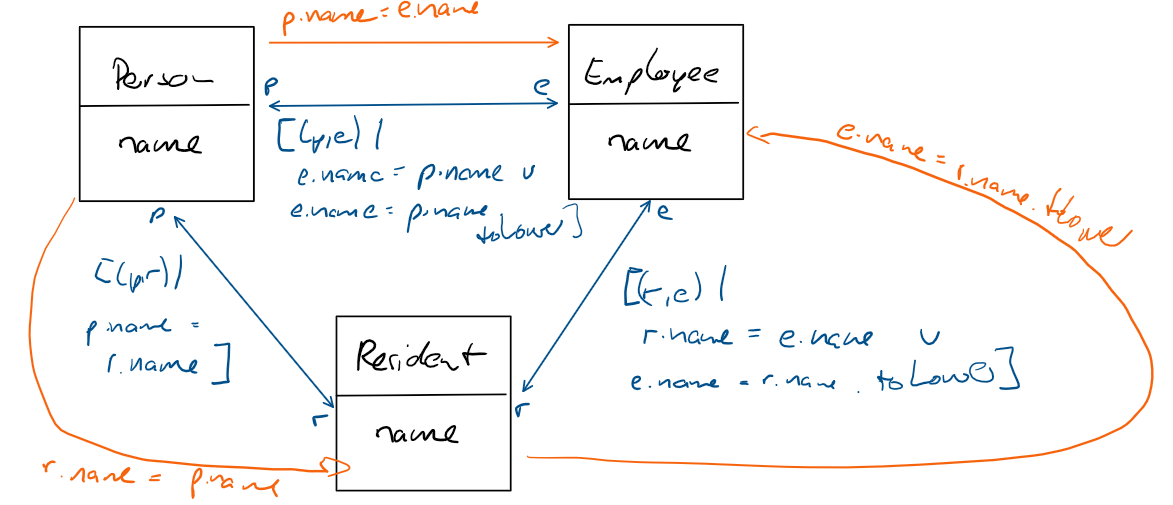
\includegraphics[width=\textwidth]{figures/correctness/orchestration/confluence.png}
    \caption[Confluence of transformations]{Counterexample for the practicality of confluence.}
    \label{fig:orchestration:confluence}
\end{figure}

\mnote{Confluence ensures that any consistent orchestration yields same result}
Confluence is an even stronger requirement than the existence of an optimal orchestration.
In literature~\cite{stevens2020BidirectionalTransformationLarge-SoSym}, confluence in a transformation network is described as the property that for given models and changes a consistent orchestration exists and that two consistent orchestrations for the same input always yield the same models.
Thus, executing transformations in any order such that the result is consistent will deliver the same result.
It is, however, easy to see that this is an impractical requirement.

\mnote{Counterexample for confluence}
In the example depicted in \autoref{fig:orchestration:confluence}, derived from the running example, three consistency relations expect for each person, employee and resident two corresponding others to exist.
They need to have the same name or, in case of the relations between persons and employees, as well as between residents and employees, the employee may have the same name in lower case.
The consistency preservation rule between persons and employees ensures that an employee with the same name exists, whereas the one between residents and employees ensures that an employee with the name in lower case exists.
Whenever a person is added, two consistent orchestrations can be distinguished.
First, the transformation between persons and employees can be executed, either followed or preceded by the one between persons and residents. Then all elements have the same name.
The models are also consistent to the relation between residents and employees, because the relation allows the names to be equal.
Second, the transformation between persons and residents can be executed, followed by the one between residents and employees.
Then the employee has the name in lower case, but still this is consistent to the relation between persons and employees.

\mnote{Confluence generally accepted as impractical}
Apart from that artificial example, such a situation can always occur if transformations have different options for elements to be consistent.
If there is not a single element that is in the overlap of consistent elements between all transformations, the result may be any of the elements in the overlap.
And the result may depend on which transformation made the first selection that fell into the overlap.
Finally, \textcite[p. 14]{stevens2020BidirectionalTransformationLarge-SoSym} also states explicitly that a network will only be confluent under very specific circumstances.

% Another intuitive notion of confluence would require that information flows together in a compatible way, i.e., the execution of a transformation does not violate consistency to other adjacent transformations.
% Formally this can be described as: A network is confluent when in every cycle of transformations t1,...tn the execution t1...ti-1 and tn,...,ti for any i leads to the same changes in the network.
% This means it does not matter in which order two transformations propagating information to the same model are executed.
% This, in consequence, means that the execution of a transformation cycles always yields models that are consistent to all transformations. Although two transformations affected the same model, consistency to the earlier executed one is not destroyed again.
% Finally, this reduces to the situation that executing each transformation once restores consistency to all transformations, which is, as we have seen, impractical.



\section{Conservative Approximation of the Orchestration Problem}

\mnote{Optimal orchestration cannot be achieved}
In the preceding section, we have proven that the orchestration problem is undecidable and we have discussed that it is unlikely to restrict the problem in a way such that it becomes decidable.
In consequence, we cannot achieve optimality of an orchestration and application function, which results in an 
algorithm that does not return optimal results and, depending on its implementation, does not terminate.
Since the algorithm cannot return optimal results anyway, termination can at least be achieved by introducing an artificial upper bound for the number of transformation applications.
This potentially prevents the algorithm even further from finding consistent orchestrations.

\mnote{Gradual optimality notion and approaches to improve it}
Based on those previous insights, we assume in this section that the orchestration problem cannot be restricted such that it becomes decidable.
We accept that any application function and any algorithm that realizes it will only realize a conservative approximation of the orchestration problem.
This means that it may only return consistent models delivered by a consistent orchestration, but it may not find a consistent orchestration although it exists.
In this case, we say that the function or algorithm, respectively, delivers \emph{false negatives} but no \emph{false positives} and call it \emph{conservative}.
We investigate how we can define optimality of the application function in gradual rather than a binary way, which is supposed to indicate how likely it is that it finds a consistent orchestration.
We then follow the goal of finding means to systematically improve optimality.
Since there are always cases in which the algorithm does not find a consistent orchestration, we propose an algorithm that is supposed to help identifying the reasons for failing in such cases in the subsequent section.

% \begin{itemize}
%     \item We conclude that we need to deal with the situation of undecidability. In consequence, orchestration must operate conservatively, i.e., we cannot assume to always find a solution, but if find it, it must be consistent.
%     \item One approach could be to reduce conservativeness. But even if we reduced conservativeness, we would not be able to completely eliminate it and thus have to deal with the situation that the strategy does not find a solution although it may exist.
%     \item We thus propose an approach that helps to identify the reason when the strategy is in the conservative case, i.e., not able to find a solution although it exists.
% \end{itemize}

%We found that we cannot achieve optimality (undecidability) for arbitrary transformations, we cannot restrict transformation such that we achieve decidability and thus optimality.
%So, we need to deal with situation can we cannot resolve all networks.
%Conclude: Conservativeness rather than correctness or achieving optimality (but improving the latter one)

% \mnote{Achieving a correct application function}
% The definition of the application function basically ensures that the function either returns $\bot$ or executes the \modellevelconsistencypreservationrules given by the orchestration function to retrieve a changes tuple of models.
% It is considered \emph{correct} if it ensures that its result is either $\bot$ or a consistent model tuple by executing the \modellevelconsistencypreservationrules given by the orchestration function.
% % A correct application function thus has to ensure that its result is either $\bot$ or a consistent model tuple by executing the \modellevelconsistencypreservationrules given by the orchestration function.
% In consequence, the application function can be realized by simply executing the result of the orchestration function and check whether the resulting model tuple is consistent or not and return an appropriate result.
% Such a realization is generic and does not depend on the actual consistency preservation rules and orchestration function but represents a generic behavior.
% Additionally, this gives an implementation of that function the ability to present a faulty result to the user, which eases finding out why no consistent state was reached.

% \mnote{Correctness is not crucial}
% Finally, correctness is not crucial, because correctness can easily be achieved by performing any execution of transformations and just ensuring that we terminate at some point in time and then decide whether the resulting models are consistent or not and appropriately deliver the result.

% \mnote{How to define an orchestration function that is as optimal as possible?}
% The remaining difficulty is how to define an orchestration function that fulfills the definition, i.e., to find a finite sequence of transformations, and also one that improves optimality, as an \emph{optimal} function can never be given.
% Although the definition of the orchestration function proposes a closed description of that function, in practice such a function will not have a closed form but will be realized as an algorithm that dynamically decides which transformation to execute next.
% Therefore the arising problem is that the length of the sequence to execute is not known a priori. Therefore, we need some abortion criterion. When a consistent result is found, this criterion is easy. But since we do not know whether a sequence exist, we need an abortion criterion that is reasonable and does not cut off the process although a consistent solution could be found, thus reducing optimality.
% A simple realization for that algorithm to deliver a finite sequence of transformations would be to define a fixed termination criterion, such as a specific number of transformation executions. However, there is no upper bound for the number of executed transformations necessary to achieve consistency. Still, a fixed number (even 0) could be defined for the number of executed transformations to fulfill the definition. Hence, optimality would be 0 then as a consistent result is never reached. We therefore discuss in the following how to define an appropriate orchestration function and how to optimize it.


\subsection{Systematic Improvement of Optimality}
\label{chap:orchestration:conservative:improvement}

%\subsection{A Gradual Notion of Optimality}
%\subsection{Reducing Conservativeness}

%Due to Turing-completeness of the network this would mean that the orchestration function can decide whether a Turing machine halts, which is proven impossible.
%Thus, our only goal can be to achieve optimality as far as possible in terms of reducing the degree of conservativeness, i.e., reduce the cases in which no sequence is found although it exists.

\mnote{Gradual notion of optimality}
Since no optimal application function can be achieved, we can at least define a gradual notion of optimality.
It indicates for how many inputs of models and changes the application function is able to return consistent models in comparison to the number of cases in which a consistent orchestration exists at all.
This can be seen as a fitness function for the optimality $\function{Opt}$ of an application function:
\begin{align*}
    &
    \function{Opt}(\appfunction{\orcfunction{\transformationset{T}}}) \\
    &\formulaskip
    = \frac{
        \abs{\setted{%\modeltuple{m} \in \metamodeltupleinstanceset{M},\changetuple{\metamodeltuple{M}} \in \changeuniverse{\metamodeltuple{M}}} 
        \tupled{\modeltuple{m},\changetuple{\metamodeltuple{M}}} \mid \appfunction{\orcfunction{\transformationset{T}}}(\modeltuple{m}, \changetuple{\metamodeltuple{M}}) \mathtext{is consistent to} \transformationset{T}}}
    }{
        \abs{\setted{\tupled{\modeltuple{m},\changetuple{\metamodeltuple{M}}} \mid \mathtext{consistent orchestration of} \transformationset{T} \mathtext{exists for} \tupled{\modeltuple{m}, \changetuple{\metamodeltuple{M}}}}}
    }
\end{align*}

\mnote{Concrete optimality values are not relevant}
In fact, both the numerator as well as the denominator will usually have infinite values, as there is an infinite number of possible models and changes to them.
It does, however, not matter for us what the actual optimality value of an application function is.
The purpose of the formula is only to explicitly state the influencing factors of optimality to be able to discuss its systematic improvement.

\mnote{Probability for finding correct orchestration by general random application function}
Obviously, we may only improve the numerator to improve optimality, because the denominator, i.e., the number of cases in which consistent orchestrations exist, depends only on the transformations and not the application function.
%is, first, not easy to achieve, and, second, may also reduce the number of cases in which a consistent orchestration is found.
How to improve the numerator highly depends on the concrete implemented application and orchestration functions.
For the most general case, let us assume that we have an application function $\appfunction{\orcfunction{\transformationset{T}}}$ whose orchestration function randomly tries any orchestration, i.e., it selects one of all possible orchestrations according to an equal distribution.
So we consider the following event $E_{\modeltuple{m},\changetuple{\metamodeltuple{M}}}$:
\begin{align*}
    &
    E_{\modeltuple{m},\changetuple{\metamodeltuple{M}}}: \appfunction{\orcfunction{\transformationset{T}}}(\modeltuple{m}, \changetuple{\metamodeltuple{M}}) \mathtext{is consistent to} \transformationset{T}
\end{align*}
The probability that this event occurs is given by the ratio between the number of consistent orchestrations for that input and the number of all orchestrations:
\begin{align*}
    &
    P(E_{\modeltuple{m},\changetuple{\metamodeltuple{M}}}) = \frac{
        \abs{\setted{\sequence{\transformation{t}} \in \transformationset{T}^{< \mathbb{N}} \mid \sequence{\transformation{t}} \mathtext{is consistent orchestration for} \tupled{\modeltuple{m}, \changetuple{\metamodeltuple{M}}}}}
    }{
        \abs{\transformationset{T}^{< \mathbb{N}}}
    }
\end{align*}
Here, the denominator is the size of what we previously introduced as the problem space $P = \abs{\transformationset{T}^{< \mathbb{N}}}$ containing all possible orchestrations, and the numerator is the size of what we previously introduced as the solution space $S_{i} = \abs{\setted{\sequence{\transformation{t}} \in \transformationset{T}^{< \mathbb{N}} \mid \sequence{\transformation{t}} \mathtext{is consistent orchestration for} \tupled{\modeltuple{m}, \changetuple{\metamodeltuple{M}}}}}$, which contains all consistent orchestrations for for an input of models and changes.

\mnote{Expected value for finding a consistent orchestration}
So we can introduce a stochastic variable $AppCons_{\modeltuple{m},\changetuple{\metamodeltuple{M}}}$, which assigns the values $0$ and $1$ to the events $E_{\modeltuple{m},\changetuple{\metamodeltuple{M}}}$ and its complementary:
\begin{align*}
    AppCons_{\modeltuple{m},\changetuple{\metamodeltuple{M}}}(\omega) = \begin{cases}
        0, & \omega = \appfunction{\orcfunction{\transformationset{T}}}(\modeltuple{m}, \changetuple{\metamodeltuple{M}}) \mathtext{is not consistent to} \transformationset{T} \\
        1, & \omega = \appfunction{\orcfunction{\transformationset{T}}}(\modeltuple{m}, \changetuple{\metamodeltuple{M}}) \mathtext{is consistent to} \transformationset{T}
    \end{cases}
\end{align*}
The expected value of this variable is then equal to the event $E_{\modeltuple{m},\changetuple{\metamodeltuple{M}}}$ to occur:
\begin{align*}
    \mu(AppCons_{\modeltuple{m},\changetuple{\metamodeltuple{M}}}) = P(AppCons_{\modeltuple{m},\changetuple{\metamodeltuple{M}}} = 1) = P(E_{\modeltuple{m},\changetuple{\metamodeltuple{M}}})
\end{align*}

\mnote{Number of found consistent orchestration is sum of expected values}
For an application function that chooses a random orchestration, we can thus express the numerator of $\function{Opt}(\appfunction{\orcfunction{\transformationset{T}}})$ as the sum of expected values of the stochastic variables for all possible inputs.
\begin{align*}
    &
    \abs{\setted{\tupled{\modeltuple{m},\changetuple{\metamodeltuple{M}}} \mid \appfunction{\orcfunction{\transformationset{T}}}(\modeltuple{m}, \changetuple{\metamodeltuple{M}}) \mathtext{is consistent to} \transformationset{T}}} = \sum_{\modeltuple{m},\changetuple{\metamodeltuple{M}}} \mu(AppCons_{\modeltuple{m},\changetuple{\metamodeltuple{M}}}) \\
    & \formulaskip
    = \frac{
        \sum_{\modeltuple{m},\changetuple{\metamodeltuple{M}}} \abs{\setted{\sequence{\transformation{t}} \in \transformationset{T}^{< \mathbb{N}} \mid \sequence{\transformation{t}} \mathtext{is consistent orchestration for} \tupled{\modeltuple{m}, \changetuple{\metamodeltuple{M}}}}}
    }{
        \abs{\transformationset{T}^{< \mathbb{N}}}
    }
\end{align*}

\mnote{Probability to find consistent orchestration improvable by reducing number of possibily considered orchestrations}
Thus, if we can improve $P(E_{\modeltuple{m},\changetuple{\metamodeltuple{M}}})$, we also improve optimality, even if orchestrations are chosen randomly.
We can improve that probability by either improving the number of consistent orchestrations or by reducing the number of possibly considered orchestrations.
The number of consistent orchestrations can only be influenced by requirements to the transformations.
For example, the requirement of consistency relations to be compatible improves this values, as we have shown by example in \autoref{chap:compatibility}.
In the following we discuss how we can reduce the number of possibly considered orchestrations while not reducing the number of consistent orchestrations, thus improving the probability of the application function to find a consistent orchestration and thus improving optimality.

\begin{figure}
    \centering
    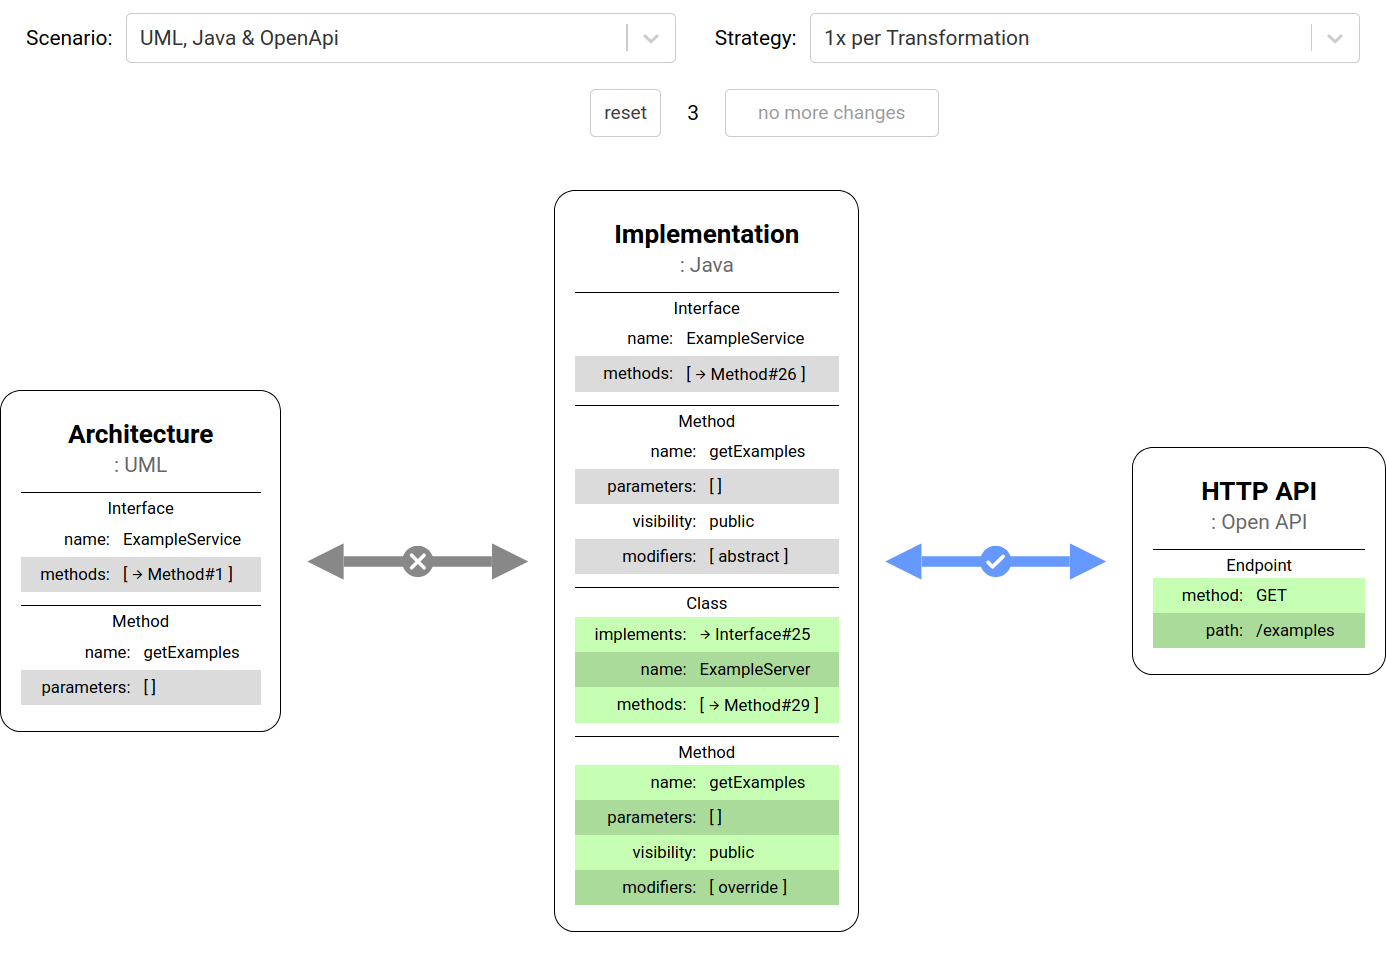
\includegraphics[width=0.8\textwidth]{figures/correctness/orchestration/simulator_screenshot.png}
    \caption[Screenshot of the transformation network simulator]{Screenshot of a network of for an architecture specification, its implementation and an API specification in OpenAPI, which requires multiple execution of the same transformation, developed in the transformation network simulator~\cite{orchestrationSimulator}.}
    \label{fig:orchestration:simulator}
\end{figure}

\mnote{No strategy that improves ability to find consistent orchestration}
The application function can, for sure, contain more intelligent logic for determining an orchestration beyond the random selection of an orchestration to improve the number of cases in which it finds a consistent orchestration.
By implementing further mechanisms to make a reasonable selection, the possibility to find a consistent orchestration may be further improved.
We investigated different orchestration strategies, such as the depth-first or breadth-first propagation of changes, and analyzed them with a simulator developed specifically for that purpose, which is available at GitHub~\cite{orchestrationSimulator}.
An example of a scenario showing the necessity to execute transformation more than once that we implemented in the simulator is depicted in \autoref{fig:orchestration:simulator}
For each strategy, however, we found categories of transformation networks in which they performed worse than another strategy.

\mnote{Backtracking can be used to explore the problem space}
Another strategy could be to try different orchestrations as soon as it turns out that one orchestration cannot yield consistent models.
This can, for example, be achieved by performing backtracking.
\autoref{algo:orchestration:application} dynamically selects transformations to execute. 
Thus as soon as the algorithm detects that no further transformations can lead to a consistent orchestration, it can revert the last transformation execution and proceed with another transformation.
This means that it resets the state of generated changes and executed transformations to the one before the current execution of the orchestration loop and proceeds again with another transformation.
If all transformations as continuations of one sequence of executed transformation are tried out, the algorithm recursively steps back the iterations of the loop.
While this approach, in theory, allows to explore the complete problem space $P = \abs{\transformationset{T}^{< \mathbb{N}}}$, it is impractical because the problem space is infinitely large.
It may, however, be used to try different options in a subset of the problem space, for example, those with a limited length.

% We need to deal with the situation that no consistent orchestration exists and that we are not able to find it, even if it exists, as the problem space is arbitrarily large (arbitrary high number of transformation executions).
% This forbids approaches such as backtracking to find an appropriate solution.
% \todo{Discuss Backtracking}

\mnote{Avoiding alternation to improve ability to find consistent orchestration}
Since it was impossible to find a strategy that is, in general, superior to other investigates strategies, we gave up that direction and focused on finding orchestrations that should be generally avoided.
To this end, we consider alternation as a possibility to reduce the number of cases in which non-termination can occur, thus improving optimality, by both its dynamic detection as well as its avoidance.
Additionally, we focused on finding a strategy that improves the ability to deal with the fact that an optimality of $1$ can never be achieved by orchestrating the transformations such that the process of finding the reason for not finding a consistent orchestration is supported.

% In fact, both these numbers usually infinite, an there is an infinite number of possible models and deltas. However, it does finally not matter for us what the actually value is, but only how to improve that value.
% \todo{We have to map that value to compatibility, which reduces the number of potential false orders.}

% \textbf{Overall Goal:} Find correct orchestration function that improves optimality.

% There are two ways to improve optimality of the orchestration function:
% \begin{enumerate}
%     \item Optimize the orchestration function, i.e., find a good order (probably this is not possible), at least find an order that helps the developer to find problems
%     \item Optimize the input, i.e., define requirements to the transformations and their relations representing the input to optimize optimality
% \end{enumerate}
% \todo{We need an example for that}

% Both goes hand in hand, because restrictions to the input can never lead to an orchestration function that always terminates without leading to unsupported relevant cases.

% This conform to two approaches:
% \begin{enumerate}
%     \item Dynamic decision about selected transformation and abortion criteria
%     \item Constructive restrictions that ensure that appropriate order is (easily) found
% \end{enumerate}

%\todo{Application function can be generically defined, orchestration maybe not? We actually want to ensure that both are generic and none of them has to be defined for a specific project.}

%\subsection{Systematic Improvement of Optimality}
%\paragraph{Avoidance of Non-Termination}

% In consequence, we propose to dynamically deal with alternation / divergence.
% To detect alternations, the execution can simply track if a state way already processed. Apart from spatial problems, this does always work.
% Finding divergence is not that easy, because it is generally not possible to define an upper bound for the number of executions of a single transformation.
% This is due to the reason that, again, this conflicts with the Halting problem.
% We can see this at the simple example in \autoref{fig:formal:noupperboundexample}.

% \begin{figure}
%     \centering
%     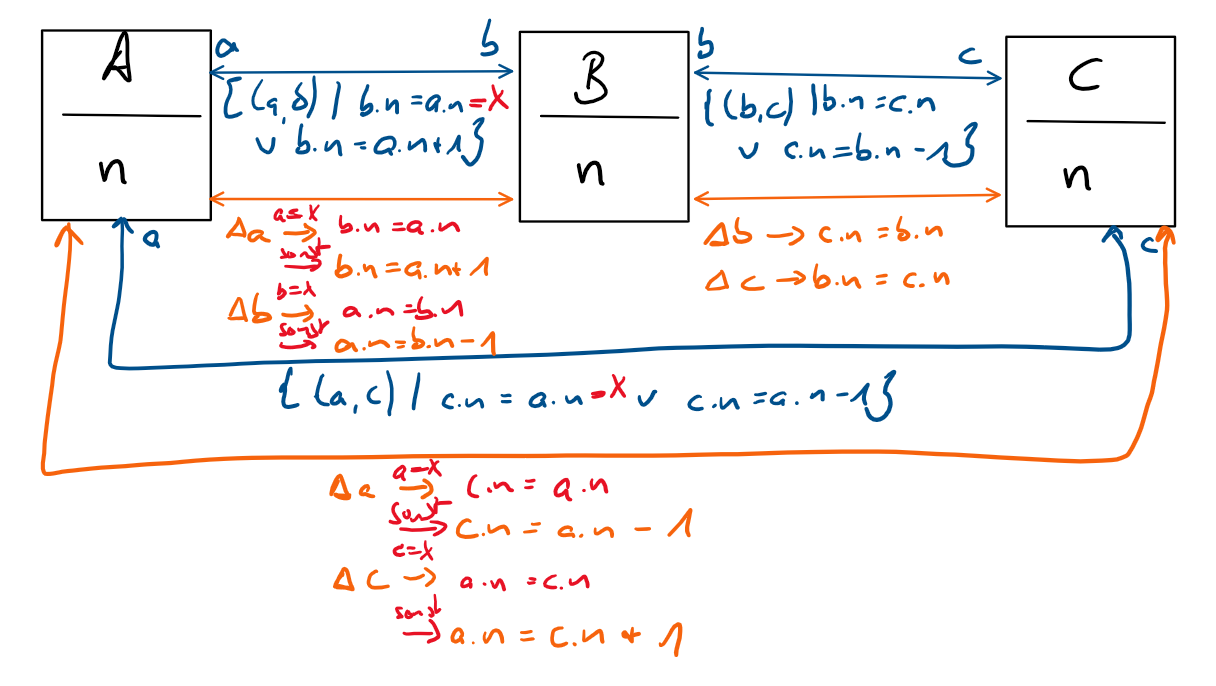
\includegraphics[width=\textwidth]{figures/correctness/orchestration/no_upper_bound_example_old.png}
%     \caption{Example for no upper bound}
%     \label{fig:formal:noupperboundexample}
% \end{figure}

% Depending on the value X, the transformations have to be executed X times to result in a consistent state. This value can be arbitrarily chosen, thus an arbitrary number of executions may be necessary to terminate in a consistent state.

% \todo{Moved from single execution section -> revise}
% \begin{theorem}[Orchestration with Unbounded Executions]
%     \label{theorem:unbounded_execution}
%     For any set of transformations $\transformationset{T}$, there can be models $\modeltuple{m}$ and changes $\changetuple{}$ to them for which each possible orchestration function $\orcfunction{\transformationset{T}}$ with whom $\appfunction{\orcfunction{\transformationset{T}}}(\modeltuple{m}, \changetuple{})$ is consistent, such that $\abs{\orcfunction{\transformationset{T}}(\modeltuple{m}, \changetuple{})} > \abs{\transformationset{T}}$.
% \end{theorem}
% \begin{proof}
%     We know from \autoref{lemma:minimal_executions} that $\transformationset{T}_{inc}$ requires at least $4$ executions of $\transformation{t}_{12}$ for the inputs defined in \autoref{lemma:minimal_executions} when selecting $x \geq 5$.
%     Thus, for any orchestration function, we know that $\abs{\orcfunction{\transformationset{T}}(\modeltuple{m}, \changetuple{})} > 4 > 3 = \abs{\transformationset{T}_{inc}}$.
%     This proves the theorem by example.
% \end{proof}


\subsection{Dynamic Detection of Alternation} % Divergence and alternation
\label{chap:orchestration:conservative:alternation}

\mnote{Orchestration requires abortion criterion}
The proposed algorithm, like any algorithm, is supposed to \emph{terminate} in a specific \emph{state} to be considered correct.
In our case, a correct state, as required by an application function it implements, is the return of consistent models or $\bot$, which the algorithm fulfills by construction.
In particular, the algorithm will never return models that are inconsistent, neither because it does not detect that they are inconsistent nor that it detects that they are inconsistent but still returns them.
From our previous findings regarding decidability, we know that we cannot expect the algorithm to realize an optimal application function.
Thus, we either need to implement \function{Orchestrate} such that it always returns $\bot$ after a finite number of executions to ensure termination, which results in returning $\bot$ although consistent models are expected, or we allow an arbitrary number of executions to improve the ability to find consistent results but accept that the algorithm may not terminate.

\mnote{Alternation is inifinte repeated passing of same state}
We have discussed that non-termination of the algorithm can occur because no consistent orchestration exists at all or because the algorithm is not able to find it.
A special case of non-termination is \emph{alternation}, which means that the same states are passed repeatedly. 
In case of transformation networks, alternation means that from some point in time the subsequent executions of the transformations in Line~\ref{algo:orchestration:application:line:stepcalculation} of \autoref{algo:orchestration:application} repeatedly produce the same sequence of results, i.e., of changes.
% Non-termination can, in general, manifest in terms of \emph{alternation} or \emph{divergence}, which means that either the same states are passed repeatedly or that an infinite sequence of different states is produced.
% In case of transformation networks, alternation means from some point in time the subsequent executions of the transformations in Line~\ref{algo:orchestration:application:line:stepcalculation} of \autoref{algo:orchestration:application} repeatedly produce the same sequence of results, i.e., of changes.
% Divergence means that from some point in time all results, i.e., changes, produced in Line~\ref{algo:orchestration:application:line:stepcalculation} differ.
In contrast to non-termination in general, the scenario of alternation can at least be avoided by construction.
% To this end, the history of change produced by the algorithm in Line~\ref{algo:orchestration:application:line:stepcalculation} has to be stored.
% It can either be used by the \function{Apply} function to detect alternation or by passing it to the \function{Orchestrate} function to influence the selection of transformations to avoid alternation.

\begin{definition}[Alternation of Apply Algorithmus]
    \label{def:applyalternation}
    Let there be a number $n$ of execution of the transformation execution loop in Lines~\autoref{algo:orchestration:application:line:startorchestrate}--\autoref{algo:orchestration:application:line:endorchestrate} of \autoref{algo:orchestration:application}, such that for all numbers of execution $> n$ there is a sequence of executed transformations and generated changes that occur at least two times subsequently at the end of the current states of $\applyalgexecuted$ and $\applyalggenerated$.
    Then we call the algorithm \emph{alternating}.
    If the algorithm does not terminate and is not alternating, we call it \emph{diverging}.
\end{definition}

\mnote{Orchestrate function can detect alternation}
The \function{Orchestrate} function receives the history of transformations and changes and is thus able to identify the situation that the same sequence of transformations was already executed and produced equal changes in each application.
This allows it to implement the function in a way that it does not return the same sequence of transformations when it was already passed and produced the same changes.
If a concrete realization of the \function{Orchestrate} function is not implemented in a way that it can react to the detection of alternation and produce a different sequence of transformations, it can at least return $\bot$ to ensure termination of \function{Apply}, because repeated execution of the same transformations will still returns the same changes. 

\mnote{Avoiding alternation improved possibility to find consistent orchestration}
Alternation produces orchestrations that can never yield consistent models, thus they are part of the problem space $P = {\transformationset{T}^{< \mathbb{N}}}$ of finding an orchestration for a given input $i$ of models and changes but can never be part of the solution space $S_{i} = \abs{\setted{\sequence{\transformation{t}} \in \transformationset{T}^{< \mathbb{N}} \mid \sequence{\transformation{t}} \mathtext{is consistent orchestration for} \tupled{\modeltuple{m}, \changetuple{\metamodeltuple{M}}}}}$ containing the consistent orchestrations.
Avoiding such alternations thus reduces the problem space without affecting the solution space and thus improves the possibility to find a consistent orchestration, as shown in the previous subsection.

%Divergence: If it passes the same changes again, then it either does not pass those changes again 

% Derive from the previous insights that whenever the algorithm does not terminate, we can have two situations: divergence and alternation.
% Prove that no other options for occurring situation exist!

% Problemraum:
% \begin{itemize}
%     \item Ziel ist, dass ein Netzwerk von Transformationen nach einer Änderung in einem konsistenten Zustand terminiert. D.h. Korrektheit stellt Anforderungen an \emph{Terminierung}, sowie den \emph{Zustand} bei Terminierung.
%     \item Folgende Abweichungen davon können auftreten:
%     \begin{enumerate}
%         \item Nicht-Terminierung: Das Netzwerk terminiert nicht. Das bedeutet im Prinzip, dass die Ausführungsfunktion (bzw. der Laufzeit-Algorithmus, der die Funktion dynamisch emuliert) nicht \emph{sound} ist. Soundness der Ausführungsfunktion setzt voraus, dass die berechnet Aufrufsequenz endlich ist. Wenn die Ausführung nicht terminiert, bedeutet das, dass entweder die gleichen Zustände mehrfach durchlaufen werden oder eine Sequenz unendlich vieler Zustände produziert wird. Denn wenn beides nicht der Fall ist, gibt es eine endliche Sequenz unterschiedlicher Zustände, d.h. Terminierung. Das bedeutet, dass es folgende zwei Möglichkeiten gibt:
%         \begin{itemize}
%             \item Alternierung: Die gleichen Zustände werden mehrfach durchlaufen.
%             \item Divergenz: Es werden unendlich viele Zustände produziert.
%         \end{itemize}
%         \item Inkonsistente Terminierung: Die Ausführungsfunktion bzw. der Algorithmus beendet die Ausführung, aber in einem inkonsistenten Zustand. Hier lassen sich ebenfalls wieder zwei Fälle unterscheiden.
%         \begin{itemize}
%             \item Unerkannte Inkonsistenz: Der Algorithmus terminiert und denkt, der Zielzustand wäre konsistent. Dies bedeutet aber direkt, dass nicht alle Konsistenzrelationen erfüllt sind, was, zumindest in der Theorie, einfach zu prüfen wäre (entweder durch Prüfung der Relationen oder durch Ausführung der hippokratischen Transformationen, die alle nichts tun dürften)
%             \item Erkannte Inkonsistenz: Der Algorithmus terminiert, wissend dass die Lösung nicht konsistent ist. Dies kann entweder sein, weil eine Transformation für zwei Modelle in einem inkonsistenten Zustand nicht mehr anwendbar ist, oder weil irgendein anderes Abbruchkriterium erreicht ist.
%         \end{itemize}
%     \end{enumerate}
% \end{itemize}

% Assume we have an algorithm that sequentially applies transformations.
% It stops as soon as a transformation cannot be applied or the models are consistent.
% Then we need to guarantee termination.
% We need to avoid that transformations can be applied indefinitely never leading to consistent models.

% Reasons for this situation are alternation and divergence.
% Prove that if we do not pass the same model state again (alternation) and if there is no indefinite number of model states (divergence), the algorithm terminates.
% Thus, if we ensure that any execution order of transformations does never lead to alternation and divergence, we know that the algorithm terminates!!

% \begin{itemize}
%     \item Zeigen, dass es Beispiele gibt, in denen es unabhängig von der Ausführungsreihenfolge immer zu einer Alternierung kommt
%     \item Zeigen, dass es Beispiele gibt, in denen es unabhängig von der Ausführungsreihenfolge immer zu einer Divergenz kommt.
%     \item Die Beispiele sollten zeigen, dass wir keine Einschränkungen an die Transformationen machen können, was das Problem aushebelt. D.h. egal welche Einschränkungen ich an die Transformationen definiere, es lassen sich immer Beispiele konstruieren, in denen es keine Ausführungsreihenfolge gibt, in denen sie terminieren.
%     \item Mathematisch zeigen, dass Alternierung und Divergenz die einzigen Probleme sind. D.h. wenn nicht der gleiche Zustand mehrmals durchlaufen wird (Alternierung) und es nicht unendlich viele Zustände gibt (Divergenz), dann ist die Folge endlich.
%     %\item Außerdem mathematisch die Abbildung von Transformationen auf Turing-Maschinen zeigen und damit ableiten, dass allgemeine Netzwerke erstmal nicht terminieren müssen (Abbildung auf Halteproblem)
% \end{itemize}

% To avoid these problems by construction, we discussed before that we need to achieve that P = S, such that the application function can execute transformations in an arbitrary order to achieve consistency.

% Another possibility would be to allow the problems and detect them dynamically and react to them.
% We will finally discuss that in the last section.

%In the following, we discuss whether and how we may restrict synchronizing transformations, such that an arbitrary execution order can avoid divergence and alternation, such that the algorithm terminates.


\subsection{Monotony for Avoiding Alternation}

\mnote{Non-alternation by construction instead of dynamic detection}
We have discussed %in \autoref{chap:orchestration:conservative:alternation}
that alternation, as a specific kind of non-termination scenario, can be avoided by construction of the orchestration function or at least can be detected by the \function{Apply} algorithm.
Instead of detecting alternation during orchestration, we may also restrict the transformation network such that no alternation can occur by construction.
We can achieve this by defining a notion of monotony for the transformations.

\mnote{Monotony notion from synchronizing transformations is not applicable}
For the construction of synchronizing bidirectional transformations by unidirectional consistency preservation rules in \autoref{chap:synchronization:bidirectional:transformations}, we have have defined the property of \emph{partial consistency improvement}, which is a monotony notion for the two unidirectional consistency preservation rules of a synchronizing bidirectional transformation, as each execution of them improved that property.
We can, however, not define monotony in a similar way for the whole transformation network because of two reasons.
First, the notion of partial consistency is not applicable for transformation networks, because each transformation needs to restore consistency between two models completely.
Second, since each transformation is developed independently from all others, we cannot apply the notion of partial consistent improvement to the other models by restricting how far a transformation may violate consistency to the other transformations.

We thus define a different notion of monotony for transformations as follows.
\begin{definition}[Monotone Synchronizing Transformation]
    \label{def:monotonetransformation}
    Let $\metamodeltuple{M} = \tupled{\metamodelsequence{M}{n}}$ be metamodels and let $\transformation{t}$ be a synchronizing transformation. We call $\transformation{t}$ monotone if it does not change elements that were already changed, i.e.
    \begin{align*}
        &
        \forall \modeltuple{m} = \tupled{\model{m}{1}, \dots, \model{m}{n}} \in \metamodeltuple{M}, \changetuple{\metamodeltuple{M}} = \tupled{\change{\metamodel{M}{1}}, \dots, \change{\metamodel{M}{n}}} \in \changeuniverse{\metamodeltuple{M}} : \\
        &
        \bigl(\exists \changetuple{\metamodeltuple{M}}' = \tupled{\change{\metamodel{M}{1}}', \dots, \change{\metamodel{M}{n}}'} \in \changeuniverse{\metamodeltuple{M}} : \generalizationfunction{\metamodeltuple{M},\transformation{t}}(\modeltuple{m}, \changetuple{\metamodeltuple{M}}) = \changetuple{\metamodeltuple{M}}' \\
        & \formulaskip
        \Rightarrow
        % WE CANNOT ASSUME TRANSFORAMTION TO BE STRONG MONTONE, BECAUSE IF TRANSFORMATION IS EXECTED FOR ALREADY CONSISTENT MODELS, IT CANNOT CHANGE ANYTHING
        % (\changetuple{\metamodeltuple{M}}'(\changetuple{\metamodeltuple{M}}(\modeltuple{m})) = \changetuple{\metamodeltuple{M}}(\modeltuple{m}) \Rightarrow \modeltuple{m} \consistenttomath \transformationset{T}) \\
        % & \formulaskip
        % \land 
        \forall i \in \setted{1, \dots, n} : 
        (\change{\metamodel{M}{i}}(\model{m}{i}) \setminus \model{m}{i} \subseteq \change{\metamodel{M}{i}}'(\change{\metamodel{M}{i}}(\model{m}{i})) \\
        & \formulaskip\formulaskip
        \land
        (\model{m}{i} \setminus \change{\metamodel{M}{i}}(\model{m}{i})) \cap \change{\metamodel{M}{i}}'(\change{\metamodel{M}{i}}(\model{m}{i})) = \emptyset)
        \bigr)
        %\change{\metamodeltuple{M}}(\modeltuple{m}) \subseteq \modeltuple{m} \cup \changetuple{\metamodeltuple{M}}'(\changetuple{\metamodeltuple{M}}(\model{m}{}))
        %\land
        %\modeltuple{m} \cup \changetuple{\metamodeltuple{M}}'(\changetuple{\metamodeltuple{M}}(\model{m}{})) \subseteq \changetuple{\metamodeltuple{M}}(\model{m}{})\big)
    \end{align*}
\end{definition}

\mnote{Montone transformations do not repeatedly change the same elements}
The definition is based on the idea that transformations are only supposed to append changes but not to revert previous changes.
This means that elements that were introduced by previous changes still need to be present after applying the transformation.
Additionally, elements that were removed are not allowed to be added by the transformation again.
Thus all elements of the originally changed models were either contained in the original models or are contained in the models yielded by the transformation application, which leads to the model relations in the definition.
Additionally, 

% \begin{definition}[Strongly Montone Synchronizing Transformation]
%     Let $\metamodeltuple{M}$ be metamodels and let $\transformation{t}$ be a monotone synchronizing transformation. We call $\transformation{t}$ strongly monotone if it does not perform any changes only when all models are already consistent does not change elements that were already changed, i.e.
% \end{definition}

\mnote{Orchestrations of monotone transforamtion yield squences of pairwise different model states}
Having only monotone transformations ensures that each orchestration, which does not apply a transformation to already consistent models, yields a sequence of pairwise different model states, if the transformations are sequentially applied.
\begin{lemma}[Montone Transformation Orchestration Prefixes]
    \label{lemma:monotonetransformationsnosamestates}
    Let $\transformationset{T}$ be a set of correct monotone synchronizing transformations for a tuple of metamodels $\metamodeltuple{M}$.
    Then for all models and changes, as well as any orchestration $\sequenced{\transformation{t}_{1}, \dots, \transformation{t}_{m}}  \; (\transformation{i} \in \transformationset{T})$ that does not contain a transformation when its models are already consistent, the prefixes of that orchestration only yield the same models if those prefixes are consistent orchestrations, i.e.
    \begin{align*}
        &
        \forall \modeltuple{m} \in \metamodeltupleinstanceset{M}, \changetuple{\metamodeltuple{M}} \in \changetuple{\metamodeltuple{M}} : \forall i, k \in \setted{1, \dots, m} : \\
        &
        \generalizationfunction{\metamodeltuple{M}, \transformation{t}_{i}} \concatfunction \dots \concatfunction \generalizationfunction{\metamodeltuple{M}, \transformation{t}_{1}}(\modeltuple{m}, \changetuple{\metamodeltuple{M}}) = \generalizationfunction{\metamodeltuple{M}, \transformation{t}_{k}} \concatfunction \dots \concatfunction \generalizationfunction{\metamodeltuple{M}, \transformation{t}_{1}}(\modeltuple{m}, \changetuple{\metamodeltuple{M}}) \\
        & \formulaskip 
        \Rightarrow
        \generalizationfunction{\metamodeltuple{M}, \transformation{t}_{k}} \concatfunction \dots \concatfunction \generalizationfunction{\metamodeltuple{M}, \transformation{t}_{1}}(\modeltuple{m}, \changetuple{\metamodeltuple{M}}) \consistenttomath \transformationset{T}
        \end{align*}
\end{lemma}
\begin{proof}
    Assume that there are two prefixes $\sequenced{\transformation{t}_{1}, \dots, \transformation{t}_{i}}$ and $\sequenced{\transformation{t}_{1}, \dots, \transformation{t}_{k}}$ of an orchestration, $i < k$ without loss of generality, such that they yield the same inconsistent models, i.e., $\generalizationfunction{\metamodeltuple{M}, \transformation{t}_{i}} \concatfunction \dots \concatfunction \generalizationfunction{\metamodeltuple{M}, \transformation{t}_{1}}(\modeltuple{m}, \changetuple{\metamodeltuple{M}}) = \generalizationfunction{\metamodeltuple{M}, \transformation{t}_{k}} \concatfunction \dots \concatfunction \generalizationfunction{\metamodeltuple{M}, \transformation{t}_{1}}(\modeltuple{m}, \changetuple{\metamodeltuple{M}})$ although $\generalizationfunction{\metamodeltuple{M}, \transformation{t}_{k}} \concatfunction \dots \concatfunction \generalizationfunction{\metamodeltuple{M}, \transformation{t}_{1}}(\modeltuple{m}, \changetuple{\metamodeltuple{M}})$ is not consistent to $\transformationset{T}$.
    We denote the change tuple delivered by any prefixes of length $l$ as $\changetuple{\metamodeltuple{M},l} = \tupled{\change{\metamodel{M}{1},l}, \dots, \change{\metamodel{M}{n}, l}}$ with $\tupled{\modeltuple{m}, \changetuple{\metamodeltuple{M},l}} = \generalizationfunction{\metamodeltuple{M}, \transformation{t}_{l}} \concatfunction \dots \concatfunction \generalizationfunction{\metamodeltuple{M}, \transformation{t}_{1}}(\modeltuple{m}, \changetuple{\metamodeltuple{M}})$.
    We know that the sequence of changes between the two prefixes does not perform any changes and thus acts like the identity function, i.e., $\generalizationfunction{\metamodeltuple{M}, \transformation{t}_{k}} \concatfunction \dots \concatfunction \generalizationfunction{\metamodeltuple{M}, \transformation{t}_{i+1}}(\modeltuple{m}, \changetuple{\metamodeltuple{M},i}) = \identitychange(\modeltuple{m}, \changetuple{\metamodeltuple{M},i})$
    and thus $\changetuple{\metamodeltuple{M},i}(\modeltuple{m}) = \changetuple{\metamodeltuple{M},k}(\modeltuple{m})$.
    We also know that all the transformations between the prefixes, i.e., all transformations $\transformation{t}_{l}$ for each $l$ with $i < l \leq k$, do not act like the identity function for their inputs, i.e., $\generalizationfunction{\metamodeltuple{M}, \transformation{t}_{l}}(\modeltuple{m}, \changetuple{\metamodeltuple{M},l-1}) \neq \identitychange(\modeltuple{m}, \changetuple{\metamodeltuple{M},l-1})$.
    Otherwise, the models affected by the transformation would either have been consistent before, which conflicts with the assumption that the orchestration does not contain a transformation when its models are already consistent, or they would not be consistent afterwards, which conflicts with the assumed correctness of the transformations.

    Thus, each transformation $\transformation{t}_{l} \; (i < l \leq k)$ performs modifications to the change tuple, i.e., adds or removed further elements.
    This especially applies to $\transformation{t}_{i+1}$.
    Let us assume that $\transformation{t}_{i+1}$ adds an element (analogous argumentation for the removal).
    %modifies the change tuple such that it adds or removes further elements.
    Then there is a model that contains the element after applying the change generated by the transformation, i.e., $\exists s \in \setted{1, \dots, n} : \exists \modelelement{e} : \modelelement{e} \in \change{\metamodel{M}{s},i+1}(\model{m}{s}) \setminus \change{\metamodel{M}{s},i}(\model{m}{s})$.
    Due to the transformations being monotone, we know that this element was not contained before, especially not in $\model{m}{s}$, as otherwise $\modelelement{e} \in \model{m}{s} \setminus \change{\metamodel{M}{s},i}(\model{m}{s})$ and thus $(\model{m}{s} \setminus \change{\metamodel{M}{s},i}(\model{m}{s})) \cap \change{\metamodel{M}{s},i+1}(\model{m}{s}) \neq \emptyset$, which conflicts the definition of monotone transformations for $\transformation{t}_{i+1}$.

    Since $\change{\metamodel{M}{s},k}(\model{m}{s}) = \change{\metamodel{M}{s},i}(\model{m}{s})$, we know that $\modelelement{e} \not\in \change{\metamodel{M}{s},k}(\model{m}{s})$.
    Thus, there must be a transformation $\transformation{t}_{l}$ with $i+1 < l \leq k$ which, in turn, removes this element, i.e., $\modelelement{e} \in \change{\metamodel{M}{s},l-1}(\model{m}{s}) \setminus \change{\metamodel{M}{s},l}(\model{m}{s})$.
    Then $\modelelement{e} \in \change{\metamodel{M}{s},l-1}(\model{m}{s}) \setminus \model{m}{s}$ and thus $\change{\metamodel{M}{s},l-1}(\model{m}{s}) \setminus \model{m}{s} \not\subseteq \change{\metamodel{M}{s},l}(\model{m}{s})$, which conflicts the definition of monotone transformations for $\transformation{t}_{l}$.

    In consequence, each transformation $\transformation{t}_{l} \; (i < l \leq k)$ can neither add nor remove an element, thus our assumption that two prefixes that yield the same inconsistent models does not hold, which proves the lemma.
\end{proof}

\mnote{Monotone transformation prevent alternation}
With that insight, it is easy to see that given only monotone transformation, no alternation can occur in our algorithm \autoref{algo:orchestration:application}.
\begin{theorem}[Monotone Transformations Prevent Alternation]
    Given a set of correct, monotone synchronizing transformations $\transformationset{T}$.
    Then \autoref{algo:orchestration:application} cannot contain an alternation according to \autoref{def:applyalternation}, as long as $\function{Orchestrate}$ does not return a transformation whose models are already consistent.
\end{theorem}
\begin{proof}
    According to \autoref{lemma:monotonetransformationsnosamestates}, monotone transformations ensure that in an orchestration that does not contains transformations that need to be applied to already consistent models the application of two prefixes never yields the same changes.
    In consequence, the sequence of $\applyalggenerated$ in the transformation application in 
    Lines~\autoref{algo:orchestration:application:line:startorchestrate}--\autoref{algo:orchestration:application:line:endorchestrate} of \autoref{algo:orchestration:application} can never contain the same two changes.
    This would, however, be necessary to fulfill \autoref{def:applyalternation} for alternation.
\end{proof}

\mnote{Guarantee by monotone transformations is stronger than non-alternation}
In fact, the guarantee of not producing the same state twice is even stronger than non-alternation, because alternation allows to pass the same state multiple times, as long as the same sequence of states is not passed repeatedly and infinitely.
It does, however, only make sense to pass the same state twice if the orchestration algorithm that selects the next transformation to execute is able to process that situation by trying different execution orders if an alternation occurs.
Thus, the less strict requirement for alternation is suited to make statements about the orchestration strategy but not about the individual transformations, as it is unlikely to find a property for a single transformation that gives a guarantee that depends on the execution order of transformations, like alternation does.

\mnote{Monotony cannot be generally assumed}
While monotone transformation give the guarantee of non-alternation, monotony according to \autoref{def:monotonetransformation} is not a property that we cannot assume to be fulfilled by all transformations.
Although is seems intuitive that a transformation should not remove elements that were added before and vice versa, this does also mean that, for example, an attribute value may only be changed once by the transformations.
This would, however, require the transformations to always make a choice for attributes that fits for all other transformations as well.
We have seen in different examples, such as the one depicted in \autoref{fig:orchestration:no_upper_bound} and \autoref{fig:orchestration:no_orchestration}, that it may be necessary to change elements multiple times, because the transformations select values with which the models only fulfill their own consistency relation but not those of the other transformations.
It may take several executions to find a value selection with which the models are consistent to all transformations.
We might say that the transformations need to \emph{negotiate} a consistent solution.

\mnote{Ensuring monotony as often as possible improves possibility of finding consistent orchestration}
Still, the given examples were rather artificial, so they cannot be seen as an indicator for monotony to be not practically achievable.
It may, at least in some cases, be possible to specify transformations that are monotone.
Even if only some of the transformations are monotone, or if only specific rules of them are monotone, it improves the chance that an orchestration strategy finds a consistent orchestration.
Having the knowledge about the benefits of monotony gives a transformation developer the ability to implement it as often as possible.

\mnote{Combining alternation avoidance and dynamic detection}
Finally, the possibility to avoid alternation by construction can be combined with the ability of an orchestration strategy to react to alternation.
We have discussed in \autoref{chap:orchestration:conservative:alternation} that an orchestration strategy can detect alternation and adapt its strategy of selecting the next transformation in that case.
In addition, if monotony is given at least for some transformations, the orchestration strategy needs to try less execution orders and thus improves the chance of finding a consistent orchestration.

% \begin{figure}
%     \centering
%     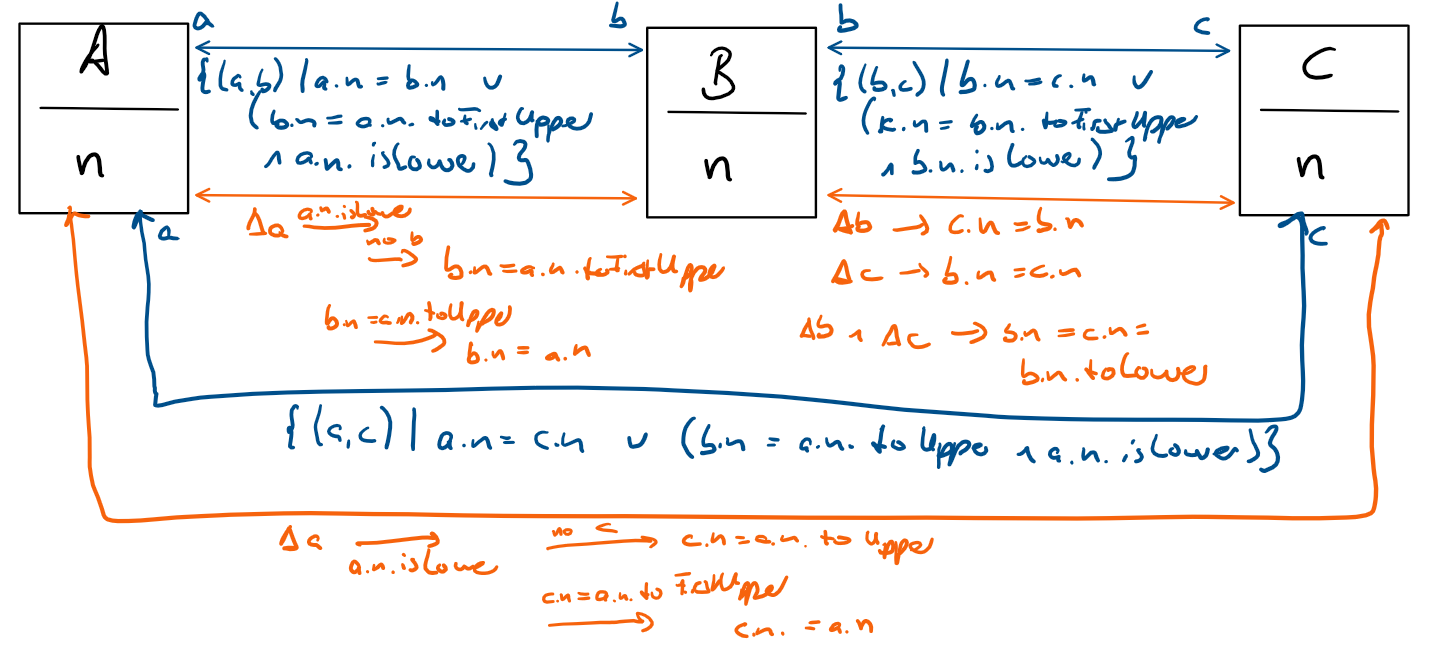
\includegraphics[width=\textwidth]{figures/correctness/orchestration/monotony_counterexample.png}
%     \caption{Counterexample for monotony}
%     \label{fig:formal:monotonycounterexample}
% \end{figure}

% \begin{itemize}
%     \item Muss eine Transformation mit jedem beliebigen Delta umgehen können müssen? Eine Einschränkung auf Monotonie würde dies verhindern. Bzw. wir müssten zeigen, dass es Konsistenzrelationen gibt, die unter der Anforderung an Monotonie nicht wiederhergestellt werden können. Bspw. fügt eine andere Transformation 3 Elemente hinzu, wo zwei mit dem anderen entsprechend der Konsistenzrelationen korrelieren und somit keine Witness-Struktur aufgebaut werden kann, die Konsistenz beweist. Das lässt sich durch Hinzufügen weiterer Elemente potentiell nicht auflösen (siehe Beispiele im SoSym-Paper).
%     \item Refer to synchronization chapter, where we introduced a monotony notion based on transformations being partial-consistency-improving. Here, in contrast, the CPRs cannot be aligned, such that we cannot, for example, expect one transformation not to lead to a reduction of consistency regarding consistency relations of other, previously executed transformations.
% \end{itemize}
% \begin{itemize}
%     \item Im Allgemeinen könnte eine Transformation beliebige dieser Deltasequenzen modifizieren. Wir verlangen jedoch, dass eine Transformation nur Deltas anhängt, also die Sequenzen länger werden
%     \item Genauer beschränken wir auch, welche Sequenzen eine Transformation sehen und ändern darf, genau gesagt darf sie die Sequenzen von zwei Modellen sehen und eine davon verlängern.
%     \item Hier kommt bereits der Unterschied zu bisherigen Transformationen, denn die sehen nur Deltas an einem Modell und erzeugen Deltas an dem anderen. Das ist bei uns schon gänzlich anders. Bidirektionale Transformationen unterstützen das im Übrigen auch nicht, sondern sind nur Spezifikationen, aus denen sich Wiederherstellungsroutinen für beide Richtungen ableiten lassen (siehe Stevens 2010)
% \end{itemize}

% \paragraph{Idea:} Require monotony to avoid alternation

% We would have to relax the definition of transformation to be monotone, because if a transformation is monotone, it may only append information, but this is not always possible, as can be seen in the following example. A monotone transformation must be able to return bottom if it cannot make further changes to restore consistency to the relation.

% \begin{definition}[Monotone Transformation]
%     Transformation gets models M and deltas D and produces new deltas D'. Taking the union of the original models M and the new models D'(M), then D(M) must be a subset of that, because other elements would have been added and removed afterwards or elements would have been changes once by D and again in a different way by D'.

%     Generally, monotony could also mean that only the same complete model state is not passed twice. \todo{Why dont we do that?}
% \end{definition}

% This would mean that each transformation only appends changes, i.e., if an element was added/removed, the transformation may not do the inverse. The same applies to attribute/reference changes: if an attribute/reference was already changes it may not be changed again.
% This way, it is by design impossible to pass through the same state again. Actually, if a monotone transformation returns bottom, the network has to terminate with a failure.
% However, this is hard restriction to transformations. It leads to the fact that in some networks that actually have a simple solution no solution is found at all. This can be easily seen at the example in \autoref{fig:formal:monotonycounterexample}. In the example adding "aa" to the left model, any execution order of the transformations leads to the situation that a previous change must be revoked to result in a consistent state. However, it is possible to derive a consistent state for that input change.

% \begin{figure}
%     \centering
%     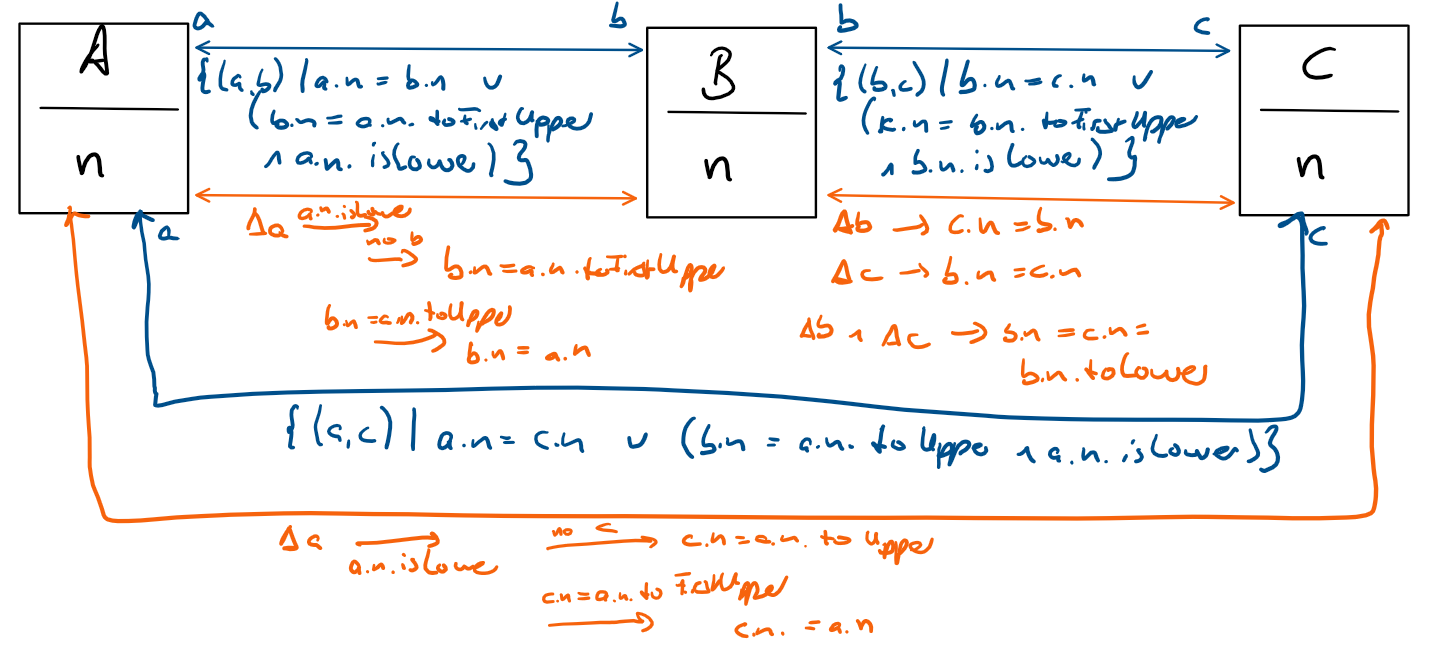
\includegraphics[width=\textwidth]{figures/correctness/orchestration/monotony_counterexample.png}
%     \caption{Counterexample for monotony}
%     \label{fig:formal:monotonycounterexample}
% \end{figure}

% One could now argue that there are binary relations in the example, which may never be fulfilled at all. We will later discuss how far relations that cannot be fulfilled should be restricted. However, in general, this is wanted behavior, because in general it may be necessary that transformations produce intermediate states that are not yet consistent with each other. Otherwise this would means that each transformation is always able to directly deliver a state that is consistent to all other relations, which is especially not possible, because other transformations may add further information to the models. More precisely, a relation may consider <a model consistent to all other models that contain any additional information not affected by the transformation. For example, a UML class model may be considered consistent to all Java models with any implementation of the specified methods, thus to an infinite number of models. Now saying that it should not be allowed that the transformation selects one with an empty implementation because that is not consistent to another relations induced by another transformation, such as the relationship to a component model, does not make any sense. Thus having those relation elements that may be considered locally consistent but will never occur in a globally consistent tuple of models does not make sense.
% In the example, we can see that such an inconsistent intermediate state is passed through and afterwards a consistent tuple of models is reached if not requiring monotony.
% In consequence, requiring monotony from transformations is a too strict requirement, because it is necessary to run through states that may be changed later on.

% \begin{theorem}
%     An application function for monotone transformations either returns a consistent model or produce a sequence of CPRs returning delta that return models of always growing size (i.e. it diverges).
% \end{theorem}

% \paragraph{Divergence cannot be avoided}

% There are rather equal network, one that terminates after a long time and one that never terminates. 
% Consider the example. The relations are defined in a way such that for any allocation for any of them a consistent tuple of models can be found. However, the transformations are not able to find it because they make "bad" choices from a set of choices that are conflicting. 
% This can be seen in the example that we have already given in \autoref{fig:correctness:no_execution_order}.

% Thus, systematically avoiding divergence is not possible. 

% \textbf{Central insight:} Alternation / Divergence cannot be avoided systematically (like in ordinary programming), if not restricting transformations in a way that may not be reasonable.


% \subsection{Unresolvability}

% Discuss why no execution order may exist although relations are compatible.
% If not even an order exists, the application function or the algorithm can, for sure, not find it.

% However, we found that we cannot always find an execution order if it exists and we were not able to find restrictions to transformations to ensure that it exists.
% We expect the same for the existence of an execution order at all.
% All restrictions we can make are likely to be too restrictive.
% The problem arises when there is an overlap of consistent models between some transformations, but they always decide for other elements that are not in the overlap of consistent models.
% It would, obviously, require the transformation to know about the others to ensure that this is not the case.
% This conflicts our assumption.

% Finally, it may be valid that for some changes no execution exists, because the change can not be processed on purpose \todo{Give example for that!}.
% Should this be the case if we assume compatibility?

% Although a more detailed investigation of the claim that we cannot define reasonable requirements to the transformations to ensure that they can always be ordered to restore consistency is a topic for further research, we did not investigate it in the scope of this thesis.
% Since we found it necessary to find a conservative algorithm that can deal with the case that no execution is found anyway, that algorithm covers the case that no execution order exists as well and thus is a solution for this problem as well.

% Beispiel:
% \begin{itemize}
%     \item Das ist im allgemeinen aber nicht Fall. Letztendlich trifft jede Transformation lokale Entscheidungen. Beispielsweise könnte jede einzelne Transformation gegeben eine beliebige Änderung immer dieselben Modelle (bzw. Änderungen die dazu führen) zurück liefern (im trivialsten Fall leere Modelle). Dann erfüllt jede Transformation ihre Korrektheitseigenschaft bzgl. ihrer Relation, aber das Netzwerk muss nicht korrekt sein, da bspw. T(A,B) und T(B,C) sich immer für verschiedene Instanzen von B entscheiden. Es gäbe somit nie eine konsistente Lösung für eine beliebige Ausführungsreihenfolge der Transformationen, auch wenn die Relationen das erlauben würden.
%     \item Beispiel mit Namen, wo eine Transformation immer den großen Namen zurück liefert, die andere immer den kleinen. T(A,B) bildet A auf gleiches B ab und beide auf kleine Schreibweise, obwohl beide erlaubt sind. Erzeuge A="a", dadurch B="a". T(B,C) bildet B auf C ab und beide auf große Schreibweise, obwohl beide erlaubt sind. Somit macht sie das zu B="A" und C="A". Nun wird T(A,B) wieder beide klein machen usw. Allerdings wäre eine insgesamt valide Lösung einfach alle groß oder alle klein zu machen, aber die Transformationen finden diesen Zustand nicht. 
% \end{itemize}

\section{A Conservative Application Algorithm}
\label{chap:orchestration:algorithm}

\mnote{Always terminating, correct algorithm}
We have argued why it is inevitable that any algorithm realizing an application function cannot be optimal and thus will not be able to find a consistent orchestration although it exists and, in that case, either return $\bot$ or not even terminate at all.
Apart from minor improvements, such as the avoidance or detection of alternations, to improve the probability to find a consistent orchestration, or general strategies like backtracking for trying different orchestrations, we did not find systematic ways to improve optimality of the application function.
Nevertheless, we want to find an algorithm that is at least correct and does always terminate, even if it does not implement a systematic way to improve optimality.
Thus it operates conservatively.

\mnote{Artificial execution bound drawback}
It is possible that \autoref{algo:orchestration:application} does not terminate, because it generates an infinitely long orchestration, thus never leaving the loop in Lines~\ref{algo:orchestration:application:line:startorchestrate}--\ref{algo:orchestration:application:line:endorchestrate}.
To ensure termination we need to introduce an upper bound for the number of executed transformations.
We have shown in \autoref{theorem:orchestration_fixed} that no natural upper bound exists, thus even the shortest consistent orchestration for specific inputs can be arbitrarily long. %(see example in \autoref{fig:orchestration:no_upper_bound}).
Any arbitrary bound can prevent the algorithm from finding consistent orchestrations.

\mnote{High number of executed transformation unwanted}
From an engineers perspective, we may, however, consider the behavior that an arbitrary high number of transformation executions is required to yield consistent models as unwanted.
Although the examples we have given are valid, they are rather artificial.
We claim that a transformation network that requires a rather high number of executions compared to the number of contained transformations to find consistent models does not operate as expected.
In particular, if such a high number of executions is required to find a consistent orchestration, it will be difficult to identify the reason for not finding a consistent execution in case the algorithm returns $\bot$.
Thus, we introduce an artificial upper bound for the number of transformation executions.
That bound will be well-defined, such that we can reasonably assume that no more executions are practically necessary.

\mnote{Design goals of orchestration}
In the following, we propose design goals for a conservative application algorithm and the so called \emph{provenance algorithm}, and finally prove its correctness and termination properties.
The algorithm was developed together with Joshua Gleitze in a scientific internship~\cite{gleitze2020orchestration}.

% FROM MODELS:
% Finally, one could question whether it is relevant if an execution strategy can be guaranteed to terminate. Execution strategies will be used to tell users whether changes they made can be incorporated into the other models automatically. In consequence, users should reliably and timely get a response. We might compare this situation to merging changes in version control systems. There, users also want a reliable and timely response on whether their changes could be incorporated automatically, or whether they need to resolve conflicts manually

% From an engineering perspective, unbounded numbers of executions is still unwanted behavior. We claim that a transformation network that takes thousands of executions of the same transformation to find a consistent state works not as expected and if running into a failure would expose severe problems to find the reasons for that failures.
% Thus, we propose to simply abort the execution after some time to be sure not to run in an endless loop.

% Finally, this problem is comparable to ordinary programming, because there the same situations regarding alternation and divergence can occur that result in non-termination of a program.
% As we all know, it is impossible to systematically avoid that, but just possible to carefully develop the program and apply best practices to avoid such situations.

% \textbf{Conclusion:} Apart from minor discussed improvements, we cannot systematically improve optimality / reduce conservativeness and also not dynamically terminate when divergence is detected. Especially, there is no guarantee wo when also alternation is detected. There can be an arbitrary high number of execution before alternation is detected.
% Thus, we propose an algorithm that terminates deterministically and returns $\bot$ also when it is not able to find a solution in a fixed number of steps, but improves the ability for the transformation developer or user to find out why in specific situation no solution can be found.

% \todo{Question whether having no upper bound is only a theoretical or also a practical problem. The given example is rather artificial, so we may stop in practice without excluding relevant cases}

\subsection{Design Goals}
\label{chap:orchestration:algorithm:goals}

\mnote{Degrees of freedom}
An adapted version of \autoref{algo:orchestration:application} that always terminates has two degrees of freedom.
First, the execution order of transformations needs to be determined by defining the function \function{Orchestrate}.
Second, an upper bound for the number of executions of transformations, thus the number of loop executions in Lines~\ref{algo:orchestration:application:line:startorchestrate}--\ref{algo:orchestration:application:line:endorchestrate}, needs to be defined.

\mnote{Importance of execution order}
We have discussed that improving optimality is not an achievable goal when determining the transformation execution order by the \function{Orchestrate} function.
Since we know that the algorithm will always produce false negatives, i.e., it will not find a consistent orchestration although it exists, it is important for a transformation developer or user to be able to identify the reasons for that in practice.
The algorithm can support them in this regard by delivering the final state of the models when the orchestration aborted.
The execution order that was chosen until that state was reached is of central importance for identifying the reasons for failing.
Consider that transformations are executed in an arbitrary order and then only some of the models of the final state are actually consistent.
Apart from investigating the complete sequence of executed transformations, there is no clue for the user to find the reasons for the algorithm to fail, thus about \emph{provenance} of the error.
We have introduced this goal as the \emph{comprehensibility} property in \autoref{chap:introduction:consistency:orchestration}.

\mnote{Incremental consistency restoration}
To improve identifying the reason whenever the algorithm fails, we propose the following principle for determining an orchestration:
\begin{quote}
    \enquote{Ensure consistency among the transformations that have already been executed before executing a transformation that has not been executed yet.}~\cite{gleitze2020orchestration}
\end{quote}
The principle requires that consistency is ensured incrementally for subsets of the transformations and thus the models.
As long as the models are not consistent to all already executed transformations, only those transformations instead of new ones may be executed until the models are consistent to all of them.
This ensures that consistency is preserved after each change in an incremental way, iteratively improving the number of models and transformations for which consistency is restored.

\mnote{Principle benefits}
This approach improves identifying provenance of a failure of the algorithm, because it restricts the potentially causal transformations to consider.
If the algorithm fails after executing a subset of the transformations $\transformationset{T}_\mathvariable{exec} \subseteq \transformationset{T}$,
then there is some transformation $\transformation{t} \in \transformationset{T}_\mathvariable{exec}$ that is the last of those transformation that was executed for its first time.
Thus, the algorithm found an orchestration of $\transformationset{T}_\mathvariable{exec} \setminus \transformation{t}$ such that the models were consistent to all those transformation, but it was not able to execute $\transformation{t}$ and the transformations in $\transformationset{T}_\mathvariable{exec}$ afterwards, such that the models become consistent to all these transformations.
This helps the transformation developer or user to understand and find the reason for failing in different ways.
First, he or she can ignore any transformation in $\transformationset{T} \setminus \transformationset{T}_\mathvariable{exec}$, as the algorithm already failed to preserve consistency according to the other transformations, which can significantly reduce the number of transformations to consider.
Second, the realization of $\transformation{t}$ is somehow conflicting with the other transformations in $\transformationset{T}_\mathvariable{exec}$. This does not necessarily mean that there is something wrong with $\transformation{t}$, but only that also considering this transformation either induces the situation that no consistent orchestration exists anymore or that it cannot be found.
Third, having a state of the models that is consistent to $\transformationset{T}_\mathvariable{exec} \setminus \transformation{t}$ can be used as a starting point to either identify the occurring problem or to manually restore consistency of the models.

\mnote{Principle not improving optimality}
If the algorithm operates according to the introduced principle and is not able to preserve consistency anymore after it considers an additional transformation $\transformation{t}$, the selected execution order provides the discussed benefits for identifying the reasons for failing.
There may, however, be another orchestration that is able to ensure consistency to $\transformationset{T}_\mathvariable{exec}$. Executing $\transformation{t}$ earlier or integrating further transformations in $\transformationset{T}$ before ensuring consistency to all transformations in $\transformationset{T}_\mathvariable{exec}$ can, of course, result in the algorithm finding a consistent orchestration.
This can reduce optimality of the realized orchestration function, but we claim the discussed benefits to outweigh that.

\mnote{Transformations reacting to others}
We have shown that there is no inherent upper bound for the necessary number of transformation executions.
Rather than specifying a concrete number, be it fixed or depending on the network size, we derive a reasonable artificial bound for the number of executions from a property that we assume reasonable for possible orchestrations of a transformation set.
The idea of that property is that each transformation should be allowed to react to the execution of each possible sequence of all other transformations.
It should, however, not be necessary that a transformation must be executed again after the other transformations reacted the execution of that transformation.
Thus, if a transformation was executed after applying the other transformations in any possible order, we expect the models to be consistent to that transformation.

\begin{definition}[Reactive Converging Transformations]
    \label{def:reactiveconverging}
    A set of synchronizing transformations $\transformationset{T}$ is \emph{reactive converging} with respect to models $\modeltuple{m}$ and changes $\changetuple{\metamodeltuple{M}}$ if any orchestration of any subset $\transformationset{T}_p \subseteq \transformationset{T}$ in which a transformation $\transformation{t} \in \transformationset{T}_P$ has been executed after a sequence of transformations in $\transformationset{T}_p$ that contains each permutation of those transformations as a (not necessarily continuous) subsequence yields models that are consistent to $\transformation{t}$.
\end{definition}

\mnote{Reactive converging transformations example}
The property does not require that the other transformations were executed in each order consecutively, but only that the orchestration contains each permutation of those transformations, but potentially with other transformations in between.
As an example, assume a set of transformations $\setted{\transformation{t}_{1}, \transformation{t}_{2}, \transformation{t}_{3}}$, which is reactive converging for some input of models and changes.
After executing them for these models and changes in the order $\sequenced{\transformation{t}_{1}, \transformation{t}_{2}, \transformation{t}_{3}, \transformation{t}_{1}, \transformation{t}_{2}, \transformation{t}_{3}}$, the models yielded by that orchestration may still be inconsistent to $\transformation{t}_{1}$, because it was not executed after the order of the transformations $\sequenced{\transformation{t}_{3}, \transformation{t}_{2}}$.
After executing $\transformation{t}_{1}$ once more, the orchestration must yield consistent models, because $\transformation{t}_{1}$ was executed after the two orders of the other transformations $\sequenced{\transformation{t}_{2}, \transformation{t}_{3}}$ and $\sequenced{\transformation{t}_{3}, \transformation{t}_{2}}$.
Likewise, $\transformation{t}_{2}$ was executed after $\sequenced{\transformation{t}_{1}, \transformation{t}_{3}}$ and $\sequenced{\transformation{t}_{3}, \transformation{t}_{1}}$, and $\transformation{t}_{3}$ was executed after $\sequenced{\transformation{t}_{1}, \transformation{t}_{2}}$ and $\sequenced{\transformation{t}_{2}, \transformation{t}_{1}}$.


\subsection{The Provenance Algorithm}

\begin{algorithm}
    \begin{algorithmic}[1]
\Procedure{\function{ProvenanceApply}}{$\transformationset{T}, \modeltuple{m}, \changetuple{\metamodeltuple{M}}$}
    \algindentskip
    \If{$\neg \function{CheckConsistency}(\transformationset{T}, \modeltuple{m})$}
        \State \Return{$\bot$} \label{algo:orchestration:provenance:line:bot_input}
    \EndIf
    \algblockskip

    \State $\changetuple{\metamodeltuple{M},\mathvariable{res}} \gets \function{Propagate}(\transformationset{T}, \modeltuple{m}, \changetuple{\metamodeltuple{M}})$
    \If{$\changetuple{\metamodeltuple{M},\mathvariable{res}} = \bot$}
        \State \Return{$\bot$} \label{algo:orchestration:provenance:line:bot_orchestration}
    \EndIf
    %\State $\modeltuple{m}_{res} \gets \changetuple{\metamodeltuple{M},\mathvariable{res}}(\modeltuple{m})$
    \algblockskip

    \State \Return{$\changetuple{\metamodeltuple{M},\mathvariable{res}}(\modeltuple{m})$} %$\modeltuple{m}_{res}$} 
    \label{algo:orchestration:provenance:line:return_result}
    \algindentskip
\EndProcedure
\vspace{0.5\baselineskip}

\Procedure{\function{Propagate}}{$\transformationset{T}, \modeltuple{m}, \changetuple{\metamodeltuple{M}}$}
    \algindentskip
    \State $\provalgexecuted \gets \emptyset$ \label{algo:orchestration:provenance:line:executed_init}
    %\State $\mathvariable{accumulatedChanges} \gets \changetuple{\metamodeltuple{M}}$         
    \algblockskip

    \For{$\provalgcandidate \in \transformationset{T} \setminus \provalgexecuted \mid \changetuple{\metamodeltuple{M}}.\mathvariable{affects}(\provalgcandidate)$} \label{algo:orchestration:provenance:line:loop_start}
        \algindentskip
        \State $\tupled{\modeltuple{m},\changetuple{\metamodeltuple{M},\mathvariable{candidate}}} \gets \generalizationfunction{\metamodeltuple{M}, \provalgcandidate}(\modeltuple{m}, \changetuple{\metamodeltuple{M}})$ \label{algo:orchestration:provenance:line:first_execution}
        \If{$\changetuple{\metamodeltuple{M},\mathvariable{candidate}} = \bot$}
            \State \Return{$\bot$} \label{algo:orchestration:provenance:line:bot_first_execution}
        \EndIf
        \algblockskip

        %\State $\transformationset{T}_{\mathvariable{subnetwork}} \gets \transformationset{T}.\mathvariable{edgeInducedSubgraph}(\transformationset{T}_\mathvariable{executed})$
        %\State $\changetuple{\metamodeltuple{M},\mathvariable{propagation}} \gets \function{Propagate}(\transformationset{T}_{\mathvariable{subnetwork}}, \modeltuple{m}, \changetuple{\metamodeltuple{M},\mathvariable{candidate}})$ \label{line:recursive-call}
        \State $\changetuple{\metamodeltuple{M},\mathvariable{propagation}} \gets \function{Propagate}(\provalgexecuted, \modeltuple{m}, \changetuple{\metamodeltuple{M},\mathvariable{candidate}})$ \label{algo:orchestration:provenance:line:recursive_call}
        \If{$\changetuple{\metamodeltuple{M},\mathvariable{propagation}} = \bot$}
            \State \Return{$\bot$} \label{algo:orchestration:provenance:line:bot_recursion}
        \EndIf
        \algblockskip

        \State $\tupled{\modeltuple{m},\changetuple{\metamodeltuple{M},\mathvariable{candidate}}} \gets \generalizationfunction{\metamodeltuple{M}, \provalgcandidate}(\modeltuple{m}, \changetuple{\metamodeltuple{M},\mathvariable{propagation}})$ \label{algo:orchestration:provenance:line:second_execution}
        \If{$\changetuple{\metamodeltuple{M},\mathvariable{candidate}} = \bot$}
            \State \Return{$\bot$} \label{algo:orchestration:provenance:line:bot_second_execution}
        \EndIf
        \algblockskip
        %\State $\changetuple{\metamodeltuple{M},\mathvariable{candidate}} \gets \mathvariable{candidate}.\mathvariable{execute}(\mathvariable{accumulatedChanges})$ \label{line:check-execution}
        %\State $\modeltuple{m}_{\mathvariable{propagation}} \gets \changetuple{\metamodeltuple{M},\mathvariable{candidate}}(\modeltuple{m})$ %\tupled{\change{\metamodel{M}{1},\mathvariable{propagation}}(\model{m}{1}), \dots, \change{\metamodel{M}{n},\mathvariable{propagation}}(\model{m}{n})}$
        %\algblockskip

        \If{$\neg \function{CheckConsistency}(\provalgexecuted, \changetuple{\metamodeltuple{M},\mathvariable{candidate}}(\modeltuple{m}))$} \label{algo:orchestration:provenance:line:bot_failcheck}
            \State \Return{$\bot$} \label{algo:orchestration:provenance:line:bot_nonreactiveconverging}
        \EndIf
        \algblockskip
        
        \State $\changetuple{\metamodeltuple{M}} \gets \changetuple{\metamodeltuple{M},\mathvariable{candidate}}$
        \State $\provalgexecuted \gets \provalgexecuted \cup \setted{\provalgcandidate}$ \label{algo:orchestration:provenance:line:executed_update}
        \algindentskip
    \EndFor
    \algblockskip

    \State \Return{$\changetuple{\metamodeltuple{M}}$}
    \algindentskip
\EndProcedure

\end{algorithmic}

	\caption[Provenance application algorithm]{The provenance algorithm. Adapted from \cite[Alg.~1]{gleitze2020orchestration}.}
	\label{algo:orchestration:provenance}
\end{algorithm}

\mnote{Recursive orchestration algorithm}
We propose an algorithm that realizes the discussed design goal with the function \function{ProvenanceApply} in \autoref{algo:orchestration:provenance}.
The algorithm is a derivation of the general algorithm implementing an application function depicted in \autoref{algo:orchestration:application}.
It first checks for consistency of the given models as a prerequisite for executing the transformations.
Then the algorithm calls the recursive function \function{Propagate}, which implements the orchestration of transformations and returns a change tuple that is yielded by the determined orchestration, which delivers consistent models if applied to the input models.
While this behavior is equal to the one in \autoref{algo:orchestration:application}, the orchestration itself is implemented differently in a recursive rather than an iterative manner, which implicitly ensures termination.

\mnote{Incremental consistency restoration principle}
The function \function{Propagate} implementing the orchestration in a recursive manner acts as follows.
It selects one of the transformations as a candidate to execute next.
This selection ensures that a transformation is selected whose models are affected by any already performed change, such that the transformation needs to perform changes.
Models are affected by a change if any of the two changes in $\change{\metamodeltuple{M}}$ for either of the models that are kept consistent by the selected transformation is not the identity function $\identitychange$.
It then applies the transformation using the generalization function $\generalizationfunction{}$.
If the selected transformation is not defined for the given models and changes, the function may return $\bot$, so that the complete algorithm terminates with $\bot$.
Afterwards, it recursively executes the function \function{Propagate} with the subnetwork given by the transformations that have already been executed and are stored in $\provalgexecuted$.
After that recursive execution it is checked whether the models yielded by the resulting changes are still consistent to the candidate transformation.
If this consistency check fails, the transformations do not fulfill the definition of being reactive converging according to \autoref{def:reactiveconverging}, as we prove later.
If the models are consistent to the transformation, the next candidate is picked.
In effect, the strategy realizes the defined principle in a recursive manner, because after executing a new transformations, the recursive execution ensures consistency to all already executed transformations by applying all already executed transformations again.

\begin{figure}
    \centering
    \usetikzlibrary{arrows.meta}

\newlength{\transformationdoublespacing}
\newlength{\transformationlinewidth}
\newlength{\transformationshorten}
\newlength{\transformationarrowwidth}
\newlength{\transformationarrowheight}
\newlength{\transformationbaselength}
\setlength{\transformationbaselength}{0.5pt}
\newcommand*{\settransformationscale}[1]{%
	\setlength{\transformationdoublespacing}{\dimexpr #1\transformationbaselength * 3 / 2\relax}%
	\setlength{\transformationlinewidth}{\dimexpr #1\transformationbaselength\relax}%
	\setlength{\transformationshorten}{\dimexpr #1\transformationbaselength * 5\relax}
	\setlength{\transformationarrowheight}{\dimexpr #1\transformationbaselength * 10\relax}%
	\setlength{\transformationarrowwidth}{\dimexpr \transformationarrowheight * 8 / 5\relax}%
	\tikzset{%
		halfsyncxarrow/.tip = {Latex[round,left,length=\the\transformationarrowheight,width=\the\transformationarrowwidth,angle'=45]},%
		halfsyncxarrow'/.tip = {Latex[round,right,length=\the\transformationarrowheight,width=\the\transformationarrowwidth,angle'=45]},%
		syncxarrow/.tip={Latex[round,length=\the\transformationarrowheight,width=\the\transformationarrowwidth,angle'=45]}%
	}%
}
\settransformationscale{1}
\tikzstyle{halfsyncx}=[
	-halfsyncxarrow,
	line width=\transformationlinewidth,
	line cap=round
]
\NewDocumentCommand{\halfsyncx}{O{} r()O{0pt} r()O{0pt} D<>{}}{%
	\path (#2) -- (#4) coordinate[at start](h1) coordinate[at end](h2);
	\draw [
		halfsyncx,
		shorten < = \transformationshorten+#3,shorten > = \transformationshorten+#5,#1
	]
	($(h1)!\transformationdoublespacing!90:(h2)$) -- ($(h2)!\transformationdoublespacing!-90:(h1)$)
	node[midway, above]{#6};
}
\NewDocumentCommand{\syncx}{O{} r()O{0pt} r()O{0pt} D<>{}}{
	\halfsyncx[#1] (#2)[#3] (#4)[#5] <#6>
	\halfsyncx[#1] (#4)[#5] (#2)[#3]
}


\newcommand{\modelradius}{0.1em}
\newcommand{\hmodeldistance}{1.07em}
\newcommand{\vmodeldistance}{0.9em}
\newcommand{\hnetworkdistance}{3.6*\hmodeldistance}
\newcommand{\vnetworkdistance}{4.15*\vmodeldistance}
\newcommand{\hborder}{0.4*\hmodeldistance}
\newcommand{\vborder}{0.4*\hmodeldistance}
\newcommand{\addnetworktopleft}[3]{
	\node[model,#2] (m#1left) {};
	\node[model, above right=\vmodeldistance and \hmodeldistance of m#1left.center, anchor=center] (m#1top) {};
	\syncx[unconsidered, #3] (m#1left) (m#1top)
}
\newcommand{\addnetworkmiddle}[2]{
	\node[model, below right=\vmodeldistance and \hmodeldistance of m#1left.center, anchor=center] (m#1bottom) {};
	\syncx[unconsidered, #2] (m#1top) (m#1bottom)
}
\newcommand{\addnetworktopright}[2]{
	\node[model, right=2*\hmodeldistance of m#1left.center, anchor=center] (m#1right) {};
	\syncx[unconsidered, #2] (m#1top) (m#1right)
}
\newcommand{\addnetworkbottomleft}[2]{
	\syncx[unconsidered, #2] (m#1left) (m#1bottom)
}
\newcommand{\addpseudobottom}[1]{
	\node[model, draw=none, fill=none, below right=\vmodeldistance and \hmodeldistance of m#1left.center, anchor=center] (m#1bottom) {};
}
\newcommand{\addpseudoright}[1]{
	\node[model, draw=none, fill=none, right=2*\hmodeldistance of m#1left.center, anchor=center] (m#1right) {};	
}

\newcommand{\drawnetworktopleft}[3]{
	\addnetworktopleft{#1}{#2}{#3}
	% Not necessary because no dependent networks, so save vertical space
	%\addpseudobottom{#1}
	%\addpseudoright{#1}
}
\newcommand{\drawnetworktopleftmiddle}[4]{
	\addnetworktopleft{#1}{#2}{#3}
	\addnetworkmiddle{#1}{#4}
	\addpseudoright{#1}
}
\newcommand{\drawnetworktop}[4]{
	\addnetworktopleft{#1}{#2}{#3}
	\addnetworktopright{#1}{#4}
	\addpseudobottom{#1}
}
\newcommand{\drawnetworktopmiddle}[5]{
	\addnetworktopleft{#1}{#2}{#3}
	\addnetworktopright{#1}{#4}
	\addnetworkmiddle{#1}{#5}
}
% #1: Number
% #2: Position of left model
% #3-#6: Properties of transformations (top left, top right, middle, bottom left)
\newcommand{\drawnetworkcomplete}[6]{
	\addnetworktopleft{#1}{#2}{#3}
	\addnetworktopright{#1}{#4}
	\addnetworkmiddle{#1}{#5}
	\addnetworkbottomleft{#1}{#6}
}
% #1: First network
% #2: Second network
\newcommand{\iteration}[2]{
	\draw[thick,-{>[scale=0.6]}] ($(#1right.east)+(0.5em,0)$) -- node[above,font=\scriptsize] {it} ($(#2left.west)+(-0.5em,0)$);
}
% #1: First network
% #2: Second network
\newcommand{\recursion}[2]{
	\draw[thick,-{>[scale=0.6]}] ($(#1bottom.south)+(0,-0.35em)$) -- node[right,font=\scriptsize] {rec} ($(#2top.north)+(0,0.35em)$);
}

\settransformationscale{0.75}

\begin{tikzpicture}[
	model/.style={draw, circle, fill=black, inner sep=\modelradius},
	executed/.style={color=blue!50},
	candidate/.style={color=red!50},
	unconsidered/.style={color=gray},
	every node/.append style={font=\scriptsize}
]
%\drawnetworkcomplete{1}{}{}{}{}{}

\node[fill=gray!10, above left=1*\vmodeldistance+1*\vborder and \hborder, anchor=north west, minimum width=2*\hmodeldistance+2*\hborder, minimum height=2*\vmodeldistance+2*\vborder] {};

\drawnetworkcomplete{2}{%right=\hnetworkdistance of m1left.center, anchor=center
}{candidate}{}{}{}

\node[fill=gray!10, above right=1*\vmodeldistance+1*\vborder and \hnetworkdistance-\hborder of m2left.center, anchor=north west, minimum width=2*\hmodeldistance+2*\hborder, minimum height=\vnetworkdistance+1*\vmodeldistance+2*\vborder] {};

\drawnetworkcomplete{3}{right=\hnetworkdistance of m2left.center, anchor=center}{executed}{candidate}{}{}
\iteration{m2}{m3}
\drawnetworktopleft{3-1}{below=\vnetworkdistance of m3left.center,anchor=center}{candidate}
\recursion{m3}{m3-1}

\node[fill=gray!10, above right=1*\vmodeldistance+1*\vborder and \hnetworkdistance-1*\hborder of m3left.center, anchor=north west, minimum width=\hnetworkdistance+2*\hmodeldistance+2*\hborder, minimum height=2*\vnetworkdistance+1*\vmodeldistance+2*\vborder] {};

\drawnetworkcomplete{4}{right=\hnetworkdistance of m3left.center, anchor=center}{executed}{executed}{candidate}{}
\iteration{m3}{m4}
\drawnetworktop{4-1}{below=\vnetworkdistance of m4left.center,anchor=center}{candidate}{}
\recursion{m4}{m4-1}
\node[fill=gray!20, above right=1*\vmodeldistance+1*\vborder and \hnetworkdistance-1*\hborder of m4-1left.center, anchor=north west, minimum width=2*\hmodeldistance+2*\hborder, minimum height=\vnetworkdistance+1*\vmodeldistance+2*\vborder] {};
\drawnetworktop{4-2}{right=\hnetworkdistance of m4-1left.center,anchor=center}{executed}{candidate}
\iteration{m4-1}{m4-2}
\drawnetworktopleft{4-2-1}{below=\vnetworkdistance of m4-2left.center,anchor=center}{candidate}
\recursion{[yshift=0.1*\vnetworkdistance]m4-2}{[yshift=0.1*\vnetworkdistance]m4-2-1}

\node[fill=gray!10, above right=1*\vmodeldistance+1*\vborder and 2*\hnetworkdistance-1*\hborder of m4left.center, anchor=north west, minimum width=3*\hnetworkdistance+2*\hmodeldistance+2*\hborder, minimum height=3*\vnetworkdistance+1*\vmodeldistance+2*\vborder] {};

\drawnetworkcomplete{5}{right=2*\hnetworkdistance of m4left.center, anchor=center}{executed}{executed}{executed}{candidate}
\iteration{[xshift=1*\hnetworkdistance]m4}{m5}
\drawnetworktopmiddle{5-1}{below=\vnetworkdistance of m5left.center,anchor=center}{candidate}{}{}
\recursion{m5}{m5-1}
\node[fill=gray!20, above right=1*\vmodeldistance+1*\vborder and \hnetworkdistance-1*\hborder of m5-1left.center, anchor=north west, minimum width=2*\hmodeldistance+2*\hborder, minimum height=\vnetworkdistance+1*\vmodeldistance+2*\vborder] {};
\drawnetworktopmiddle{5-2}{right=\hnetworkdistance of m5-1left.center,anchor=center}{executed}{candidate}{}
\iteration{m5-1}{m5-2}
\drawnetworktopleft{5-2-1}{below=\vnetworkdistance of m5-2left.center,anchor=center}{candidate}
\recursion{m5-2}{m5-2-1}
\node[fill=gray!20, above right=1*\vmodeldistance+1*\vborder and \hnetworkdistance-1*\hborder of m5-2left.center, anchor=north west, minimum width=\hnetworkdistance+2*\hmodeldistance+2*\hborder, minimum height=2*\vnetworkdistance+1*\vmodeldistance+2*\vborder] {};
\drawnetworktopmiddle{5-3}{right=\hnetworkdistance of m5-2left.center,anchor=center}{executed}{executed}{candidate}
\iteration{m5-2}{m5-3}
\drawnetworktopleftmiddle{5-3-1}{below=\vnetworkdistance of m5-3left.center,anchor=center}{candidate}{}
\recursion{m5-3}{m5-3-1}
\node[fill=gray!30, above right=1*\vmodeldistance+1*\vborder and \hnetworkdistance-1*\hborder of m5-3-1left.center, anchor=north west, minimum width=2*\hmodeldistance+2*\hborder, minimum height=1*\vnetworkdistance+1*\vmodeldistance+2*\vborder] {};
\drawnetworktopleftmiddle{5-3-2}{right=\hnetworkdistance of m5-3-1left.center,anchor=center}{executed}{candidate}
\iteration{m5-3-1}{m5-3-2}
\drawnetworktopleft{5-3-2-1}{below=\vnetworkdistance of m5-3-2left.center,anchor=center}{candidate}
\recursion{m5-3-2}{m5-3-2-1}

% Legend
\newcommand{\vdistancelegend}{1*\vmodeldistance}
%\coordinate (legend_left_column) at ([yshift=-2.53*\vnetworkdistance]m2left.center);
\coordinate (legend_left_column) at ([yshift=-1.6*\vnetworkdistance,xshift=0.2em]m2left.center);

\node[draw, legendbg, minimum height=6.9*\vdistancelegend, minimum width=7.2em, above right=1.1*\vdistancelegend and -0.75em of legend_left_column, anchor=north west] {};

\syncx[] (legend_left_column) ([xshift=1*\hmodeldistance]legend_left_column)
\node[right=1.3*\hmodeldistance of legend_left_column,anchor=west] {$\transformationset{T}$};
\syncx[candidate] ([yshift=-\vdistancelegend]legend_left_column) ([xshift=1*\hmodeldistance,yshift=-\vdistancelegend]legend_left_column)
\node[below right=\vdistancelegend and 1.3*\hmodeldistance of legend_left_column,anchor=west] {$\provalgcandidate$};
\syncx[executed] ([yshift=-2*\vdistancelegend]legend_left_column) ([xshift=1*\hmodeldistance,yshift=-2*\vdistancelegend]legend_left_column)
\node[below right=2*\vdistancelegend and 1.3*\hmodeldistance of legend_left_column,anchor=west] {$\provalgexecuted$};

\coordinate (legend_right_column) at ([yshift=-3.8*\vdistancelegend]legend_left_column); %([xshift=7em]legend_left_column);

\coordinate (legenditerationright) at ([xshift=-0.3*\hmodeldistance+\modelradius]legend_right_column);
\coordinate (legenditerationleft) at ([xshift=-0.3*\hmodeldistance-2*\hmodeldistance-\modelradius+\hnetworkdistance]legend_right_column);
\iteration{legenditeration}{legenditeration}
\node[right=1.3*\hmodeldistance of legend_right_column, anchor=west] (legenditerationtext) {iteration step};

\coordinate (legendrecursionbottom) at ([yshift=-\vdistancelegend+0.5*\vnetworkdistance-\vmodeldistance-\modelradius]legend_right_column);
\coordinate (legendrecursiontop) at ([yshift=-\vdistancelegend-0.5*\vnetworkdistance+\vmodeldistance+\modelradius]legend_right_column);
\recursion{legendrecursion}{legendrecursion}
\node[below=\vdistancelegend of legenditerationtext.west, anchor=west] {recursion step};

\end{tikzpicture}%
    \caption[Exemplary execution of the provenance algorithm]{%
    Exemplary execution of the provenance algorithm for a change in the topmost model. 
    The transformations present to the current execution of \function{Propagate}, as well as the executed and candidate transformations $\provalgexecuted$ and $\provalgcandidate$ are depicted for each iteration (horizontal) and recursion step (vertical). Taken from \cite[Fig.4]{gleitze2020orchestration}.
}
    \label{fig:orchestration:provenance_example}
\end{figure}

\mnote{Exemplary algorithm execution}
\autoref{fig:orchestration:provenance_example} depicts an exemplary execution of the \function{ProvenanceApply} algorithm for a set of four transformations between four metamodels.
We assume that the algorithm receives four initially consistent models and a change to the topmost one.
The example shows that in each recursion step only the subnetwork of the already executed transformations in $\provalgexecuted$ is considered.
Thus, the set of transformations becomes smaller in each recursive call of \function{ProvenanceApply}.


\subsection{Correctness, Termination and Goal Fulfillment}

\mnote{Properties fulfillment}
The provenance algorithm was intended to implement a correct application function and to always terminate.
Additionally, it is supposed to deliver consistent models whenever the given transformations fulfill \autoref{def:reactiveconverging} for being reactive converging.
In the following, we prove that the algorithm actually fulfills these properties.

\mnote{Termination and correctness}
First, it is easy to see that the algorithm always terminates and always either returns consistent models yielded by an orchestration of the given transformations or $\bot$, which realizes a correct application function according to \autoref{def:applicationfunction} and \autoref{def:applicationfunctioncorrectness}.

\begin{theorem}[Provenance Algorithm Termination]
    \autoref{algo:orchestration:provenance} terminates for every possible input.
\end{theorem}
\begin{proof}
    The algorithm terminates if \function{CheckConsistency}, $\generalizationfunction{}$ and \function{Propagate} terminate.
    We assume termination for the external function \function{CheckConsistency}, because it only validates consistency of the given models.
    \function{Propagate} contains a loop with a recursive call and the external calls of \function{CheckConsistency} as well as $\generalizationfunction{}$.
    Since \function{CheckConsistency} and $\generalizationfunction{}$ terminate, it may only be non-terminating because of the loop in Line~\ref{algo:orchestration:provenance:line:loop_start} and the recursive call in Line~\ref{algo:orchestration:provenance:line:recursive_call}.
    The number of loop executions is limited by the number of given transformations, i.e., $\abs{\transformationset{T}}$, as each iteration selects another transformation and adds it to $\provalgexecuted$, thus after selecting each transformation once, all transformations are in $\provalgexecuted$ and thus the loop condition is not fulfilled.
    The recursive call receives a set of transformations that is at least one element smaller than the set of transformations given to the calling method, because if $\provalgexecuted = \transformationset{T}$ the loop precondition is not fulfilled. If the given set of transformations is empty, the loop is not entered and thus no recursive call is performed. Thus, the recursion depth never exceeds $\abs{\transformationset{T}}$.
\end{proof}

\begin{theorem}[Provenance Algorithm Correctness] \label{theorem:provenance_correctness}
    \autoref{algo:orchestration:provenance} realizes a correct application function. % according to \autoref{def:applicationfunctioncorrectness}.
\end{theorem}
\begin{proof}
    The algorithm receives models and changes to them and it returns models being instances of the same metamodels, thus it fulfills the signature of an application function.
    Additionally, if it returns models, they are the result of a consecutive application of transformations in $\transformationset{T}$, as \function{Propagate} calculates the changes that are applied to the input models to calculate the result by a repeated application of the generalization function $\generalizationfunction{}$ to transformations in $\transformationset{T}$.
    Thus, \function{Propagate} implicitly implements an orchestration function according to \autoref{def:orchestrationfunction} and applies the transformations in the determined order to calculate the result delivered by \function{ProvenanceApply}.
    Thus, \function{ProvenanceApply} fulfills \autoref{def:applicationfunction} for an application function.

    Let us assume that \autoref{algo:orchestration:provenance} does not realize a correct application function.
    \function{ProvenanceApply} may return $\bot$ in \autoref{algo:orchestration:provenance:line:bot_input} or \autoref{algo:orchestration:provenance:line:bot_orchestration}, or it may return models in \autoref{algo:orchestration:provenance:line:return_result}.
    Correctness requires the function to either return $\bot$ or consistent models, which may only be violated by \function{ProvenanceApply} returning inconsistent models.
    This means that for some input models and changes, \function{ProvenanceApply} returns models $\modeltuple{m}_\mathvariable{res}$, such that there is a transformation $\transformation{t} \in \transformationset{T}$ to which $\modeltuple{m}_\mathvariable{res}$, or more specifically two models $\model{m}{i}$ and $\model{m}{k}$, 
    whose metamodels are related by $\transformation{t}$, are not consistent.
    We distinguish three cases:
    \begin{longenumerate}
        \item $\transformation{t}$ was never executed by \function{Propagate}. This means that the changes $\change{\metamodel{M}{i}}$ and $\change{\metamodel{M}{k}}$ in $\change{\metamodeltuple{M}}$ of the two models that are kept consistent by $\transformation{t}$ were always empty, i.e., $\identitychange$, because otherwise $\transformation{t}$ would have been selected in the loop header. Since the initial models $\model{m}{i}$ and $\model{m}{k}$ were consistent to $\transformation{t}$, the returned models are still consistent, because only the identity function is applied to them.
        \item $\transformation{t}$ was executed and no other transformation that involves $\model{m}{i}$ or $\model{m}{k}$ was executed afterwards. Then the returned models are consistent by definition of correctness for $\transformation{t}$.
        \item $\transformation{t}$ was executed and another transformation $\transformation{t}' \in \transformationset{T}$ that involves $\model{m}{i}$ or $\model{m}{k}$ was executed afterwards.
        Since $\transformation{t}'$ was executed after $\transformation{t}$, $\transformation{t}$ was in $\provalgexecuted$ when $\transformation{t}'$ was the candidate transformation $\provalgcandidate$.
        Thus, $\transformation{t}$ is executed in the recursion after the first execution of $\transformation{t}'$, thus the result is consistent to $\transformation{t}$ and because of the check in Line~\ref{algo:orchestration:provenance:line:bot_failcheck} after returning from the recursion also to $\transformation{t}'$. Thus, the returned models are consistent to both $\transformation{t}$ and $\transformation{t}'$.
    \end{longenumerate}
    The third case can be applied inductively if a transformation is followed by multiple transformations that involve the same models. Thus, all cases lead to a contradiction.
\end{proof}

\mnote{Algorithm complexity}
In addition to these essential properties, we can also derive the upper bound for the number of transformation executions by the algorithm.

\begin{theorem}[Provenance Algorithm Complexity]
    \autoref{algo:orchestration:provenance} executes transformations at most $\mathcal{O}(2^{\abs{\transformationset{T}}})$ times.
\end{theorem}
\begin{proof}
	Let $T(m)$ denote the number of transformation executions the algorithm invokes for a set of transformations $\transformationset{T}$ with $m = \abs{\transformationset{T}}$.
	The set $\provalgexecuted$ is initialized to be empty (Line~\ref{algo:orchestration:provenance:line:executed_init}) and grows by one transformation every iteration of the loop (Line~\ref{algo:orchestration:provenance:line:executed_update}).
    It follows that the recursive call in Line~\ref{algo:orchestration:provenance:line:recursive_call} receives a set of transformations that contains one more transformation in each iteration.
    Thus, given $m$ transformations, \function{Propagate} executes each of them in the loop and then makes recursive calls for $0$ to $m-1$ transformations:
    \begin{align*}
        &
    T(m)	=m+\sum_{i=0}^{m-1}T(i)
    	=2+2\,T(m-1)
        =2*(2^{m}-1) \in \mathcal{O}(2^m) \\
        &
    T(0)	=0 \qedhere
	\end{align*}
\end{proof}

\mnote{Design principle fulfillment}
Finally, the algorithm shall implement the principle defined in \autoref{chap:orchestration:algorithm:goals} to ensure consistency among the transformations that have already been executed before executing a transformation that has not been executed yet.

\begin{theorem}[Provenance Algorithm Design Principle]
    \autoref{algo:orchestration:provenance} ensures consistency among the transformations that have already been executed before executing a transformation that has not been executed yet.
\end{theorem}
\begin{proof}
	After the recursive call in Line~\ref{algo:orchestration:provenance:line:recursive_call}, the current model tuple $\modeltuple{m}_{\mathvariable{propagation}}$ is consistent to all executed transformations in $\provalgexecuted$ according to \autoref{theorem:provenance_correctness}. % and
%	\Cref{thm:strategy-correct} applies for every recursive execution of the strategy. 
	%no changes to models involved  to an executed transformations are allowed.% after the recursive call in \cref{line:recursive-call}.
%	Hence,
	% \executed is either empty or 
%	the current model assignment is consistent with all transformations in \executed whenever the algorithm executes a new transformation in \cref{line:first-execution}.
\end{proof}	

\mnote{Algorithm optimality}
We have given \autoref{def:reactiveconverging} for the property of a transformation set to be reactive converging.
This property defines that we do not want transformations to be required to react to changes they performed themselves if all other transformations have been executed afterwards, as we assume this to be a reasonable property that induces an upper bound for the number of transformation executions.
We have used that property as a design goal for the proposed algorithm and can now show that the algorithm always returns consistent models when the transformations fulfill that property, which means that the algorithm implements an optimal application function.

\begin{theorem}[Provenance Algorithm Optimality]
    If the transformation set $\transformationset{T}$ passed to \autoref{algo:orchestration:provenance} is reactive converging according to \autoref{def:reactiveconverging} and if the consistency preservation rules of all transformations in $\transformationset{T}$ are total functions, the algorithm implements an optimal application function.
\end{theorem}
\begin{proof}
    We show that the algorithm does not return $\bot$ when the input models are consistent, thus an orchestration is always found.
    This is even stronger than optimality, because it means that for every input with consistent models a consistent orchestration exists.

    Since optimality allows the algorithm to return $\bot$ when the input models are inconsistent, returning $\bot$ in \autoref{algo:orchestration:provenance:line:bot_input} is valid.
    The algorithm returns $\bot$ in \autoref{algo:orchestration:provenance:line:bot_orchestration} if \function{Propagate} returns $\bot$, thus we show that \function{Propagate} does not return $\bot$.
    \function{Propagate} returns $\bot$ in \autoref{algo:orchestration:provenance:line:bot_application} if the application of a selected transformation in \autoref{algo:orchestration:provenance:line:first_execution} returns $\bot$, which cannot occur because transformation are total by assumption.
    \function{Propagate} returns $\bot$ in \autoref{algo:orchestration:provenance:line:bot_recursion} if a recursive call returns $\bot$. If the loop in that recursive call is executed, the arguments for not returning $\bot$ apply recursively. If the loop is not executed in the recursion, the input changes are returned, thus not yielding $\bot$.
    
    Finally, \function{Propagate} returns $\bot$ in \autoref{algo:orchestration:provenance:line:bot_nonreactiveconverging} if the models yielded by the recursive call are not consistent with the transformation that is the candidate $\provalgcandidate$ in that loop iteration.
    Since the transformation set is reactive converging, this can only be the case if not all permutations of the transformations currently in $\provalgexecuted$ have been executed yet.
    We show that all transformations in $\provalgexecuted$ have been executed in every order by induction.
    In the first iteration of the loop only the candidate of that iteration is executed and $\provalgexecuted$ is empty, thus the statement is trivially true.
    Let us assume that in a loop iteration with $\abs{\provalgexecuted} = i-1$ all permutations of transformations in $\provalgexecuted$ have been executed in Line~\ref{algo:orchestration:provenance:line:bot_nonreactiveconverging}, but that in the following loop iteration with $\abs{\provalgexecuted} = i$ this is not true.
    This means that there is an order $\sequenced{\transformation{t}_{1}, \dots, \transformation{t}_{i}}$ of the transformations in $\provalgexecuted$, in which they have not been executed yet.
    Let $\transformation{t}$ be the candidate $\provalgcandidate$ of the last iteration with $\abs{\provalgexecuted} = i-1$. Let $k$ be the index of $\transformation{t}$ in that sequence, i.e., $\transformation{t} = \transformation{t}_{k}$. Then per induction assumption the sequence $\sequenced{\transformation{t}_{1}, \dots, \transformation{t}_{k}}$ has been executed in one of the previous iterations of the loop. 
    Afterwards $\transformation{t}$ was executed in Line~\ref{algo:orchestration:provenance:line:first_execution}.
    Additionally, the sequence $\sequenced{\transformation{t}_{k+1}, \dots, \transformation{t}_{i}}$ has been executed in the recursive call in Line~\ref{algo:orchestration:provenance:line:recursive_call} by induction assumption.
    Hence, the transformations have been executed in the order $\sequenced{\transformation{t}_{1}, \dots, \transformation{t}_{i}}$, which is a contradiction to our assumption.

    In consequence, \function{Propagate} and thus \function{ProvenanceApply} does never return $\bot$, except for inconsistent input models. Since we have already proven that the algorithm terminates always and implements a correct application function, it implements an optimal application function.
\end{proof}

\mnote{Optimality assumptions fulfillment}
Optimality can, however, only be guaranteed under specific conditions.
Apart from the necessary to be reactive converging, the transformations need to be able to handle every input, thus every combination of models and changes, as otherwise selecting a transformation may lead to \function{Propagate} returning $\bot$, because the transformation cannot be applied.
In practice, this assumption will usually not be fulfilled.
Nevertheless, it is theoretically possible to define such transformations and at least it leads to well-defined conditions for when we can assume the algorithm to realize an optimal orchestration function.

\mnote{Orchestration problem non-existence}
Although this means that under such specific conditions the algorithm is able to decide the orchestration problem, the problem is actually trivially solved in that case, because for every input there is a consistent orchestration, thus the problem is actually non-existent under these assumptions.

\mnote{Well-defined requirements}
Finally, it is an open question how far we can assume sets of transformations to be reactive converging in practice.
We have, however, not introduced this as a property that should be fulfilled by transformations, as it is obviously hard to ensure or even analyze that property.
In fact, it is only supposed to be a well-defined property that allows us to define a reasonable upper bound for the execution of transformations and thus to allow us to define an algorithm that always terminates without using a completely arbitrary upper bound for determining when to terminate.


\subsection{Provenance Identification Improvement}

\mnote{Information about failure state}
We have motivated the provenance algorithm with the idea to improve the ability of a transformation developer or user to find the reason for the algorithm not to yield consistent models for certain inputs.
The proposed \autoref{algo:orchestration:provenance} only returns $\bot$ in those situations and thus does not directly support that process.
The necessary information for improving the identification of provenance for the failure is, however, present in the algorithm and can be easily retrieved.

\mnote{Reasons for algorithm failing}
The algorithm may fail, because it is, at some point, not able to execute a candidate transformation (Line~\ref{algo:orchestration:provenance:line:bot_application}), or because after executing a new transformation consistency to the previously executed transformations cannot be achieved without letting one of the transformations react to the reaction of all other transformations to its own changes (Line~\ref{algo:orchestration:provenance:line:bot_failcheck}), which we defined as the property of reactive convergence.
In that case, we at least know that after the previous loop iteration consistency to all transformations that have been executed so far could be achieved.

\mnote{Relevant failure state information}
Whenever the \function{Propagate} function fails and returns $\bot$, we know that for the current transformations in $\provalgexecuted$ an orchestration exists that yields the current changes in $\changetuple{\metamodeltuple{M}}$, %= \tupled{\change{\metamodel{M}{1}}, \dots, \change{\metamodel{M}{n}}}$
for which we know that applied to the original models, the result $\changetuple{\metamodeltuple{M}}(\modeltuple{m})$ %\tupled{\change{\metamodel{M}{1}}(\model{m}{1}), \dots, \change{\metamodel{M}{n}}(\model{m}{n})}$
is at least consistent to $\provalgexecuted$.
We also know that the algorithm was not able to ensure consistency to the current candidate transformation $\provalgcandidate$.
This is exactly the information for which we already discussed in \autoref{chap:orchestration:algorithm:goals} the benefits with respect to the underlying design principle of recursively ensuring consistency for subsets of the transformations for the ability to identify the reasons for not finding a consistent orchestration.
Thus, implementing the algorithm such that it also delivers $\provalgcandidate$, $\provalgexecuted$ and the current changes $\changetuple{\metamodeltuple{M}}$ reduces the necessary model states and transformations to consider for a transformation user or developer to identify why no consistent orchestration was found.

%Unfortunately, the algorithm does help in finding whether no orchestration exists at all or whether only the algorithm was not able to find it.
%Maybe map that to inapplicability of transformations to non-existence vs. fail after recursive application to non-finding

\mnote{Improving locality}
The algorithm and the ability to identify reasons for the algorithm to fail may be further improved by determining a reasonable order for the execution of transformations in the loop of the \function{Propagate} function.
The loop at least ensures that no transformations are executed that are not yet affected by any change and thus would not produce changes.
It can, however, also be reasonable to first select transformations for which both models have already been modified before selecting transformations for which only one model has been modified.
This can further improve locality of the changes made until the algorithm fails, because less models may have been modified until the algorithm fails.
We also discuss these benefits as results of the evaluation in \autoref{chap:correctness_evaluation:orchestration}.

%\todo{Discuss that is may make sense to first use transformations between already involved models rather than passing through the complete network.}



\section{Summary}

In this chapter, we have discussed how we can realize an application function for transformation networks.
We have motivated optimality as a desired property, which ensures that an application function always delivers consistent models if there is an order of the transformations that yields them. 
From this optimality notion, we have derived the central orchestration problem, for which we haven proven undecidability, even when restricting transformation networks.
Finally, we have proposed strategies to reduce the cases in which no consistent models are found, and an algorithm that has a executes transformations with a well-defined order and bound and, rather than improving optimality, ensures that in cases when no consistent models can be derived at least some information can be provided that helps developers or users of transformations to identify why no consistent models were found.
We conclude this chapter with the following central insight.

\begin{insight}[Orchestration]
    The \emph{orchestration problem}, whether an orchestration of modular and independently developed transformations exists that restores consistency for given models and changes, is undecidable.
    We have shown that the problem stays undecidable even with impractical restrictions to the individual transformations, such that we need to accept undecidability of the problem.
    In consequence, every algorithm that realizes an application function for transformations can only implement a conservative approach to the orchestration problem.
    Due to this conservativeness, every algorithm will fail in cases in which actually an orchestration of the transformations exists that leads to consistent models.
    Thus, it is useful to find an algorithm that orchestrates the transformations in a way such that the state of executed transformations and generated changes can help the transformation developer or user to identify why the algorithm failed.
    This can be achieved with a strategy of iteratively restoring consistency, such that always a subset of the transformations for which consistency could be restored and a transformation for which it could not be restored anymore can be given to ease reasoning about the cause for failing.
    We have proposed an algorithm that implements that strategy and is proven to fulfill the desired property.
\end{insight}

% \section{Old Notes}

%\section{Restrictions vs. Conservativeness}

% \todo{First restriction: Input delta of APP only contains changes to one model -> no synchronisation}
% \todo{Second restriction: Input delta is not rejected}
% \todo{Third restriction: Generated deltas are monotone}

% From a theoretical perspective, it is always possible to a specify consistency relations according to the definition, as it is just a subset of elements.
% It is also always possible to define a consistency preservation rule for a consistency relation according to its definition, as can simply return any any element of the relation.
% \todo{This is not true: the source model may not be in the relation, then its not possible, at least with the current definition. With a synchronizing transformation, any modification can be made to both models, then its fine.}
% The generalization function is generic, so it can always be applied.
% Finally, the consistency preservation application function is an artifact that cannot be easily specified according to the definition for a given set of consistency preservation rules.
% It is always possible to have a set of consistency preservation rules for which no application function can be defined that returns a consistent result for at least one input model and change tuple, as there is not sequence of consistency preservation rules that achieves that.
% \todo{Example!}
% Even worse, the problem to define such a function is Turing-complete, which makes it impossible to decide whether such a function exists.
% \todo{Show Turing-completeness}
% Consequence: From a theoretical perspective, this function is the crucial part!

% Essential problem: One transformation may restore consistency between A and B and another between A and C. If then a transformation restores consistency between B and C, the resulting B' and C' may not be consistent A anymore.

% Alternative to an app function: Define a \emph{well-definedness} property for a set of transformations, requiring that they can be executed in any order to always terminate consistently. However, this is a very strict requirement, which can usually not be fulfilled, so we do not further investigate that.
% \todo{Give simple example why that does not work.}


% Best-behaved app function: Whenever there is a sequence of CPRs, the app function finds item. This is still not possible due to Turing-completeness. The function would need to decide whether the network terminates or not.

% Only achievable app function is a best-effort (i.e. conservative) function: A function that either returns a consistent set of models or that does return bottom. Not making a statement about how often a correct result is returned in comparison to how often it is possible.

% This approach is conservative. The question is then, how high the degree of conservativeness is. In the worst case, a function that always returns bottom would fulfill the definition, but that is not what we want. We want to reduce conservativeness.

% Goal: Find a solution in as many cases as possible, abort in the others (conservatively). There are two subgoals to achieve that:
% 1. Function must be correct, i.e. always terminate (no endless sequence of CPR) and terminate in a consistent state
% 2. Function must be as less conservative as possible

% It is clear that we cannot give a closed function for APP that just by a given change returns a sequence of CPR that results in a consistent state. APP has to be calculated dynamically during execution. Therefore we consider it as an algorithm in the following.

% Annahmen:
% \begin{itemize}
%     \item Nutzeränderungen dürfen nicht rückgängig gemacht werden.
%     \item Nutzeränderungen lassen sich so feingranular zerlegen, dass, falls durch die Erzeugung/Änderung eine Konsistenzrelation verletzt wird, es in jeder unabhängigen Teilmenge von Konsistenzrelationen eine verletzte Konsistenzrelation gibt, für die die geänderten Elemente einem Condition Elemente entsprechen, es also insbesondere keine Teilmenge der geänderten Element gibt, die bereits dieses Condition Element sind. Ansonsten ist durch unsere Kompatibilitäts-Definition nicht sichergestellt, dass eine konsistente Modellmenge gefunden werden kann.
% \end{itemize}

% \section{Considerations}

% Zu diskutierende Dinge:
% \begin{itemize}
%     \item Im Allgemeinen könnte eine Transformation beliebige dieser Deltasequenzen modifizieren. Wir verlangen jedoch, dass eine Transformation nur Deltas anhängt, also die Sequenzen länger werden
%     \item Genauer beschränken wir auch, welche Sequenzen eine Transformation sehen und ändern darf, genau gesagt darf sie die Sequenzen von zwei Modellen sehen und eine davon verlängern.
%     \item Hier kommt bereits der Unterschied zu bisherigen Transformationen, denn die sehen nur Deltas an einem Modell und erzeugen Deltas an dem anderen. Das ist bei uns schon gänzlich anders. Bidirektionale Transformationen unterstützen das im Übrigen auch nicht, sondern sind nur Spezifikationen, aus denen sich Wiederherstellungsroutinen für beide Richtungen ableiten lassen (siehe Stevens 2010)
% \end{itemize}


% Trivialisierung des Problems:
% \begin{itemize}
%     \item Ohne weitere Annahmen ist das immer dadurch erreichbar, dass die Transformationen einen beliebigen anderen Zustand der Modelle produzieren. Im einfachsten Fall liefert jede Transformation immer die gleichen konsistenten Modelle zurück, unabhängig von der Änderung. Dann ist der Endzustand der Modelle nach der Ausführung des Netzwerks immer der gleiche.
%     \item Das ist im allgemeinen aber nicht Fall. Letztendlich trifft jede Transformation lokale Entscheidungen. Beispielsweise könnte jede einzelne Transformation gegeben eine beliebige Änderung immer dieselben Modelle (bzw. Änderungen die dazu führen) zurück liefern (im trivialsten Fall leere Modelle). Dann erfüllt jede Transformation ihre Korrektheitseigenschaft bzgl. ihrer Relation, aber das Netzwerk muss nicht korrekt sein, da bspw. T(A,B) und T(B,C) sich immer für verschiedene Instanzen von B entscheiden. Es gäbe somit nie eine konsistente Lösung für eine beliebige Ausführungsreihenfolge der Transformationen, auch wenn die Relationen das erlauben würden.
%     \item Beispiel mit Namen, wo eine Transformation immer den großen Namen zurück liefert, die andere immer den kleinen. T(A,B) bildet A auf gleiches B ab und beide auf kleine Schreibweise, obwohl beide erlaubt sind. Erzeuge A="a", dadurch B="a". T(B,C) bildet B auf C ab und beide auf große Schreibweise, obwohl beide erlaubt sind. Somit macht sie das zu B="A" und C="A". Nun wird T(A,B) wieder beide klein machen usw. Allerdings wäre eine insgesamt valide Lösung einfach alle groß oder alle klein zu machen, aber die Transformationen finden diesen Zustand nicht. 
%     \item Allgemeiner ist zu sagen, dass ein Transformationsnetzwerk eine Turing-Maschine emulieren kann. \todo{Nachweisen!}
%     Im allgemeinen terminiert das Netzwerk somit nicht, schlimmer noch, es ist unentscheidbar, ob das Netzwerk hält (siehe Halteproblem).
%     \item Dies zeigt bereits, dass keine Ausführungsfunktion definiert werden kann, die immer ein konsistentes Ergebnis liefert.
%     \item Wir versuchen daher Annahmen an Transformationen zu finden, um diese Fälle auszuschließen bzw. systematisch zu verringern. 
%     \item Außerdem möchten wir eine Ausführungsfunktion haben, die ein konsistentes Ergebnis liefert oder einen Fehler, denn es muss nicht immer eine korrekte Lösung geben. Ziel ist es dann die Anzahl der Fälle, in denen sie einen Fehler zurückgibt, zu reduzieren.
% \end{itemize}


% Zielsetzung:
% \begin{itemize}
%     \item Korrekte Anwendungsfunktion finden (in bestehenden Arbeiten~\cite{stevens2017a}) auch "Resolution" genannt (formal definieren!):
%     \item Welche Anforderungen müssen wir dafür an die Transformationen stellen, damit solch eine Funktion definiert werden kann?
%     \item Wir bezeichnen das Transformationsnetzwerk, in dem eine Transformation eingesetzt wird, als "Kontext"
%     \item Welche dieser Eigenschaften kann die einzelne Transformation (ohne Kenntnis der anderen) erfüllen und für welche muss der Kontext (d.h. die anderen Transformationen) bekannt sein?
%     \item $\Rightarrow$ Interesse an "kontextfreien" Eigenschaften (lassen sich ohne Kenntnis der anderen Transformationen sicherstellen -> Wiederverwendbarkeit) und "kontextsensitiven" Eigenschaften (Erfüllung der Eigenschaft nur durch Kenntnis über das Transformationsnetzwerk möglich)
%     \item Kontextfreie Eigenschaften involvieren solche, die wir eh schon von Transformationen kennen (Korrektheit einer Transformation, Hippokratie etc.) und solche, die dadurch zustande kommen, dass man weiß, dass diese Transformation in einem Netzwerk eingesetzt werden soll.
%     \item Zielsetzungsoptionen:
%     \begin{itemize}
%         \item Wir schränken die Transformationen so ein, dass es immer mindestens eine Ausführungsreihenfolge der Transformationen gibt, sodass für jede beliebige Änderung ein konsistentes Ergebnis durch Anwenden der Transformationen gefunden werden kann
%         \item Wir akzeptieren, dass es Änderungen gibt, für die das Netzwerk kein konsistentes Ergebnis produzieren kann. Dann muss das Netzwerk (mindestens) in diesen Fällen mit einer Fehlermeldung terminieren.
%         \item Eine Option ist, dass das Netzwerk dieses Verhalten nur approximiert bzw. approximieren kann, dann muss es sich konservativ verhalten, d.h. im Fall, dass es keine Lösung gibt, auf jeden Fall eine Fehlermeldung geben, und im Fall, in dem es eine Lösung gibt, diese bestenfalls finden oder ausgeben, dass es keine finden kann (d.h. keine False Positives bzw. Nicht-Terminierung). Ziel ist es dann den Grad der Konservativität zu minimieren.
%     \end{itemize}
%     \item Lösungsoptionen (Grad der Einschränkung an die Transformationen):
%     \begin{itemize}
%         \item Hohe Einschränkung: Jede beliebige Reihenfolge von ausgeführten Transformationen führt letztendlich zu einem korrekten Ergebnis (Fixpunktiteration -- Allquantifizierung) -- Hippokratie-Eigenschaft sorgt dafür, dass keine Transformation wieder etwas ändert, wenn Konsistenz bereits hergestellt ist.
%         Diese Eigenschaft ist in der Praxis möglicherweise zu strikt, da sie sehr starke Anforderungen an die Transformationen stellen müsste. Dafür wäre aber die Anwendungsfunktion trivial.
%         \item Mittlere Einschränkung: Es gibt eine Reihenfolge von ausgeführten Transformationen für jede Änderung die terminiert (Existenzquantifizierung) und die Ausführungsfunktion findet diese Reihenfolge.
%         Utopisch, dass die Anwendungsfunktion aus (potentiell sehr mächtigen) Transformationen die richtige Reihenfolge errechnen kann. Dafür aber (möglicherweise) weniger Anforderungen an die Transformationen (zumindest nicht mehr Anforderungen, denn die Allquantifizierung induziert die Existenzquantifizierung). Eine Funktion könnte dann zumindest nach best-effort versuchen, die richtige Reihenfolge zu finden und konservativ abbrechen, wenn sie diese nicht finden kann (also entweder konsistent terminieren oder terminieren mit der Aussage, dass es entweder keine solche Reihenfolge gibt -- bei relaxierten Anforderungen -- oder dass es sie nicht finden kann).  
%         \item Geringe Einschränkung: Es gibt potentiell keine Reihenfolge der Transformationen, die bei einer Änderung zu einer konsistenten Lösung kommt. Hier müsste die Ausführungsfunktion entsprechend einen Fehler ausgeben.
%         \item Bestehende Arbeiten (\cite{stevens2017a}) schlagen auch vor eine Baumstruktur zu berechnen (Spannbaum), in dem nur entlang der Baumkanten die Transformationen ausgeführt werden. Dies ist jedoch eine starke Einschränkung daran, was die Transformationen ausdrücken können. Betrachtet man beispielsweise PCM, UML und Java, und hat eine Änderung in PCM. Dann könnte der Spannbaum entweder PCM -> UML -> Java sein, oder PCM -> UML + PCM -> Java. In ersterem Fall würde Verhaltensbeschreibung, die von PCM nach Java übertragen, aber in UML nicht dargestellt wird, nicht übertragen. Im zweiten Fall würde zusätzliche Information zwischen UML und Java nicht propagiert (Beispiel?) --> Hier sollte auf das Properties-Kapitel verwiesen werden, wo diese "Bottlenecks" erklärt sein sollten, inklusive einem Beispiel, die allgemein Baumstrukturen für Transformationsnetwerke ausschließen.
%     \end{itemize}
%     \item Dies setzt voraus, dass die Transformationen und die Anwendungsfunktion mit jeder beliebigen Nutzer-Änderung umgehen kann. Man kann jedoch auch verlangen, dass die Anwendungsfunktion genau dann, wenn es überhaupt eine Ausführungsreihenfolge gibt, diese findet, und sonst einen Fehler ausgibt.
%     \item \textbf{Wichtig:} Im Allgemeinen kann eine Ausführungsfunktion keine terminierende Reihenfolge berechnen, da die Transformationen Turing-vollständig sind und deshalb die Frage, welche Reihenfolge zu einer Terminierung führt, unentscheidbar ist (Halteproblem). Daher können wir nur einen konservativen Algorithmus angeben, der ein sinnvolles Abbruchkriterium definiert, mit dem die Ausführung beendet wird, auch wenn potentiell eine Lösung hätte gefunden werden können. Die Fragestellung ist also, wie die Ausführungsfunktion aussehen muss, damit sie in möglichst vielen Fällen, in denen es eine terminierenden Reihenfolge gibt, diese auch findet. Insbesondere lässt sich somit keine geschlossene Form für die Ausführungsfunktion angeben, sondern nur ein Algorithmus, der zur Laufzeit eine Reihenfolge (dynamisch) festlegt.
% \end{itemize}





% Notwendigkeit Transformationen oder Anwendungsfunktion einzuschränken:
% \begin{itemize}
%     \item Zeigen, dass es Beispiele gibt, in denen es keine einzige Ausführungsreihenfolge gibt (All-Quantifizierung), die zu einem konsistenten Ergebnis führt:
%     \item Zeigen, dass es Beispiele gibt, in denen es unabhängig von der Ausführungsreihenfolge immer zu einer Alternierung kommt
%     \item Zeigen, dass es Beispiele gibt, in denen es unabhängig von der Ausführungsreihenfolge immer zu einer Divergenz kommt.
%     \item Die Beispiele sollten zeigen, dass wir keine Einschränkungen an die Transformationen machen können, was das Problem aushebelt. D.h. egal welche Einschränkungen ich an die Transformationen definiere, es lassen sich immer Beispiele konstruieren, in denen es keine Ausführungsreihenfolge gibt, in denen sie terminieren.
%     \item Mathematisch zeigen, dass Alternierung und Divergenz die einzigen Probleme sind. D.h. wenn nicht der gleiche Zustand mehrmals durchlaufen wird (Alternierung) und es nicht unendlich viele Zustände gibt (Divergenz), dann ist die Folge endlich.
%     \item Außerdem mathematisch die Abbildung von Transformationen auf Turing-Maschinen zeigen und damit ableiten, dass allgemeine Netzwerke erstmal nicht terminieren müssen (Abbildung auf Halteproblem)
% \end{itemize}

% Zielsetzung die Zweite:
% \begin{itemize}
%     \item Wir definieren möglichst minimale Beschränkungen, die dazu führen, dass das Netzwerk terminiert. D.h. es terminiert entweder konsistent oder es terminiert mit einem Fehler, der sagt, dass entweder keine Konsistenz hergestellt werden kann (es gibt keine Ausführungsreihenfolge der Transformationen, die zu Konsistenz führt) oder dass die Anwendungsfunktion nicht in der Lage war eine passende Ausführungsreihenfolge zu finden (Konservativität)
%     \item Zwei Arten von Beschränkungen
%     \begin{itemize}
%         \item Beschränkungen an die Transformationen, die dazu führen, dass es in mehr Fällen mindestens eine Ausführungsreihenfolge gibt, in der das Netzwerk konsistent terminiert
%         \item Beschränkungen an die Ausführungsfunktion, sodass die Ausführung auf jeden Fall terminiert, wenn auch konservativ, d.h. mit Fehler, obwohl es eine korrekte Lösung gegeben hätte.
%     \end{itemize}
% \end{itemize}

% \section{No Execution Order with Consistent Result}

% It is obvious that we can define consistency preservation rules for which the orchestration function cannot find an execution order that returns a consistent tuple of models after certain changes. We already gave an example in \autoref{fig:correctness:no_execution_order}. There exists no execution order for any input value that terminates. The transformations will always increase the value, although the defined relations could be fulfilled for the input value, but the transformations never find that solution.

% Although we will discuss restrictions to relations and transformations that reduce the chance that no solution can be found, it will not be possible to ensure that such a solution can always be found. This is due to the reason that transformations can perform arbitrary changes given that transformations are Turing complete, which should not be restricted, because it is unclear which restrictions could be made without forbidding scenarios that should actually we supported. Thus, we assume that transformations are Turing complete.

% We explicitly allow the orchestration function to return a sequence that will, if applied to models and changes to them, not deliver a consistent tuple of models. As discusses, this is supposed to reflect cases in which no such sequence can be calculated.
% However, it may be useful to have some notion of \emph{optimality} that ensures that if a sequence that delivers a consistent result exists, the orchestration function is supposed to find it.
% Formally, this notion looks as follows.

% \begin{definition}[Optimal Consistency Preservation Orchestration Function]
%     \todo{Needs to be adapted to transformations rather than CPRs}
%     Let $\consistencypreservationruleset{}$ be a set of consistency preservation rules for a set of consistency relations $\consistencyrelationset{CR}$ on metamodels $\metamodeltuple{M} = \tupled{\metamodelsequence{M}{n}}$.
%     We say that an orchestration function $\orcfunction{\consistencypreservationruleset{}}$ for these rules is \emph{optimal} if it always returns a sequence that delivers a consistent set of models if possible, i.e.,
%     \begin{align*}
%         &
%         \forall \modeltuple{m} \in \metamodeltupleinstanceset{M} : \forall \changetuple{\metamodeltuple{M}} = \tupled{\change{\metamodel{M}{1}}, \dots, \change{\metamodel{M}{n}}} \in \changeuniverse{\metamodeltuple{M}} :
%         \modeltuple{m} \consistenttomath \consistencyrelationset{CR} \Rightarrow \\
%         & \formulaskip
%         \bigl[ \bigl(
%             \exists \consistencypreservationrule{1}, \dots, \consistencypreservationrule{m} \in \consistencypreservationruleset{} : 
%             \exists \changetuple{\metamodeltuple{M}}' = \tupled{\change{\metamodel{M}{1}}', \dots, \change{\metamodel{M}{n}}'} \in \changeuniverse{\metamodeltuple{M}} :\\
%             & \formulaskip \formulaskip
%             \generalizationfunction{\consistencypreservationrule{1}} \concatfunction \dots \concatfunction \generalizationfunction{\consistencypreservationrule{m}}(\modeltuple{m}, \changetuple{\metamodeltuple{M}}) = (\modeltuple{m}, \changetuple{\metamodeltuple{M}}')\\
%             & \formulaskip \formulaskip
%             \land \tupled{\change{\metamodel{M}{1}}'(\model{m}{1}), \dots, \change{\metamodel{M}{n}}'(\model{m}{n})} \consistenttomath \consistencyrelationset{CR} \bigr) \\
%             & \formulaskip
%             \Rightarrow \bigl(        
%             \exists \consistencypreservationrule{1}', \dots, \consistencypreservationrule{m}' \in \consistencypreservationruleset{} : 
%             \exists \changetuple{\metamodeltuple{M}}'' = \tupled{\change{\metamodel{M}{1}}'', \dots, \change{\metamodel{M}{n}}''} \in \changeuniverse{\metamodeltuple{M}} :\\
%             & \formulaskip \formulaskip
%             \orcfunction{\consistencypreservationruleset{}}(\modeltuple{m}, \changetuple{\metamodeltuple{M}}) = \tupled{\consistencypreservationrule{1}', \dots, \consistencypreservationrule{m}'} \\
%             & \formulaskip \formulaskip
%             \land \generalizationfunction{\consistencypreservationrule{1}'} \concatfunction \dots \concatfunction \generalizationfunction{\consistencypreservationrule{m}'}(\modeltuple{m}, \changetuple{\metamodeltuple{M}}) = (\modeltuple{m}, \changetuple{\metamodeltuple{M}}'')\\
%             & \formulaskip \formulaskip
%             \land \tupled{\change{\metamodel{M}{1}}''(\model{m}{1}), \dots, \change{\metamodel{M}{n}}''(\model{m}{n})} \consistenttomath \consistencyrelationset{CR}
%         \bigr) \bigr]
%     \end{align*}
% \end{definition}

% Unfortunately, optimality is a property that we cannot request from an orchestration function. Optimality would mean that the orchestration function can decide whether there is sequence of transformations that leads to consistent models and thus terminate.
% Due to Turing-completeness of the network this would mean that the orchestration function can decide whether a Turing machine halts, which is proven impossible.
% Thus, our only goal can be to achieve optimality as far as possible in terms of reducing the degree of conservativeness, i.e., reduce the cases in which no sequence is found although it exists.

% We can define a measure for the optimality of an orchestration function:
% \begin{align*}
%     &
%     Optimality_{\orcfunction{\consistencypreservationruleset{}}} = \frac{\mathtext{\# of model / delta pairs for which the function finds an order that terminate consistently}}{\mathtext{\# of model / delta pairs for which an order that terminates consistently exists}}
% \end{align*}

% In fact, both these numbers usually infinite, an there is an infinite number of possible models and deltas. However, it does finally not matter for us what the actually value is, but only how to improve that value.
% \todo{We have to map that value to compatibility, which reduces the number of potential false orders.}



% \subsection{Achieving an Always Correct Application Function}
% % This discusses the case that the application function is optimal
% \todo{These problem cannot occur if a function fulfills the definition, because it always finds a sequence. So the question is how to fulfill the definition.}

% It is easy to achieve that the APP function only terminates in a consistent state, because knowing the relations allows to check whether all relations are fulfilled. 
% \todo{Need to define that a transformation may not be able to process a specific change? Then there could be inconsistent terminiation because a transformation cannot be executed anymore.}

% Problems due to which the function does not terminate: Alternation and Divergence

% Alternation: Run through same state twice
% Divergence: Always produce new states without reaching a consistent state

% Two possibilities to avoid problems:
% 1. Make assumptions to transformations that avoid them
% 2. Detect them dynamically and abort


% \subsubsection{Avoiding Alternation / Divergence}

% Making assumptions that avoid them is rather hard, as we will show in the following.

% \paragraph{Idea:} Require monotony to avoid alternation

% We would have to relax the definition of transformation to be monotone, because if a transformation is monotone, it may only append information, but this is not always possible, as can be seen in the following example. A monotone transformation must be able to return bottom if it cannot make further changes to restore consistency to the relation.

% \begin{definition}[Monotone Transformation]
%     Transformation gets models M and deltas D and produces new deltas D'. Taking the union of the original models M and the new models D'(M), then D(M) must be a subset of that, because other elements would have been added and removed afterwards or elements would have been changes once by D and again in a different way by D'.

%     Generally, monotony could also mean that only the same complete model state is not passed twice. \todo{Why dont we do that?}
% \end{definition}

% This would mean that each transformation only appends changes, i.e., if an element was added/removed, the transformation may not do the inverse. The same applies to attribute/reference changes: if an attribute/reference was already changes it may not be changed again.
% This way, it is by design impossible to pass through the same state again. Actually, if a monotone transformation returns bottom, the network has to terminate with a failure.
% However, this is hard restriction to transformations. It leads to the fact that in some networks that actually have a simple solution no solution is found at all. This can be easily seen at the example in \autoref{fig:formal:monotonycounterexample}. In the example adding "aa" to the left model, any execution order of the transformations leads to the situation that a previous change must be revoked to result in a consistent state. However, it is possible to derive a consistent state for that input change.

% \begin{figure}
%     \centering
%     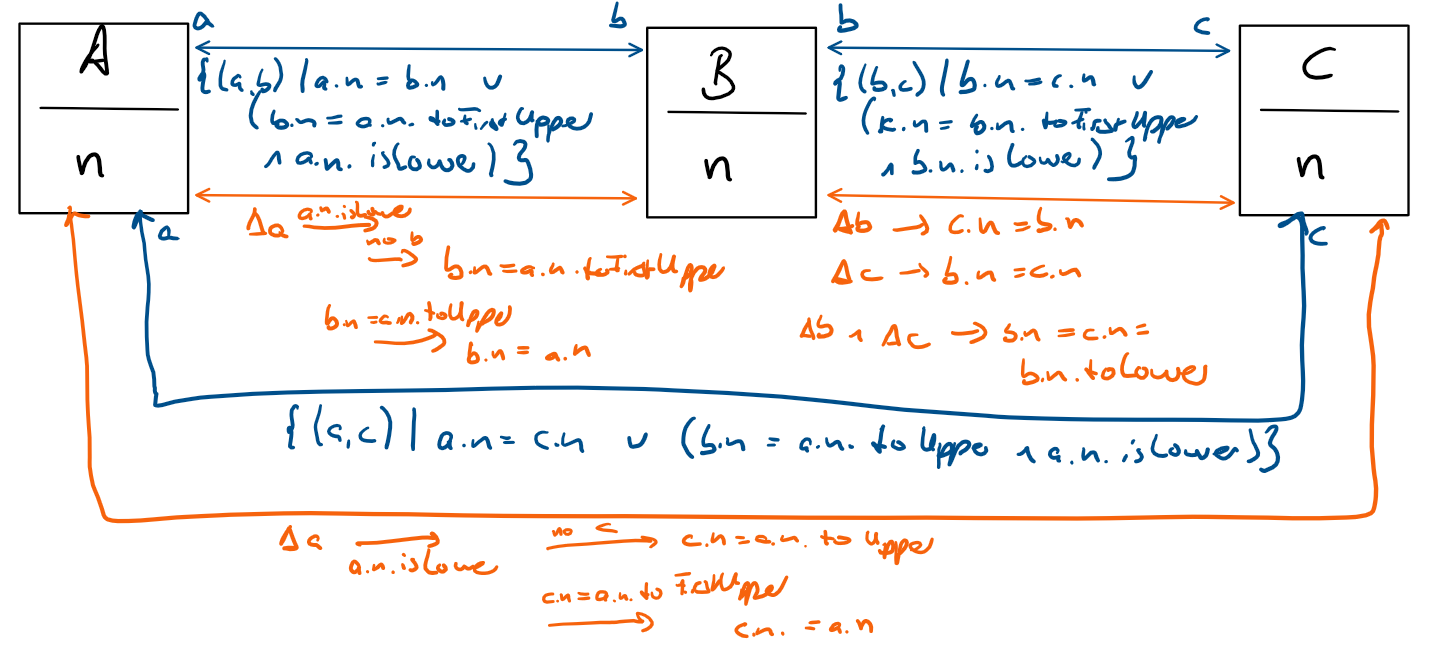
\includegraphics[width=\textwidth]{figures/correctness/orchestration/monotony_counterexample.png}
%     \caption{Counterexample for monotony}
%     \label{fig:formal:monotonycounterexample}
% \end{figure}

% One could now argue that there are binary relations in the example, which may never be fulfilled at all. We will later discuss how far relations that cannot be fulfilled should be restricted. However, in general, this is wanted behavior, because in general it may be necessary that transformations produce intermediate states that are not yet consistent with each other. Otherwise this would means that each transformation is always able to directly deliver a state that is consistent to all other relations, which is especially not possible, because other transformations may add further information to the models. More precisely, a relation may consider <a model consistent to all other models that contain any additional information not affected by the transformation. For example, a UML class model may be considered consistent to all Java models with any implementation of the specified methods, thus to an infinite number of models. Now saying that it should not be allowed that the transformation selects one with an empty implementation because that is not consistent to another relations induced by another transformation, such as the relationship to a component model, does not make any sense. Thus having those relation elements that may be considered locally consistent but will never occur in a globally consistent tuple of models does not make sense.
% In the example, we can see that such an inconsistent intermediate state is passed through and afterwards a consistent tuple of models is reached if not requiring monotony.
% In consequence, requiring monotony from transformations is a too strict requirement, because it is necessary to run through states that may be changed later on.

% \begin{theorem}
%     An application function for monotone transformations either returns a consistent model or produce a sequence of CPRs returning delta that return models of always growing size (i.e. it diverges).
% \end{theorem}


% \paragraph{Divergence cannot be avoided}

% There are rather equal network, one that terminates after a long time and one that never terminates. 
% Consider the example. The relations are defined in a way such that for any allocation for any of them a consistent tuple of models can be found. However, the transformations are not able to find it because they make "bad" choices from a set of choices that are conflicting. 
% This can be seen in the example that we have already given in \autoref{fig:correctness:no_execution_order}.

% Thus, systematically avoiding divergence is not possible. 



% \paragraph{Detecting Alternation / Divergence}

% In consequence, we propose to dynamically deal with alternation / divergence.
% To detect alternations, the execution can simply track if a state way already processed. Apart from spatial problems, this does always work.
% Finding divergence is not that easy, because it is generally not possible to define an upper bound for the number of executions of a single transformation.
% This is due to the reason that, again, this conflicts with the Halting problem.
% We can see this at the simple example in \autoref{fig:formal:noupperboundexample}.

% \begin{figure}
%     \centering
%     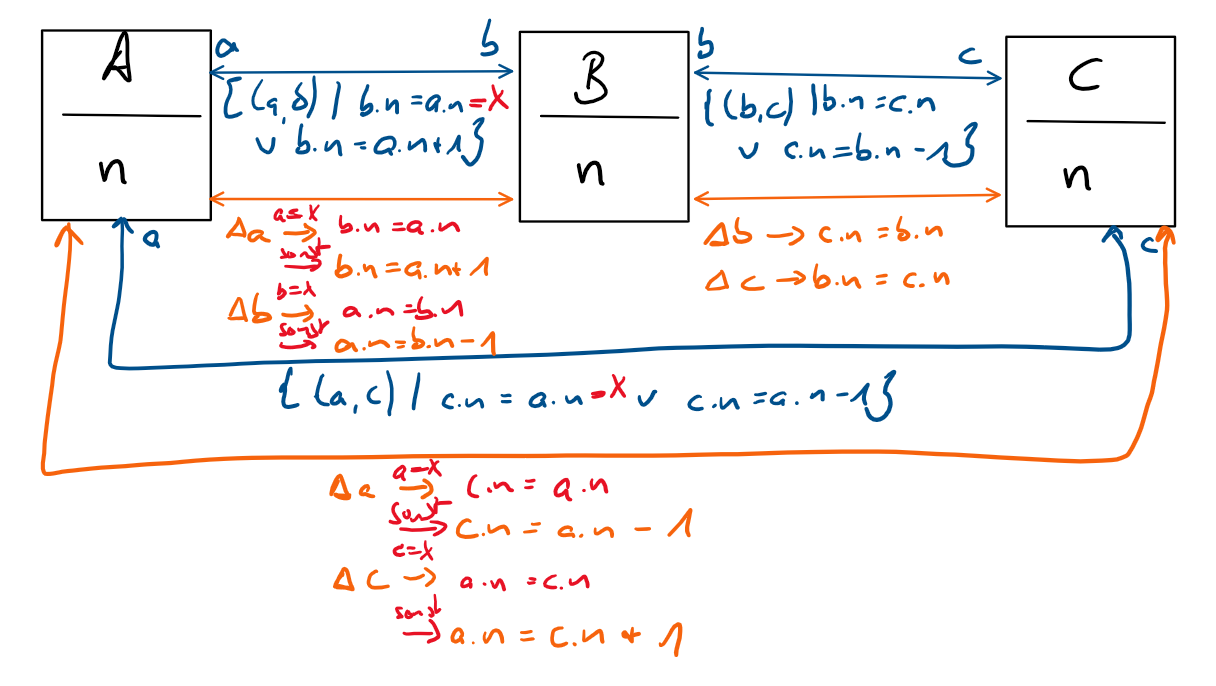
\includegraphics[width=\textwidth]{figures/correctness/orchestration/no_upper_bound_example.png}
%     \caption{Example for no upper bound}
%     \label{fig:formal:noupperboundexample}
% \end{figure}

% Depending on the value X, the transformations have to be executed X times to result in a consistent state. This value can be arbitrarily chosen, thus an arbitrary number of executions may be necessary to terminate in a consistent state.

% From an engineering perspective, this is still unwanted behavior. We claim that a transformation network that takes thousands of executions of the same transformation to find a consistent state works not as expected and if running into a failure would expose severe problems to find the reasons for that failures.
% Thus, we propose to simply abort the execution after some time to be sure not to run in an endless loop.

% Finally, this problem is comparable to ordinary programming, because there the same situations regarding alternation and divergence can occur that result in non-termination of a program.
% As we all know, it is impossible to systematically avoid that, but just possible to carefully develop the program and apply best practices to avoid such situations.

% In the following, we propose measures to reduce the number of cases in which problematic cases can occur.
% In a case study, we will see that using such measures already resolves most of the problems that can occur.
% Additionally, we propose an orchestration strategy that improves the possibility to find errors in case something goes wrong.

% \textbf{Central insight:} Alternation / Divergence cannot be avoided systematically (like in ordinary programming), if not restricting transformations in a way that may not be reasonable.

% \subsection{Reducing Conservativeness of the Application Function}

% Goal: Find a solution in as many cases as possible, abort in the others (conservatively). There are two approaches to achieve that: 
% 1. Reduce the number of cases in which there is no solution by adding assumptions to the relations and transformations (restrict input of app function)
% 2. Improve the ability to find a solution if it exists (improve capabilities of app function)
% Secondary goal: In cases, in which no solution is found, support the user in understanding why no solution was found.


% Regarding 1: Reduce problematic cases


% 1. reduce cases in which there is no such solution
% 1.1. On relation level: Only sets, so analysis possible.
% Ensure that relations are defined in a way such that they do not allow a locally correct set of CPRs that has no APP solution. If there is a pair of models (or elements of a fine-grained relation) in a relation, a CPR may return it. But if there is no consistent tuple of models containing these two, it does not make any sense to consider these elements (even worse, if we have monotony, adding these elements makes the network unsolvable). For that reason, we need compatibility. Avoids both alternation and divergence
% 1.2. On transformation level: Hard to perform analyses
% Require monotony to avoid alternation
% Give some example why divergence cannot easily be avoided, thus terminate at some point
% 2. find the solution in as many cases as possible -> reasonable orchestration strategy
% Focus on engineering solution 


% Thus, there arise two questions:
% - Although theoretically easy, how to practically define a CPR that is synchronizing?
% - How to define an APP function and which requirements does that impose?




% \section{Optimality rather than Correctness}

% \mnote{Achieving a correct application function}
% The definition of the application function basically ensures that the function either returns $\bot$ or executes the \modellevelconsistencypreservationrules given by the orchestration function to retrieve a changes tuple of models.
% It is considered \emph{correct} if it ensures that its result is either $\bot$ or a consistent model tuple by executing the \modellevelconsistencypreservationrules given by the orchestration function.
% % A correct application function thus has to ensure that its result is either $\bot$ or a consistent model tuple by executing the \modellevelconsistencypreservationrules given by the orchestration function.
% In consequence, the application function can be realized by simply executing the result of the orchestration function and check whether the resulting model tuple is consistent or not and return an appropriate result.
% Such a realization is generic and does not depend on the actual consistency preservation rules and orchestration function but represents a generic behavior.
% Additionally, this gives an implementation of that function the ability to present a faulty result to the user, which eases finding out why no consistent state was reached.

% \mnote{Correctness is not crucial}
% Finally, correctness is not crucial, because correctness can easily be achieved by performing any execution of transformations and just ensuring that we terminate at some point in time and then decide whether the resulting models are consistent or not and appropriately deliver the result.

% \mnote{How to define an orchestration function that is as optimal as possible?}
% The remaining difficulty is how to define an orchestration function that fulfills the definition, i.e., to find a finite sequence of transformations, and also one that improves optimality, as an \emph{optimal} function can never be given.
% Although the definition of the orchestration function proposes a closed description of that function, in practice such a function will not have a closed form but will be realized as an algorithm that dynamically decides which transformation to execute next.
% Therefore the arising problem is that the length of the sequence to execute is not known a priori. Therefore, we need some abortion criterion. When a consistent result is found, this criterion is easy. But since we do not know whether a sequence exist, we need an abortion criterion that is reasonable and does not cut off the process although a consistent solution could be found, thus reducing optimality.
% A simple realization for that algorithm to deliver a finite sequence of transformations would be to define a fixed termination criterion, such as a specific number of transformation executions. However, there is no upper bound for the number of executed transformations necessary to achieve consistency. Still, a fixed number (even 0) could be defined for the number of executed transformations to fulfill the definition. Hence, optimality would be 0 then as a consistent result is never reached. We therefore discuss in the following how to define an appropriate orchestration function and how to optimize it.

% \mnote{Achieving a correct application function}
% The definition of the application function basically ensures that the function either returns $\bot$ or executes the \modellevelconsistencypreservationrules given by the orchestration function to retrieve a changes tuple of models.
% It is considered \emph{correct} if it ensures that its result is either $\bot$ or a consistent model tuple by executing the \modellevelconsistencypreservationrules given by the orchestration function.
% % A correct application function thus has to ensure that its result is either $\bot$ or a consistent model tuple by executing the \modellevelconsistencypreservationrules given by the orchestration function.
% In consequence, the application function can be realized by simply executing the result of the orchestration function and check whether the resulting model tuple is consistent or not and return an appropriate result.
% Such a realization is generic and does not depend on the actual consistency preservation rules and orchestration function but represents a generic behavior.
% Additionally, this gives an implementation of that function the ability to present a faulty result to the user, which eases finding out why no consistent state was reached.

% \mnote{Correctness is not crucial}
% Finally, correctness is not crucial, because correctness can easily be achieved by performing any execution of transformations and just ensuring that we terminate at some point in time and then decide whether the resulting models are consistent or not and appropriately deliver the result.

% \mnote{How to define an orchestration function that is as optimal as possible?}
% The remaining difficulty is how to define an orchestration function that fulfills the definition, i.e., to find a finite sequence of transformations, and also one that improves optimality, as an \emph{optimal} function can never be given.
% Although the definition of the orchestration function proposes a closed description of that function, in practice such a function will not have a closed form but will be realized as an algorithm that dynamically decides which transformation to execute next.
% Therefore the arising problem is that the length of the sequence to execute is not known a priori. Therefore, we need some abortion criterion. When a consistent result is found, this criterion is easy. But since we do not know whether a sequence exist, we need an abortion criterion that is reasonable and does not cut off the process although a consistent solution could be found, thus reducing optimality.
% A simple realization for that algorithm to deliver a finite sequence of transformations would be to define a fixed termination criterion, such as a specific number of transformation executions. However, there is no upper bound for the number of executed transformations necessary to achieve consistency. Still, a fixed number (even 0) could be defined for the number of executed transformations to fulfill the definition. Hence, optimality would be 0 then as a consistent result is never reached. We therefore discuss in the following how to define an appropriate orchestration function and how to optimize it.

% \textbf{Overall Goal:} Find correct orchestration function that improves optimality.

% There are two ways to improve optimality of the orchestration function:
% \begin{enumerate}
%     \item Optimize the orchestration function, i.e., find a good order (probably this is not possible), at least find an order that helps the developer to find problems
%     \item Optimize the input, i.e., define requirements to the transformations and their relations representing the input to optimize optimality
% \end{enumerate}
% \todo{We need an example for that}

% Both goes hand in hand, because restrictions to the input can never lead to an orchestration function that always terminates without leading to unsupported relevant cases.

% This conform to two approaches:
% \begin{enumerate}
%     \item Dynamic decision about selected transformation and abortion criteria
%     \item Constructive restrictions that ensure that appropriate order is (easily) found
% \end{enumerate}

% \todo{Application function can be generically defined, orchestration maybe not? We actually want to ensure that both are generic and none of them has to be defined for a specific project.}

